% Compile with: latexmk -pdf main.tex
% All text, mathematics, tables, and plots are editable LaTeX source.
\documentclass[t,aspectratio=169,11pt]{beamer}
% Beamer style rebuilt from the supplied lecture3.pdf reference.
% Standard TeX Live / Overleaf packages only. No system font paths.
\usepackage[T1]{fontenc}
\usepackage[utf8]{inputenc}
\usepackage{lmodern}
\usefonttheme[onlymath]{serif}
\usepackage{amsmath,amssymb,mathtools,bm}
\usepackage{booktabs,tabularx,array}
\usepackage{graphicx}
\usepackage{tikz,pgfplots}
\usepackage[most]{tcolorbox}
\usepackage{pgfpages}
\pgfplotsset{compat=1.18}
\usetikzlibrary{calc,arrows.meta,positioning}

\definecolor{titlered}{HTML}{D62B09}
\definecolor{bulletgreen}{HTML}{A8C99F}
\definecolor{definitionblue}{HTML}{E9F0F9}
\definecolor{takeawaypeach}{HTML}{FBECE6}
\definecolor{blueplot}{HTML}{4E79A7}
\definecolor{redplot}{HTML}{D95F59}
\definecolor{lightplot}{HTML}{8FB8DA}
\definecolor{inkplot}{HTML}{111111}
\setbeamercolor{normal text}{fg=black,bg=white}
\setbeamercolor{frametitle}{fg=titlered,bg=white}
\setbeamercolor{structure}{fg=titlered}
\setbeamercolor{itemize item}{fg=bulletgreen}
\setbeamercolor{itemize subitem}{fg=bulletgreen}
\setbeamercolor{footline}{fg=black,bg=white}
\setbeamercolor{block title}{fg=black,bg=definitionblue}
\setbeamercolor{block body}{fg=black,bg=definitionblue}
\setbeamersize{text margin left=0.75cm,text margin right=0.75cm}
\setbeamerfont{frametitle}{size=\fontsize{22}{25},series=\bfseries}
\setbeamerfont{footline}{size=\fontsize{5.5}{7}\selectfont}
\setbeamertemplate{navigation symbols}{}
\setbeamertemplate{itemize item}{\raise0.1ex\hbox{\small$\bullet$}}
\setbeamertemplate{itemize subitem}{\raise0.1ex\hbox{\scriptsize$\bullet$}}
\setbeamertemplate{frametitle}{%
  \vskip0.08cm
  \begin{beamercolorbox}[wd=\textwidth,center,sep=0pt]{frametitle}
    \usebeamerfont{frametitle}\strut\insertframetitle\strut\par
  \end{beamercolorbox}
  \vskip0.25cm
}
\setbeamertemplate{footline}{%
  \begin{beamercolorbox}[wd=\paperwidth,ht=0.25cm,dp=0.10cm,center]{footline}
    \usebeamerfont{footline}\insertframenumber
  \end{beamercolorbox}
}
\setlength{\parskip}{3pt}
\setlength{\abovedisplayskip}{6pt}
\setlength{\belowdisplayskip}{6pt}
\setlength{\abovedisplayshortskip}{4pt}
\setlength{\belowdisplayshortskip}{4pt}

\newcommand{\lead}[1]{{\small #1\par}\vspace{0.12cm}}
\newtcolorbox{definitionbox}{enhanced,colback=definitionblue,
  colframe=definitionblue,boxrule=0pt,arc=3pt,
  fontupper=\small,
  before upper={\setlength{\abovedisplayskip}{4pt}\setlength{\belowdisplayskip}{4pt}\setlength{\jot}{2pt}},
  left=6pt,right=6pt,top=4pt,bottom=4pt,
  before skip=4pt,after skip=5pt}
\newtcolorbox{takeaway}{enhanced,colback=takeawaypeach,
  colframe=takeawaypeach,boxrule=0pt,arc=3pt,
  fontupper=\small,left=6pt,right=6pt,top=4pt,bottom=4pt,
  before skip=6pt,after skip=0pt}
\newcommand{\demolink}[1]{\href{https://regression-lab-graduate-2026.whu38f.chatgpt.site/\##1}{\textcolor{titlered}{\textbf{Open web demo: #1}}}}
\newcommand{\R}{\mathbb{R}}
\newcommand{\E}{\mathbb{E}}
\DeclareMathOperator{\Var}{Var}
\DeclareMathOperator{\Cov}{Cov}
\DeclareMathOperator{\diag}{diag}
\DeclareMathOperator{\Col}{Col}
\DeclareMathOperator{\rank}{rank}
\DeclareMathOperator*{\argmin}{arg\,min}
\newcolumntype{Y}{>{\raggedright\arraybackslash}X}
\setbeameroption{hide notes}


\newcommand{\olsstar}{\theta^{\star}}
\newcommand{\olshat}{\widehat\theta}
\newcommand{\olserr}{\widehat\theta-\theta^{\star}}
\newcommand{\olstr}{\operatorname{tr}}
\newcommand{\olsfigpath}{figures/}
\newcommand{\olsfig}[1]{\input{\olsfigpath#1.tex}}
\newcommand{\olsprompt}[1]{\textcolor{titlered}{\textbf{#1}}}


\title{Linear Regression}
\author{Zihan Zhang}
\institute{COMP 5212: Machine Learning}
\date{}
\hypersetup{
  pdftitle={Linear Regression},
  pdfauthor={Zihan Zhang},
  pdfsubject={Graduate Machine Learning: COMP 5212},
  pdfkeywords={linear regression, least squares, conditioning, ridge, lasso, polynomial features, kernels}
}
\newcommand{\SectionSlide}[2]{%
	\begin{frame}
		\centering
		\vfill
		{\color{slideorange}\fontsize{29}{34}\selectfont\bfseries #1\par}
		\vspace{0.38cm}
		{\color{midgray}\fontsize{16}{21}\selectfont #2\par}
		\vfill
	\end{frame}
}

\definecolor{slideorange}{HTML}{D62B09}
\definecolor{midgray}{HTML}{666666}
% Uncomment to include each slide with its speaker notes on a second screen.
% \setbeameroption{show notes on second screen=right}

\begin{document}
\begin{frame}
  \vspace{0.05cm}
  \hspace{-0.38cm}
\includegraphics[width=5.65cm]{assets/hkust-logo.png}
  \vspace{-0.15cm}
  \begin{center}
    {\fontsize{29}{35}\selectfont COMP 5212\par}
    \vspace{0.30cm}
    {\fontsize{32}{38}\selectfont Machine Learning\par}
    \vspace{0.35cm}
    {\fontsize{17}{21}\selectfont Instructor: Zihan Zhang\par}
    \vspace{0.25cm}
    {\fontsize{14}{18}\selectfont Lecture 4: Linear Regression\par}
    \vspace{0.12cm}
   
  \end{center}
\end{frame}

\begin{frame}[t]{Learning Goals}
	\vspace{0.03cm}
	{\fontsize{13.2}{16.2}\selectfont
		By the end of this lecture, you should be able to:
		\begin{itemize}
			\setlength{\itemsep}{0.18cm}
			\item formulate linear regression and justify the squared-error loss;
			\item derive and apply the ordinary least squares (OLS) solution;
			\item explain and compare Ridge and Lasso regularization;
			\item use polynomial features and kernels to model nonlinear relationships;
			\item interpret an OLS generalization bound and explain its assumptions.
		\end{itemize}
	}
\end{frame}

% English linear regression lecture. Exactly five sections.
% Cover in main.tex; detailed explanations remain in speaker notes.

% Slide 2 | roadmap

% Slide 3 | section-1
\SectionSlide{Motivation Example}{}

% Slide 4 | motivation-1
\begin{frame}{Tomorrow's electricity use?}
\lead{A factory plans to produce $5.5$ tonnes tomorrow.}
\begin{columns}[c,onlytextwidth]
\begin{column}{.52\textwidth}\centering
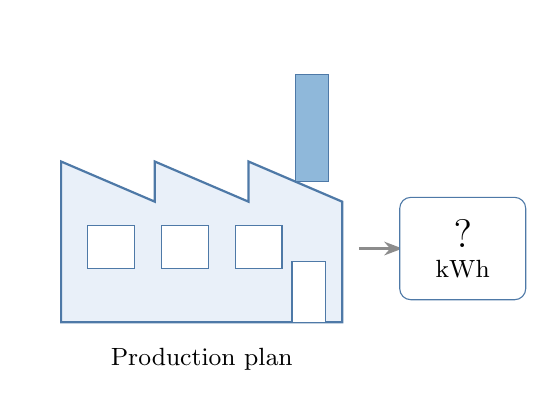
\begin{tikzpicture}[x=.85cm,y=.85cm]
\useasboundingbox (-.5,-.9) rectangle (7,4.4);
\path[fill=definitionblue,draw=blueplot,thick] (0,0)--(0,2.4)--(1.4,1.8)--(1.4,2.4)--(2.8,1.8)--(2.8,2.4)--(4.2,1.8)--(4.2,0)--cycle;
\path[fill=lightplot,draw=blueplot] (3.5,2.1) rectangle (4,3.7);
\foreach \x in {.4,1.5,2.6}{\path[fill=white,draw=blueplot] (\x,.8) rectangle +(0.7,.65);}
\path[fill=white,draw=blueplot] (3.45,0) rectangle +(0.5,.9);
\draw[-{Stealth},thick,black!45] (4.45,1.1)--(5.1,1.1);
\node[draw=blueplot,rounded corners,fill=white,minimum width=1.6cm,minimum height=1.3cm,align=center] at (6,1.1) {\Large ?\\[-1pt]\small kWh};
\node[anchor=north,align=center,font=\small] at (2.1,-.25) {Production plan};
\end{tikzpicture}
\end{column}
\begin{column}{.43\textwidth}
\begin{overlayarea}{\linewidth}{3.4cm}
\only<1>{\vspace{.65cm}\Large What would you measure?}
\only<2>{\small\textbf{Past daily records}\par\medskip
Production + electricity\par\medskip
Weather + shifts\par\bigskip
\textbf{Tomorrow's target}\par\medskip
Electricity use}
\only<3>{\large Inputs $x$\par\medskip
$\downarrow$\par\medskip
Prediction $\widehat y$\par\medskip
\small Budgeting\quad Energy monitoring}
\end{overlayarea}
\end{column}
\end{columns}
\end{frame}

% Slide 5 | motivation-2
\begin{frame}{Tomorrow's electricity use?}
\lead{Tomorrow: $5.5$ tonnes. Your forecast?}
\begin{columns}[c,onlytextwidth]
\begin{column}{.59\textwidth}% Constructed daily production/electricity observations; stages hide both answers.
\begin{tikzpicture}
\begin{axis}[width=\linewidth,height=4.65cm,font=\scriptsize,
 xmin=3.8,xmax=6.2,ymin=150,ymax=250,xtick={4,4.5,5,5.5,6},ytick={160,180,200,220,240},
 xlabel={Production (tonnes/day)},ylabel={Electricity (kWh/day)},
 grid=major,grid style={black!8},axis line style={black!40},tick style={black!40},
 scaled ticks=false,clip=true]
\addplot[only marks,mark=*,mark size=2pt,black!75] coordinates {
 (4.0,164.00) (4.2,178.92) (4.4,174.08) (4.6,189.48) (4.8,191.12)
 (5.0,206.00) (5.2,204.12) (5.4,218.48) (5.6,217.08) (5.8,231.92) (6.0,238.00)};
\only<2->{\addplot[lightplot,densely dashed,very thick,domain=3.8:6.2]{201.2};}
\only<3->{
 \addplot[blueplot,very thick,domain=3.8:6.2]{23.4727272727+35.5454545455*x};
 \draw[redplot,densely dashed] (axis cs:5.5,150)--(axis cs:5.5,218.9727272727);
 \addplot[only marks,mark=*,mark size=3pt,redplot] coordinates {(5.5,218.9727272727)};
}
\end{axis}
\end{tikzpicture}
\end{column}
\begin{column}{.37\textwidth}
\begin{overlayarea}{\linewidth}{3.6cm}
\only<1>{\vspace{.7cm}\Large One number?\par\medskip\small Explain your choice.}
\only<2>{\textcolor{lightplot}{\textbf{Ignore production}}\par\medskip
\Large $\overline y=201.2$\par\medskip\small kWh/day\par\bigskip
Where does this miss?}
\only<3>{\textcolor{blueplot}{\textbf{Use production}}\par\medskip
\large $\widehat y=b+wx$\par\medskip
\Large $\widehat y(5.5)\approx219$\par\medskip\small kWh/day}
\end{overlayarea}
\end{column}
\end{columns}
\end{frame}

% Slide 6 | motivation-3
\begin{frame}{But the world is nonlinear}
\lead{Would one straight line work everywhere?}
\begin{columns}[c,onlytextwidth]
\begin{column}{.59\textwidth}\begin{tikzpicture}
\begin{axis}[width=\linewidth,height=4.65cm,font=\scriptsize,
 xmin=0,xmax=10,ymin=0,ymax=470,xtick={0,2,4,6,8,10},ytick={0,100,200,300,400},
 xlabel={Production (tonnes/day)},ylabel={Mean electricity (kWh/day)},
 grid=major,grid style={black!8},axis line style={black!40},tick style={black!40},scaled ticks=false]
\only<2->{\path[fill=bulletgreen,opacity=.35] (axis cs:4,0) rectangle (axis cs:6,470);}
\addplot[blueplot,very thick,domain=0:10,samples=80]{100+5*x+3*x*x};
\only<3->{
 \addplot[redplot,thick,dashed,domain=0:10]{25+35*x};
 \addplot[black,only marks,mark=*,mark size=2pt] coordinates {(5,200)};
}
\end{axis}
\end{tikzpicture}
\end{column}
\begin{column}{.37\textwidth}
\begin{overlayarea}{\linewidth}{3.7cm}
\only<1>{\vspace{.6cm}\large Suppose the true mean looks like this.\par\bigskip
Reject a linear model?}
\only<2>{\vspace{.4cm}\large Where do we operate?\par\bigskip
\small Observed range:\par\medskip
\large $4\leq x\leq6$}
\only<3>{\vspace{.3cm}\textcolor{blueplot}{\textbf{Curved mean}}\par\medskip
\textcolor{redplot}{\textbf{Local tangent}}\par\bigskip
\large Close here.\par\medskip
Different elsewhere.}
\end{overlayarea}
\end{column}\end{columns}
\end{frame}

% Slide 7 | motivation-4
\begin{frame}{Zoom in. What changes?}
\lead{Same curve. Same tangent. Smaller neighborhoods.}
\vspace{.15cm}
% All panels plot the same mean m(x)=100+5x+3x^2 and tangent at x0=5.
\begingroup
\pgfplotsset{motivationzoom/.style={width=\linewidth,height=3.45cm,font=\scriptsize,
 xlabel={$x$ (tonnes/day)},ylabel={$m(x)$ (kWh/day)},
 grid=major,grid style={black!8},axis line style={black!40},tick style={black!40},
 scaled ticks=false,tick label style={/pgf/number format/fixed},samples=65}}
\begin{columns}[T,onlytextwidth]
\begin{column}{.315\textwidth}\centering
\small $|x-5|\leq 5$\par
\begin{tikzpicture}\begin{axis}[motivationzoom,xmin=0,xmax=10,ymin=0,ymax=470,xtick={0,5,10},ytick={0,200,400}]
\addplot[blueplot,very thick,domain=0:10]{100+5*x+3*x*x};
\addplot[redplot,thick,dashed,domain=0:10]{25+35*x};
\end{axis}\end{tikzpicture}\par
\small Max. gap: $75$ kWh
\end{column}
\begin{column}{.315\textwidth}\centering\uncover<2->{
\small $|x-5|\leq 1$\par
\begin{tikzpicture}\begin{axis}[motivationzoom,xmin=4,xmax=6,ymin=158,ymax=245,xtick={4,5,6},ytick={160,200,240}]
\addplot[blueplot,very thick,domain=4:6]{100+5*x+3*x*x};
\addplot[redplot,thick,dashed,domain=4:6]{25+35*x};
\end{axis}\end{tikzpicture}\par
\small Max. gap: $3$ kWh}
\end{column}
\begin{column}{.315\textwidth}\centering\uncover<3->{
\small $|x-5|\leq 0.2$\par
\begin{tikzpicture}\begin{axis}[motivationzoom,xmin=4.8,xmax=5.2,ymin=191,ymax=209,xtick={4.8,5,5.2},ytick={192,200,208}]
\addplot[blueplot,very thick,domain=4.8:5.2]{100+5*x+3*x*x};
\addplot[redplot,thick,dashed,domain=4.8:5.2]{25+35*x};
\end{axis}\end{tikzpicture}\par
\small Max. gap: $0.12$ kWh}
\end{column}
\end{columns}
\endgroup

\vspace{.15cm}
\centering{\scriptsize\textcolor{blueplot}{Solid: mean}\qquad\textcolor{redplot}{Dashed: tangent}\qquad Each panel rescales its axes.}
\vfill
\uncover<3->{\begin{takeaway}Useful range depends on curvature, noise, and required accuracy.\end{takeaway}}
\note{Suggested time: 4 minutes. Build 1: show only the wide-range panel. Ask what students expect if we zoom around x=5, and pause for 10 seconds. Build 2: reveal the middle panel, whose range matches the previous observations. Pause again before asking how large the approximation error now is relative to the several-kWh deviations in the scatterplot. Build 3: reveal the narrow panel. All panels use the same m(x)=100+5x+3x squared and tangent L(x)=25+35x. The exact difference is m(x)-L(x)=3(x-5) squared, so the maximum gaps are 75, 3, and 0.12 kWh on radii 5, 1, and 0.2. Both horizontal and vertical axes are rescaled, and the numerical gaps prevent a misleading purely visual claim. Smaller neighborhoods improve this smooth approximation but may contain fewer samples for estimation. Noise size here is illustrative; do not imply that these finite data determine the population noise variance. The derivative predicts first-order change, not exact equality on a finite interval.}
\end{frame}

% Slide 8 | motivation-5
\begin{frame}{Why linear models appear everywhere}
\lead{What is the first change near an operating point?}
\begin{overlayarea}{\textwidth}{4.5cm}
\only<1>{\vspace{1cm}\centering
\Large $x_0\ \longrightarrow\ x_0+h$\par\bigskip
\large What happens to $m(x)$?}
\only<2>{\vspace{.55cm}
\begin{definitionbox}\[
\underbrace{m(x_0+h)}_{\text{nearby mean}}
\ \approx\ \underbrace{m(x_0)}_{\text{level}}
+\underbrace{m'(x_0)}_{\text{slope}}h.
\]\end{definitionbox}
\vspace{.45cm}\centering\large Level $+$ sensitivity $\times$ change}
\only<3>{\vspace{.4cm}
\begin{definitionbox}\[
\begin{aligned}
m(x_0+h)&\approx m(x_0)+\nabla m(x_0)^{\mathsf T}h,\\[4pt]
&=b+w^{\mathsf T}x,\qquad x=x_0+h.
\end{aligned}
\]\end{definitionbox}
\vspace{.25cm}\centering\small $w=\nabla m(x_0),\qquad b=m(x_0)-w^{\mathsf T}x_0$}
\end{overlayarea}
\end{frame}


\begin{frame}{Why linear models appear everywhere}
	Linear relationships arise naturally in many settings.
	
	\medskip
	\begin{columns}[T,onlytextwidth]
		\begin{column}{0.47\textwidth}
			\centering
			\textbf{Physical laws}
			
			\medskip
			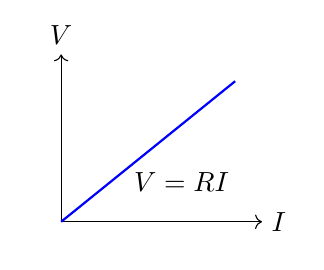
\begin{tikzpicture}[scale=0.85]
				\path[use as bounding box]
				(-0.5,-0.3) rectangle (3.5,2.9);
				\draw[->] (0,0) -- (3,0) node[right] {$I$};
				\draw[->] (0,0) -- (0,2.5) node[above] {$V$};
				\draw[blue,thick] (0,0) -- (2.6,2.1);
				\node at (1.8,0.6) {$V=RI$};
			\end{tikzpicture}
			
			\par\smallskip
			{\small
				Ohm's law: voltage is proportional to current
				for a fixed resistance.\par
			}
		\end{column}
		\hspace{0.06\textwidth}%
		\begin{column}{0.47\textwidth}
			\centering
			\textbf{Economic models}
			
			\medskip
			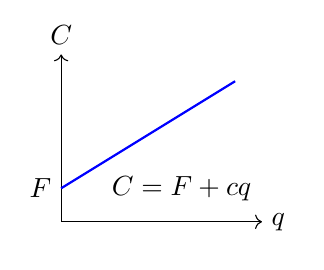
\begin{tikzpicture}[scale=0.85]
				\path[use as bounding box]
				(-0.5,-0.3) rectangle (3.5,2.9);
				\draw[->] (0,0) -- (3,0) node[right] {$q$};
				\draw[->] (0,0) -- (0,2.5) node[above] {$C$};
				\draw[blue,thick] (0,0.5) -- (2.6,2.1);
				\node[left] at (0,0.5) {$F$};
				\node at (1.8,0.5) {$C=F+cq$};
			\end{tikzpicture}
			
			\par\smallskip
			{\small
				Total cost is linear in output when
				marginal cost is constant.\par
			}
		\end{column}
	\end{columns}
\end{frame}

% Slide 9 | motivation-6
\begin{frame}{How much complexity do we need?}
\lead{Unknown curvature. Limited observations. A new prediction task.}
\begin{overlayarea}{\textwidth}{4.5cm}
\only<1>{\vspace{.85cm}\centering
\Large Straight line?\qquad Polynomial?\qquad Neural network?\par\bigskip
\large What would you try first?}
\only<2>{\vspace{.65cm}\centering
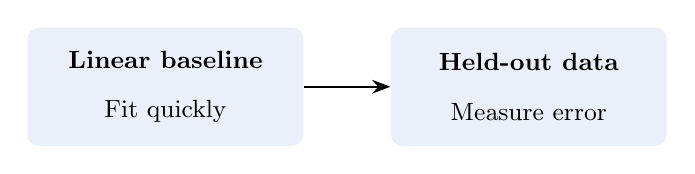
\begin{tikzpicture}[every node/.style={align=center,font=\small}]
\node[fill=definitionblue,rounded corners,minimum width=3.5cm,minimum height=1.5cm] (a) {\textbf{Linear baseline}\\[7pt]Fit quickly};
\node[fill=definitionblue,rounded corners,minimum width=3.5cm,minimum height=1.5cm,right=1.1cm of a] (b) {\textbf{Held-out data}\\[7pt]Measure error};
\draw[-{Stealth},thick] (a)--(b);
\end{tikzpicture}\par\bigskip
\large A first benchmark, before adding complexity.}
\only<3>{\vspace{.4cm}\centering
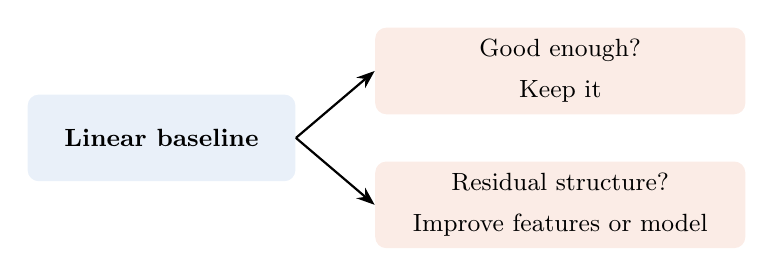
\begin{tikzpicture}[every node/.style={align=center,font=\small}]
\node[fill=definitionblue,rounded corners,minimum width=3.4cm,minimum height=1.1cm] (a) {\textbf{Linear baseline}};
\node[fill=takeawaypeach,rounded corners,minimum width=4.7cm,minimum height=1.1cm,right=1cm of a,yshift=.85cm] (b) {Good enough?\\[4pt]Keep it};
\node[fill=takeawaypeach,rounded corners,minimum width=4.7cm,minimum height=1.1cm,right=1cm of a,yshift=-.85cm] (c) {Residual structure?\\[4pt]Improve features or model};
\draw[-{Stealth},thick] (a.east)--(b.west);
\draw[-{Stealth},thick] (a.east)--(c.west);
\end{tikzpicture}}
\end{overlayarea}
\vfill
\uncover<2->{\begin{takeaway}An inexpensive starting point; adequacy is an empirical question.\end{takeaway}}
\note{Suggested time: 3 minutes. Build 1: invite a vote and pause for 15 seconds. Interpret unknown scale broadly: we may not yet know the sample size needed, the relevant input range, the curvature, or how accurate the application requires predictions to be. Build 2: suggest a simple linear baseline because it is comparatively easy to fit, inspect, and compare. This is a modeling heuristic, not a theorem that linear regression is universally optimal or literally always appropriate. Strong prior knowledge, structural constraints, or the target type may point elsewhere immediately. Build 3: reveal the next decision only after asking what evidence would justify more complexity. Evaluate on a validation split matching intended use, inspect residual patterns, and consider interactions, transformed features, regularization, or a different model. A repeated pattern is a diagnostic lead, not proof of a particular mechanism. Reserve a final test set for the end of model selection. Linear models remain useful benchmarks even when a more flexible model eventually wins.}
\end{frame}

% Slide 10 | section-2

\SectionSlide{Formulation and closed-form derivation}{}


% Slide 11 | lsq-10
\begin{frame}{Linear in the parameters}
\begin{definitionbox}
\[
 f_{\theta}(x)=b+w^{\mathsf T}x \qquad \theta= [b,w]^{\top}
\]
\end{definitionbox}
\small
\begin{itemize}\setlength{\itemsep}{8pt}
\item Weights enter linearly in input.
\item The intercept $b$ is the prediction when every feature is zero.
\end{itemize}
\end{frame}

% Slide 12 | lsq-11
\begin{frame}{What counts as a good fit?}
\lead{Squared loss gives larger errors more weight}
\begin{columns}[T,onlytextwidth]
\begin{column}{0.55\textwidth}% Generated from work/deck/chart-data-en.mjs; numeric data preserved.
% Input in a column; rocpr is intended for full frame width.
\begingroup
\definecolor{blueplot}{HTML}{4E79A7}
\definecolor{redplot}{HTML}{D95F59}
\definecolor{inkplot}{HTML}{111111}
\definecolor{lightplot}{HTML}{8FB8DA}
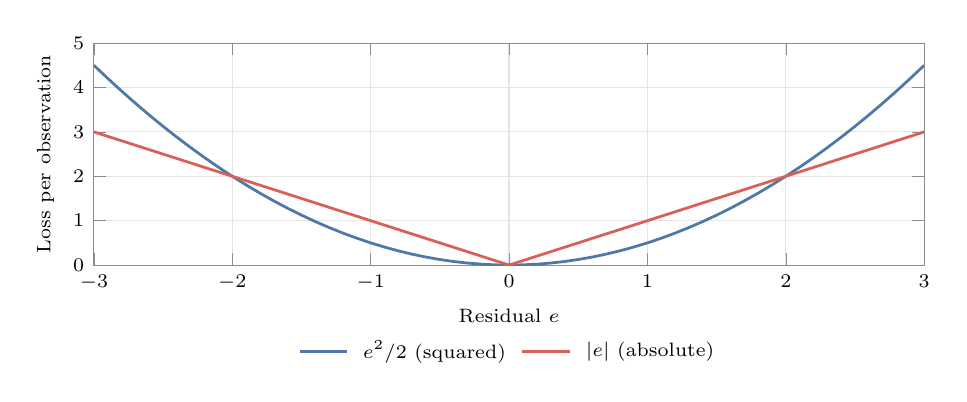
\begin{tikzpicture}
\begin{axis}[
width=\linewidth,
height=4.4cm,
font=\scriptsize,
tick label style={font=\scriptsize},
label style={font=\scriptsize},
axis line style={black!45},
tick style={black!45},
grid=major,
grid style={black!10},
xmin=-3,
xmax=3,
ymin=0,
ymax=5,
xlabel={Residual $e$},
ylabel={Loss per observation},
scaled ticks=false,
tick label style={/pgf/number format/fixed},
clip=true,
unbounded coords=jump,
legend style={font=\scriptsize,draw=none,fill=none,at={(0.5,-0.29)},anchor=north,legend cell align=left,column sep=0.12cm,row sep=0.03cm},
legend columns=-1,
xtick={-3,-2,-1,0,1,2,3},
ytick={0,1,2,3,4,5}
]
\addplot+[no marks,draw=blueplot,line width=1pt] coordinates {(-3,4.5) (-2.9,4.205) (-2.8,3.92) (-2.7,3.645) (-2.6,3.38) (-2.5,3.125) (-2.4,2.88) (-2.3,2.645) (-2.2,2.42) (-2.1,2.205) (-2,2) (-1.9,1.805) (-1.8,1.62) (-1.7,1.445) (-1.6,1.28) (-1.5,1.125) (-1.4,0.98) (-1.3,0.845) (-1.2,0.72) (-1.1,0.605) (-1,0.5) (-0.9,0.405) (-0.8,0.32) (-0.7,0.245) (-0.6,0.18) (-0.5,0.125) (-0.4,0.08) (-0.3,0.045) (-0.2,0.02) (-0.1,0.005) (0,0) (0.1,0.005) (0.2,0.02) (0.3,0.045) (0.4,0.08) (0.5,0.125) (0.6,0.18) (0.7,0.245) (0.8,0.32) (0.9,0.405) (1,0.5) (1.1,0.605) (1.2,0.72) (1.3,0.845) (1.4,0.98) (1.5,1.125) (1.6,1.28) (1.7,1.445) (1.8,1.62) (1.9,1.805) (2,2) (2.1,2.205) (2.2,2.42) (2.3,2.645) (2.4,2.88) (2.5,3.125) (2.6,3.38) (2.7,3.645) (2.8,3.92) (2.9,4.205) (3,4.5)};
\addlegendentry{$e^2/2$ (squared)}
\addplot+[no marks,draw=redplot,line width=1pt] coordinates {(-3,3) (-2.9,2.9) (-2.8,2.8) (-2.7,2.7) (-2.6,2.6) (-2.5,2.5) (-2.4,2.4) (-2.3,2.3) (-2.2,2.2) (-2.1,2.1) (-2,2) (-1.9,1.9) (-1.8,1.8) (-1.7,1.7) (-1.6,1.6) (-1.5,1.5) (-1.4,1.4) (-1.3,1.3) (-1.2,1.2) (-1.1,1.1) (-1,1) (-0.9,0.9) (-0.8,0.8) (-0.7,0.7) (-0.6,0.6) (-0.5,0.5) (-0.4,0.4) (-0.3,0.3) (-0.2,0.2) (-0.1,0.1) (0,0) (0.1,0.1) (0.2,0.2) (0.3,0.3) (0.4,0.4) (0.5,0.5) (0.6,0.6) (0.7,0.7) (0.8,0.8) (0.9,0.9) (1,1) (1.1,1.1) (1.2,1.2) (1.3,1.3) (1.4,1.4) (1.5,1.5) (1.6,1.6) (1.7,1.7) (1.8,1.8) (1.9,1.9) (2,2) (2.1,2.1) (2.2,2.2) (2.3,2.3) (2.4,2.4) (2.5,2.5) (2.6,2.6) (2.7,2.7) (2.8,2.8) (2.9,2.9) (3,3)};
\addlegendentry{$|e|$ (absolute)}
\end{axis}
\end{tikzpicture}
\endgroup
\end{column}
\begin{column}{0.42\textwidth}\small
Residual: $e_i=y_i-f_{\theta}(x_i)$.
\[
 J(\theta)=\frac{1}{2n}\sum_{i=1}^n e_i^2.
\]
\begin{itemize}\setlength{\itemsep}{10pt}
\item $1/2$ simplifies derivatives.
\item $1/n$ normalizes sample size.
\end{itemize}
\end{column}\end{columns}
\end{frame}






% Slide 17 | lsq-20
\begin{frame}{Build the design matrix first}
\lead{Rows represent observations; columns represent the features whose effects we fit}
\begin{definitionbox}
\[
X=\begin{bmatrix}
1&x_{1,1}&\cdots&x_{1,d}\\
\vdots&\vdots&\ddots&\vdots\\
1&x_{n,1}&\cdots&x_{n,d}
\end{bmatrix},\qquad
\theta=\begin{bmatrix}b\\w\end{bmatrix},\qquad
y=\begin{bmatrix}y_1\\\vdots\\y_n\end{bmatrix}.
\]
\end{definitionbox}
\small
\begin{itemize}\setlength{\itemsep}{9pt}
\item With $p=d+1$, $X\in\R^{n\times p}$, $\theta\in\R^p$, and $y\in\R^n$; assume $n>0$.
\item The $i$th row is $\widetilde x_i^{\mathsf T}$ (where $\widetilde x =[1, x^{\top}]^{\top}$), so $(X\theta)_i=\theta^{\mathsf T}\widetilde x_i$.
\item Predictions and residuals are $\widehat y=X\theta$ and $e=y-X\theta$.
\end{itemize}
\end{frame}

% Slide 18 | lsq-21
\begin{frame}{Expand the quadratic before differentiating}
\lead{Expose the terms that depend on the parameter vector}
\begin{definitionbox}
\[
\begin{aligned}
2nJ(\theta)&=(X\theta-y)^{\mathsf T}(X\theta-y),\\
&=\theta^{\mathsf T}X^{\mathsf T}X\theta
-\theta^{\mathsf T}X^{\mathsf T}y-y^{\mathsf T}X\theta+y^{\mathsf T}y,\\
y^{\mathsf T}X\theta&=(y^{\mathsf T}X\theta)^{\mathsf T}
=\theta^{\mathsf T}X^{\mathsf T}y,\\
2nJ(\theta)&=\theta^{\mathsf T}X^{\mathsf T}X\theta
-2\theta^{\mathsf T}X^{\mathsf T}y+y^{\mathsf T}y.
\end{aligned}
\]
\end{definitionbox}
\small
\begin{itemize}\setlength{\itemsep}{7pt}
\item Both cross terms are the same scalar; a scalar equals its transpose.
\item $y^{\mathsf T}y$ is constant in $\theta$, while $X^{\mathsf T}X$ is symmetric.
\end{itemize}
\end{frame}

% Slide 19 | lsq-22
\begin{frame}{Derive the gradient using a differential}
\lead{A small parameter change gives $dr=X\,d\theta$ for $r=X\theta-y$}
\begin{definitionbox}
\[
\begin{aligned}
dJ&=\frac1{2n}\bigl[(dr)^{\mathsf T}r+r^{\mathsf T}dr\bigr],\\
&=\frac1n r^{\mathsf T}X\,d\theta
=\left[\frac1n X^{\mathsf T}(X\theta-y)\right]^{\mathsf T}d\theta,\\
\nabla J(\theta)&=\frac1n X^{\mathsf T}(X\theta-y).
\end{aligned}
\]
\end{definitionbox}
\small
\begin{itemize}\setlength{\itemsep}{7pt}
\item Match the coefficient of $d\theta$ with $dJ=(\nabla J)^{\mathsf T}d\theta$.
\item Component $j$: $\partial J/\partial\theta_j=n^{-1}\sum_i X_{ij}(X\theta-y)_i$.
\end{itemize}
\end{frame}

% Slide 20 | lsq-23
\begin{frame}{Normal equations give a global minimum}
\lead{A zero gradient is sufficient here because the objective is convex}
\begin{definitionbox}
\[
\begin{aligned}
\nabla J(\widehat\theta)=0
&\iff X^{\mathsf T}X\widehat\theta=X^{\mathsf T}y,\\
H=\nabla^2J&=\frac1nX^{\mathsf T}X,\qquad
v^{\mathsf T}Hv=\frac1n\lVert Xv\rVert^2\ge0,\\
J(\widehat\theta+v)-J(\widehat\theta)
&=\frac1{2n}\lVert Xv\rVert^2\ge0.
\end{aligned}
\]
\end{definitionbox}
\small
\begin{itemize}\setlength{\itemsep}{8pt}
\item Every solution of the normal equations is a global minimizer; rank deficiency may leave multiple solutions.
\item A minimizer exists: project $y$ onto the closed finite-dimensional space $\Col(X)$ (column space of the design matrix $X$).
\end{itemize}
\end{frame}

% Slide 21 | lsq-24
\begin{frame}{When is the analytic solution unique?}
\lead{An inverse is justified only after the rank condition is checked}
\begin{definitionbox}
\[
\begin{gathered}
\rank(X)=p
\iff Xv\ne0\ \text{for every }v\ne0
\iff X^{\mathsf T}X\succ0,\\
X^{\mathsf T}X\widehat\theta=X^{\mathsf T}y
\quad\Longrightarrow\quad
\widehat\theta=(X^{\mathsf T}X)^{-1}X^{\mathsf T}y.
\end{gathered}
\]
\end{definitionbox}
\small
\begin{itemize}\setlength{\itemsep}{9pt}
\item Full column rank requires $n\ge p$, but $n\ge p$ alone does not guarantee it.
\item In code, solve the least-squares problem with QR or SVD; the displayed inverse is an analytic expression.
\item A full-rank matrix can still be nearly singular and yield unstable coefficients.
\end{itemize}
\end{frame}

% Slide 22 | lsq-25
\begin{frame}{Least squares as a projection}
\lead{Find the representable prediction $X\theta$ closest to $y$}
\begin{columns}[T,onlytextwidth]
\begin{column}{0.55\textwidth}% Generated from work/deck/chart-data-en.mjs; numeric data preserved.
% Input in a column; rocpr is intended for full frame width.
\begingroup
\definecolor{blueplot}{HTML}{4E79A7}
\definecolor{redplot}{HTML}{D95F59}
\definecolor{inkplot}{HTML}{111111}
\definecolor{lightplot}{HTML}{8FB8DA}
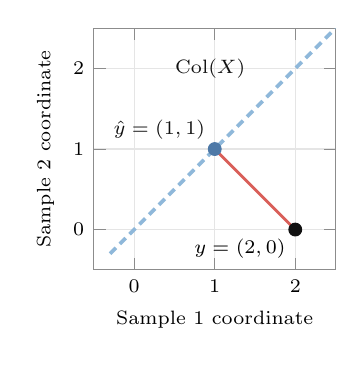
\begin{tikzpicture}
\begin{axis}[
width=4.65cm,
height=4.65cm,
font=\scriptsize,
tick label style={font=\scriptsize},
label style={font=\scriptsize},
axis line style={black!45},
tick style={black!45},
grid=major,
grid style={black!10},
xmin=-0.5,
xmax=2.5,
ymin=-0.5,
ymax=2.5,
xlabel={Sample 1 coordinate},
ylabel={Sample 2 coordinate},
scaled ticks=false,
tick label style={/pgf/number format/fixed},
clip=true,
unbounded coords=jump,
legend style={font=\scriptsize,draw=none,fill=none,at={(0.5,-0.29)},anchor=north,legend cell align=left,column sep=0.12cm,row sep=0.03cm},
legend columns=2,
axis equal image,
xtick={0,1,2},
ytick={0,1,2}
]
\addplot+[no marks,draw=lightplot,line width=1.3pt,densely dashed] coordinates {(-0.3,-0.3) (2.5,2.5)};
\addplot+[no marks,draw=redplot,line width=1pt] coordinates {(1,1) (2,0)};
\addplot+[only marks,mark=*,mark size=2.3pt,draw=inkplot,fill=inkplot,mark options={draw=inkplot,fill=inkplot}] coordinates {(2,0)};
\addplot+[only marks,mark=*,mark size=2.3pt,draw=blueplot,fill=blueplot,mark options={draw=blueplot,fill=blueplot}] coordinates {(1,1)};
\node[anchor=north east,font=\scriptsize] at (axis cs:2,0) {$y=(2,0)$};
\node[anchor=south east,font=\scriptsize,text=inkplot] at (axis cs:1,1) {$\hat y=(1,1)$};
\node[anchor=east,font=\scriptsize,text=inkplot] at (axis cs:1.5,2) {$\operatorname{Col}(X)$};
\end{axis}
\end{tikzpicture}
\endgroup
\end{column}
\begin{column}{0.42\textwidth}\small
The projection of black point $y$ lies in $\Col(X)$.
\[
\widehat y=P_Xy,\qquad
X^{\mathsf T}(y-\widehat y)=0.
\]
The red residual is orthogonal to every feature column.
\end{column}\end{columns}
\vfill
\begin{takeaway}Two-dimensional example: $X=[1,1]^{\mathsf T}$, $y=[2,0]^{\mathsf T}$, $\widehat y=[1,1]^{\mathsf T}$.\end{takeaway}
\end{frame}

% Slide 23 | lsq-26
\begin{frame}{Derive the projection matrix}
\lead{The fitted vector is a linear transformation of the observed responses}
\begin{definitionbox}
\[
\begin{aligned}
\widehat y&=X\widehat\theta=Py,
\qquad P=X(X^{\mathsf T}X)^{-1}X^{\mathsf T},\\
P^{\mathsf T}&=P,\\
P^2&=X(X^{\mathsf T}X)^{-1}(X^{\mathsf T}X)
(X^{\mathsf T}X)^{-1}X^{\mathsf T}=P,\\
PX&=X,\qquad X^{\mathsf T}(I-P)=0.
\end{aligned}
\]
\end{definitionbox}
\small
\begin{itemize}\setlength{\itemsep}{7pt}
\item Assume full column rank here. Symmetry and idempotence identify an orthogonal projection.
\item $P$ preserves vectors in $\Col(X)$ and removes their orthogonal component.
\end{itemize}
\end{frame}

% Slide 24 | lsq-27
\begin{frame}{A Pythagorean proof of the best fit}
\lead{Every competing prediction adds a perpendicular component of error}
\begin{definitionbox}
\[
\begin{aligned}
e&=y-\widehat y,\qquad \widehat y=Py,\qquad z\in\Col(X),\\
y-z&=e+(\widehat y-z),\qquad e^{\mathsf T}(\widehat y-z)=0,\\
\lVert y-z\rVert^2&=\lVert e\rVert^2+\lVert\widehat y-z\rVert^2
\ge\lVert e\rVert^2,\\
\mathbf1\in\Col(X)&\quad\Longrightarrow\quad
\mathbf1^{\mathsf T}e=0\quad\Longrightarrow\quad
\overline{\widehat y}=\bar y.
\end{aligned}
\]
\end{definitionbox}
\small
\begin{itemize}\setlength{\itemsep}{7pt}
\item Equality holds only when the competing fitted vector is $z=\widehat y$.
\item An included intercept makes residuals sum to zero; it does not make residuals independent of inputs.
\end{itemize}
\end{frame}



\SectionSlide{Ill-conditioning and remedies}{}


% Slide 27 | conditioning-28
\begin{frame}{Unique predictions, unique parameters?}
\lead{Can the data distinguish different parameter values?}
\small
\begin{itemize}\setlength{\itemsep}{10pt}
\item \textbf{Full column rank.} $X^{\mathsf T}X$ is positive definite; the OLS parameters are unique.
\item \textbf{Rank deficiency.} There is a $v\ne0$ such that $Xv=0$.
\item \textbf{Indistinguishable.} $\theta$ and $\theta+v$ make identical training predictions.
\item \textbf{Choosing a solution.} The pseudoinverse selects the minimum Euclidean norm.
\end{itemize}
\vfill
\begin{takeaway}More features do not automatically add information. Predictions at new inputs may still differ.\end{takeaway}
\end{frame}

% Slide 28 | conditioning-29
\begin{frame}{The compact singular value decomposition}
\lead{SVD decompostion:}
\begin{definitionbox}
\[
 X=U_r\Sigma_r V_r^{\mathsf T},\qquad r=\rank(X),
 \qquad \Sigma_r=\diag(s_1,\ldots,s_r),
\]
\[
 X\in\R^{n\times p},\quad U_r\in\R^{n\times r},\quad
 V_r\in\R^{p\times r},\quad s_1\geq\cdots\geq s_r>0.
\]
\end{definitionbox}
\small
\begin{itemize}\setlength{\itemsep}{7pt}
\item $U_r^{\mathsf T}U_r=V_r^{\mathsf T}V_r=I_r$: the columns are orthonormal.
\item A parameter direction $v_j$ produces the prediction direction
      $Xv_j=s_j u_j$.
\item Small $s_j$: a large coefficient change can produce a small change in the observed predictions.
\end{itemize}
\end{frame}

% Slide 29 | conditioning-30
\begin{frame}{Least squares in singular coordinates}
\small
Write $\theta=V_r a+v_0$, where $Xv_0=0$, and let $c_j=u_j^{\mathsf T}y$.
\begin{definitionbox}
\[
 \|X\theta-y\|_2^2
 =\sum_{j=1}^r(s_j a_j-c_j)^2
   +\|(I-U_rU_r^{\mathsf T})y\|_2^2.
\]
\[
 \frac{\partial}{\partial a_j}(s_j a_j-c_j)^2
 =2s_j(s_j a_j-c_j)=0
 \quad\Longrightarrow\quad \widehat a_j=\frac{c_j}{s_j}.
\]
\end{definitionbox}
\[
 \widehat\theta_{\min}=\sum_{j=1}^r v_j \cdot\frac{u_j^{\mathsf T}y}{s_j} =\underbrace{V_r\Sigma_r^{-1}U_r^{\mathsf T}}_{X^+}y 
\]
\[ X^+ = (X^{\top}X)^{-1}X^{\top} \text{ when } (X^{\top}X) \text{ is invertible}
\]
\end{frame}

% Slide 30 | conditioning-31
\begin{frame}{Rank deficiency and minimum norm}
\lead{Rank deficiency creates freedom in the coefficients, not in the fitted values}
\begin{definitionbox}
\[
 \underset{\theta}{\argmin}\;\|X\theta-y\|_2^2
 =\{X^+y+v_0:\;v_0\in\ker(X)\}.
\]
\[
 \|X^+y+v_0\|_2^2=\|X^+y\|_2^2+\|v_0\|_2^2,
 \qquad \widehat y=XX^+y.
\]
\end{definitionbox}
\small
\begin{itemize}\setlength{\itemsep}{7pt}
\item $X^+y$ is orthogonal to $\ker(X)$, so $v_0=0$ uniquely minimizes the parameter norm.
\item Every least-squares minimizer has the same training prediction $\widehat y$.
\item Example: $X=[1\;1]$, $y=1$. All $(a,1-a)^{\mathsf T}$ fit exactly; the minimum-norm choice is $(1/2,1/2)^{\mathsf T}$.
\end{itemize}
\end{frame}

% Slide 31 | conditioning-32
\begin{frame}{Collinearity destabilizes coefficients}
\lead{Similar predictions can conceal large coefficient changes}
\begin{columns}[T,onlytextwidth]
\begin{column}{0.55\textwidth}% Generated from work/deck/chart-data-en.mjs; numeric data preserved.
% Input in a column; rocpr is intended for full frame width.
\begingroup
\definecolor{blueplot}{HTML}{4E79A7}
\definecolor{redplot}{HTML}{D95F59}
\definecolor{inkplot}{HTML}{111111}
\definecolor{lightplot}{HTML}{8FB8DA}
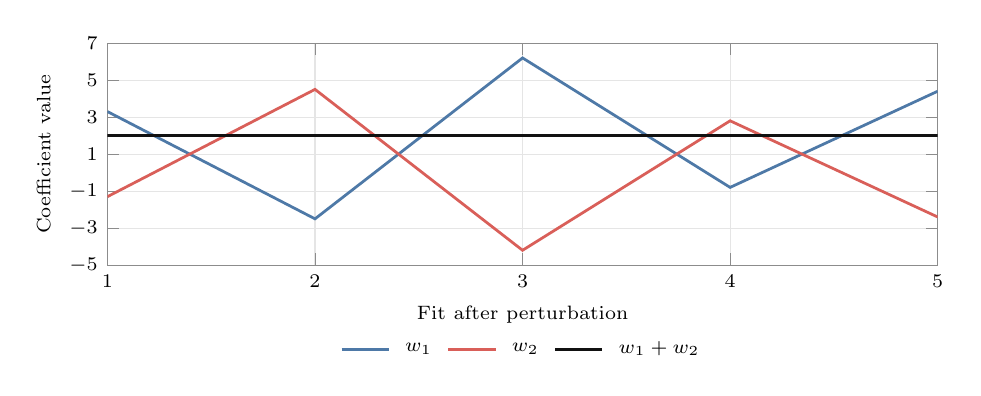
\begin{tikzpicture}
\begin{axis}[
width=\linewidth,
height=4.4cm,
font=\scriptsize,
tick label style={font=\scriptsize},
label style={font=\scriptsize},
axis line style={black!45},
tick style={black!45},
grid=major,
grid style={black!10},
xmin=1,
xmax=5,
ymin=-5,
ymax=7,
xlabel={Fit after perturbation},
ylabel={Coefficient value},
scaled ticks=false,
tick label style={/pgf/number format/fixed},
clip=true,
unbounded coords=jump,
legend style={font=\scriptsize,draw=none,fill=none,at={(0.5,-0.29)},anchor=north,legend cell align=left,column sep=0.12cm,row sep=0.03cm},
legend columns=-1,
xtick={1,2,3,4,5},
ytick={-5,-3,-1,1,3,5,7}
]
\addplot+[no marks,draw=blueplot,line width=1pt] coordinates {(1,3.3) (2,-2.49999999999) (3,6.19999999999) (4,-0.799999999993) (5,4.39999999999)};
\addlegendentry{$w_1$}
\addplot+[no marks,draw=redplot,line width=1pt] coordinates {(1,-1.3) (2,4.49999999999) (3,-4.19999999999) (4,2.79999999999) (5,-2.39999999999)};
\addlegendentry{$w_2$}
\addplot+[no marks,draw=inkplot,line width=1pt] coordinates {(1,2) (2,2) (3,2) (4,2) (5,2)};
\addlegendentry{$w_1+w_2$}
\end{axis}
\end{tikzpicture}
\endgroup
\end{column}
\begin{column}{0.42\textwidth}\small
\begin{itemize}\setlength{\itemsep}{13pt}
\item When $x_2\approx x_1$, the data mainly constrain $w_1+w_2$.
\item Small singular-value directions amplify data noise.
\item Standardization cannot remove genuine collinearity.
\end{itemize}
\end{column}\end{columns}
\end{frame}

% Slide 32 | conditioning-33
\begin{frame}{Full rank does not imply stability}
\lead{Existence and uniqueness are different from sensitivity to perturbations}
\begin{definitionbox}
\[
 \rank(X)=p\quad\Longleftrightarrow\quad s_p>0,
 \qquad \kappa_2(X)=\frac{s_1}{s_p}.
\]
\[
 \Delta\widehat\theta=X^+\Delta y,
 \qquad
 \|\Delta\widehat\theta\|_2\leq\frac{\|\Delta y\|_2}{s_p}
 \quad\text{when $X$ is fixed.}
\]
\end{definitionbox}
\small
\begin{itemize}\setlength{\itemsep}{7pt}
\item Full rank answers whether the coefficients are uniquely determined in exact arithmetic.
\item A large condition number signals very different strengths across parameter directions.
\item Whether sensitivity is unacceptable depends on noise, units, arithmetic precision, and the intended use. There is no universal cutoff.
\end{itemize}
\end{frame}

% Slide 33 | conditioning-34
\begin{frame}{A controlled near-collinear design}
\lead{Two columns become nearly equal while the matrix remains full rank}
\small
Let $q_1,q_2$ be orthonormal. For the concrete two-sample example, use
$q_1=(1,0)^{\mathsf T}$ and $q_2=(0,1)^{\mathsf T}$. 
\begin{definitionbox}
\[
 X_\epsilon=[q_1+\epsilon q_2\;\;q_1-\epsilon q_2]
 =\begin{bmatrix}1&1\\\epsilon&-\epsilon\end{bmatrix},
 \qquad 0<\epsilon\leq1.
\]
\[
 v_+=\frac{1}{\sqrt2}\begin{bmatrix}1\\1\end{bmatrix},\quad
 v_-=\frac{1}{\sqrt2}\begin{bmatrix}1\\-1\end{bmatrix},\quad
 X_\epsilon v_+=\sqrt2q_1,\quad X_\epsilon v_-=\sqrt2\epsilon q_2.
\]
\end{definitionbox}
\[
 s_+=\sqrt2,\qquad s_-=\sqrt2\epsilon,\qquad
 \kappa_2(X_\epsilon)=\epsilon^{-1}.
\]

\end{frame}

% Slide 34 | conditioning-35
\begin{frame}{A tiny response change}
\lead{Keep the design fixed and perturb only its weak response direction}
\begin{definitionbox}
\[
\begin{gathered}
 y=q_1,\qquad y'=q_1+\delta q_2,\qquad
 X_\epsilon\widehat\theta'=y',\\[4pt]
 \widehat\theta_1'+\widehat\theta_2'=1,\qquad
 \epsilon(\widehat\theta_1'-\widehat\theta_2')=\delta.
\end{gathered}
\]
\uncover<2->{\[
 \widehat\theta'=\begin{bmatrix}1/2+\delta/(2\epsilon)\\1/2-\delta/(2\epsilon)\end{bmatrix},
 \qquad \|\Delta\widehat\theta\|_2=\frac{|\delta|}{\sqrt2\epsilon}.
\]}
\end{definitionbox}
\small
\uncover<3->{With $\epsilon=10^{-4}$ and $\delta=10^{-3}$:
\[
 \begin{bmatrix}0.5\\0.5\end{bmatrix}
 \longrightarrow
 \begin{bmatrix}5.5\\-4.5\end{bmatrix},\qquad
 \|\Delta y\|_2=0.001,\quad\|\Delta\widehat\theta\|_2\approx7.071.
\]}
\end{frame}

% Slide 35 | conditioning-36
\begin{frame}{Which predictions remain stable?}
\lead{Coefficient error, training prediction error, and future prediction error differ}
\begin{definitionbox}
\[
 \Delta\widehat y=XX^+\Delta y, \qquad  \|XX^+\|_{\mathrm{op}}\leq 1, 
 \qquad \|\Delta\widehat y\|_2\leq\|\Delta y\|_2.
\]
\[
 \Delta f(x_*)=x_*^{\mathsf T}\Delta\widehat\theta
 =\sum_{j=1}^r\frac{(x_*^{\mathsf T}v_j)(u_j^{\mathsf T}\Delta y)}{s_j}.
\]
\end{definitionbox}
\small
For the controlled example, with $\epsilon=10^{-4}$ and $\delta=10^{-3}$:
{\centering
\begin{tabular}{@{}lll@{}}
\toprule
\textbf{Quantity} & \textbf{Change} & \textbf{Reason}\\\midrule
Training fitted vector & $\delta q_2$ & Norm $0.001$\\
Future input $x_*=(1,1)^{\mathsf T}$ & $0$ & Uses the coefficient sum\\
Future input $x_*=(1,-1)^{\mathsf T}$ & $\delta/\epsilon=10$ & Amplifies the weak direction\\\bottomrule
\end{tabular}
\par}
\vfill
\begin{takeaway}Stable predictions on the observed design do not guarantee stability for a new feature pattern.\end{takeaway}
\note{Suggested time: 5 minutes. The matrix $XX^+$ is an orthogonal projector, whose Euclidean operator norm is at most one. This explains why the fitted training vector can be insensitive in absolute norm even when the coefficients are highly sensitive. The statement holds for fixed $X$ and response perturbations; it is not a universal guarantee about future data or perturbations of the design. To analyze a future input, insert the singular expansion of the coefficient change and inspect its alignment with the weak right singular directions. In our example, the two future vectors respectively isolate the stable sum and the unstable difference. The second vector departs from the near-equality pattern seen at substantial scale in the training data. It is not outside the algebraic span of this full-rank toy design; the issue is that the difference direction was observed only at tiny magnitude. Discuss how this resembles correlated sensors separating after deployment.}
\end{frame}

% Slide 36 | conditioning-37
\begin{frame}{Sampling variance in weak directions}
\lead{The same singular-value division appears in statistical uncertainty}
\small
Fixed $X$ with $\rank(X)=p$: $y=X\theta_*+\xi$, $\E[\xi\mid X]=0$,
and $\Cov(\xi\mid X)=\sigma^2I$.
\begin{definitionbox}
\[
 \widehat\theta-\theta_*
 =\sum_{j=1}^p\frac{u_j^{\mathsf T}\xi}{s_j}v_j,
 \qquad \Cov(\widehat\theta\mid X)
 =\sigma^2 V\diag(s_j^{-2})V^{\mathsf T}.
\]
\[
 \Var(v_j^{\mathsf T}\widehat\theta\mid X)=\frac{\sigma^2}{s_j^2}.
\]
\end{definitionbox}
\small
\begin{itemize}\setlength{\itemsep}{5pt}
\item Tenfold smaller $s_j$ gives hundredfold larger variance; 
\end{itemize}
\end{frame}


% Slide 39 | conditioning-40
\begin{frame}{Numerical rank is a tolerance decision}
\lead{A tiny positive singular value need not contain usable information}
\begin{definitionbox}
\[
 \mathcal I_\tau=\{j:s_j>\tau s_1\},\qquad
 \widehat\theta_\tau=\sum_{j\in\mathcal I_\tau}
       \frac{u_j^{\mathsf T}y}{s_j}v_j,
 \qquad
 \widehat y_\tau=\sum_{j\in\mathcal I_\tau}u_j u_j^{\mathsf T}y.
\]
\end{definitionbox}
\small
\begin{itemize}\setlength{\itemsep}{7pt}
\item Truncated SVD keeps selected singular directions and removes the rest.
\item A roundoff heuristic is $\tau\sim\max(n,p)u$, where $u$ is unit roundoff. Measurement noise may justify stronger truncation.
\item Try-and-error in order: inspect feature scales and singular values; check residuals and solver sensitivity; test the intended future prediction task.
\end{itemize}
\end{frame}


% Slide 41 | conditioning-42
\begin{frame}{Gradient descent for linear regression}

\small Why is Gradient Descent (GD) not the closed-form solution \( X^+ y \)?  
The dimension \( p \) can be large, and the data may arrive in a stream.

\small{Quadratic curvature determines step size and convergence}
\begin{definitionbox}
\[
\begin{gathered}
\theta_{t+1}=\theta_t-\frac{\eta}{n}X^{\mathsf T}(X\theta_t-y),\\
H=\frac{1}{n}X^{\mathsf T}X,\qquad L=\lambda_{\max}(H),\qquad 0<\eta<\frac{2}{L}.
\end{gathered}
\]
\end{definitionbox}
\small
\begin{itemize}\setlength{\itemsep}{8pt}
\item With full column rank, this step size contracts error in every eigendirection.
\item The largest curvature limits the stable step size.
\item The convergence factor is $\max_j\lvert1-\eta\lambda_j\rvert$.
\end{itemize}
\vfill
\begin{takeaway}Derivation: $\theta_{t+1}-\theta^*=(I-\eta H)(\theta_t-\theta^*)$.\end{takeaway}
\note{Suggested time: 4 minutes. For a quadratic objective this is an exact error recursion, not a local approximation. Along eigenvector \(j\) of the Hessian, the error is multiplied by \(1-\eta\lambda_j\). Contraction in every nonzero-curvature direction requires an absolute value below 1, giving \(0<\eta<\frac{2}{L}\). With full column rank, \(H\) is positive definite and the parameters converge to the unique solution. Under rank deficiency, zero-curvature directions do not contract, and the initial null-space component is retained. Gradient methods are motivated by large samples, sparse data, and online updates; we need not assume that the normal equations are always unusable. Over the full interval \(0<\eta<\frac{2}{L}\), the slowest direction is determined by the largest absolute contraction factor. When \(\eta\) exceeds \(\frac{1}{L}\), the largest-eigenvalue direction can become the bottleneck, so the smallest curvature is not unconditionally the slowest direction.\par\medskip\textbf{Further reading.}
\begin{itemize}
\item Tengyu Ma and Andrew Ng, CS229 Lecture Notes, Chapters 1--3 and 8--9. \url{https://cs229.stanford.edu/main_notes.pdf}
\end{itemize}\par\smallskip\textbf{Web demonstration.} \url{https://regression-lab-graduate-2026.whu38f.chatgpt.site/\#gradient-descent}}
\end{frame}

% Slide 42 | conditioning-43
\begin{frame}{Ill-conditioning slows gradient descent}
\lead{A stable step size can still produce very slow progress}
\begin{definitionbox}
\[
\begin{gathered}
e_{t+1}=(I-\eta H)e_t,\qquad H=\frac1nX^{\mathsf T}X,\qquad e_t=\theta_t-\widehat\theta,\\
\eta_* =\frac{2}{L+\mu},\qquad
q_* =\max_j|1-\eta_*\lambda_j(H)|
 =\frac{\kappa_H-1}{\kappa_H+1},\\
\kappa_H=\frac{L}{\mu}=\kappa_2(X)^2,\qquad
\lVert e_t\rVert_2\le q_*^t\lVert e_0\rVert_2.
\end{gathered}
\]
\end{definitionbox}
\small
\begin{itemize}\setlength{\itemsep}{4pt}
\item Assume full column rank, with $0<\mu=\lambda_{\min}(H)\le L$.
\item If $\kappa_2(X)=10^3$, then $\kappa_H=10^6$ and $q_*\approx0.999998$.
\item Diretional rescaling can help improve the efficiency. 
\end{itemize}
\end{frame}

% Slide 43 | conditioning-44
\begin{comment}
\begin{frame}{Feature scale changes optimization}
\lead{The same prediction problem can have very different coordinates}
\begin{columns}[T,onlytextwidth]
\begin{column}{0.55\textwidth}% Generated from work/deck/chart-data-en.mjs; numeric data preserved.
% Input in a column; rocpr is intended for full frame width.
\begingroup
\definecolor{blueplot}{HTML}{4E79A7}
\definecolor{redplot}{HTML}{D95F59}
\definecolor{inkplot}{HTML}{111111}
\definecolor{lightplot}{HTML}{8FB8DA}
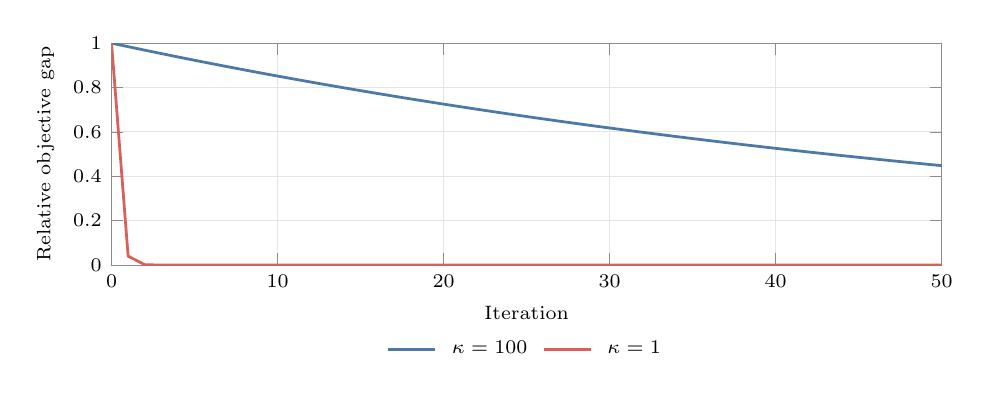
\begin{tikzpicture}
\begin{axis}[
width=\linewidth,
height=4.4cm,
font=\scriptsize,
tick label style={font=\scriptsize},
label style={font=\scriptsize},
axis line style={black!45},
tick style={black!45},
grid=major,
grid style={black!10},
xmin=0,
xmax=50,
ymin=0,
ymax=1,
xlabel={Iteration},
ylabel={Relative objective gap},
scaled ticks=false,
tick label style={/pgf/number format/fixed},
clip=true,
unbounded coords=jump,
legend style={font=\scriptsize,draw=none,fill=none,at={(0.5,-0.29)},anchor=north,legend cell align=left,column sep=0.12cm,row sep=0.03cm},
legend columns=-1,
xtick={0,10,20,30,40,50},
ytick={0,0.2,0.4,0.6,0.8,1}
]
\addplot+[no marks,draw=blueplot,line width=1pt] coordinates {(0,1) (1,0.984064) (2,0.968381956096) (3,0.952949821244) (4,0.937763612892) (5,0.922819411957) (6,0.908113361808) (7,0.893641667275) (8,0.879400593665) (9,0.865386465804) (10,0.851595667085) (11,0.838024638534) (12,0.824669877895) (13,0.811527938721) (14,0.798595429489) (15,0.785869012725) (16,0.773345404138) (17,0.761021371778) (18,0.748893735197) (19,0.736959364633) (20,0.725215180198) (21,0.713658151087) (22,0.702285294791) (23,0.691093676333) (24,0.680080407507) (25,0.669242646133) (26,0.658577595324) (27,0.648082502765) (28,0.637754660001) (29,0.627591401739) (30,0.617590105161) (31,0.607748189245) (32,0.598063114102) (33,0.588532380315) (34,0.579153528302) (35,0.569924137675) (36,0.560841826617) (37,0.551904251268) (38,0.54310910512) (39,0.534454118421) (40,0.52593705759) (41,0.51755572464) (42,0.509307956612) (43,0.501191625016) (44,0.493204635279) (45,0.485344926212) (46,0.477610469468) (47,0.469999269026) (48,0.462509360675) (49,0.455138811503) (50,0.447885719403)};
\addlegendentry{$\kappa=100$}
\addplot+[no marks,draw=redplot,line width=1pt] coordinates {(0,1) (1,0.04) (2,0.0016) (3,0.000064) (4,0.00000256) (5,1.024e-7) (6,4.096e-9) (7,1.6384e-10) (8,6.5536e-12) (9,2.62144e-13) (10,1.048576e-14) (11,4.194304e-16) (12,1.6777216e-17) (13,6.7108864e-19) (14,2.68435456e-20) (15,1.073741824e-21) (16,4.294967296e-23) (17,1.7179869184e-24) (18,6.8719476736e-26) (19,2.74877906944e-27) (20,1.09951162778e-28) (21,4.3980465111e-30) (22,1.75921860444e-31) (23,7.03687441777e-33) (24,2.81474976711e-34) (25,1.12589990684e-35) (26,4.50359962737e-37) (27,1.80143985095e-38) (28,7.20575940379e-40) (29,2.88230376152e-41) (30,1.15292150461e-42) (31,4.61168601843e-44) (32,1.84467440737e-45) (33,7.37869762948e-47) (34,2.95147905179e-48) (35,1.18059162072e-49) (36,4.72236648287e-51) (37,1.88894659315e-52) (38,7.55578637259e-54) (39,3.02231454904e-55) (40,1.20892581961e-56) (41,4.83570327846e-58) (42,1.93428131138e-59) (43,7.73712524553e-61) (44,3.09485009821e-62) (45,1.23794003929e-63) (46,4.95176015714e-65) (47,1.98070406286e-66) (48,7.92281625143e-68) (49,3.16912650057e-69) (50,1.26765060023e-70)};
\addlegendentry{$\kappa=1$}
\end{axis}
\end{tikzpicture}
\endgroup
\end{column}
\begin{column}{0.42\textwidth}\small
\begin{itemize}\setlength{\itemsep}{13pt}
\item Different units can create elongated loss contours.
\item Standardization often makes a fixed step size easier to choose.
\item Estimate scaling parameters from training data only.
\end{itemize}
\end{column}\end{columns}
\end{frame}
\end{comment}
% Slide 44 | remedies
\begin{frame}{Choose the right remedy}
\lead{A reliable computation cannot create information that the data do not contain}
\small\begin{tabularx}{\textwidth}{@{}lYY@{}}\toprule
\textbf{Problem} & \textbf{Response} & \textbf{What changes?}\\\midrule
Inconsistent units & Center and scale & Coordinates; OLS fitted space is preserved\\[3pt]
Avoidable roundoff & QR or SVD solver & Computation of the same LSQ objective\\[3pt]
Weak input directions & Better measurements or a redesigned sample & Information in the data\\[3pt]
Unreliable directions & Truncation, Ridge, or Lasso & Model or objective; bias may increase\\\bottomrule
\end{tabularx}
\end{frame}

% Slide 45 | section-4
\SectionSlide{Regularization: Ridge and Lasso}{}

% Slide 46 | ridge-50
\begin{frame}{Ridge Regression}
\lead{Constrain parameter directions that the data determine poorly}
\begin{definitionbox}
\[
\begin{aligned}
J(\theta;\lambda)&=\frac{\lVert X\theta-y\rVert^2}{2n}+\frac{\lambda}{2}\lVert w\rVert^2,\\
D&=\diag(0,1,\ldots,1),\\
\widehat\theta&=(X^{\mathsf T}X+n\lambda D)^{-1}X^{\mathsf T}y.
\end{aligned}
\]
\end{definitionbox}
\small
\begin{itemize}\setlength{\itemsep}{7pt}
\item $\lambda>0$ shrinks slopes; the intercept is unpenalized.
\item Small singular-value directions receive stronger relative shrinkage.
\item Select $\lambda$ using validation data.
\end{itemize}
\end{frame}

% Slide 47 | ridge-51
\begin{frame}{Ridge filters singular directions}
\lead{Derive the exact shrinkage factors}
\begin{definitionbox}
\[
 \min_w\;\frac{\|X\theta-y\|_2^2}{2n}+\frac{\lambda}{2}\|\theta\|_2^2,
 \qquad X=U_r\diag(s_j)V_r^{\mathsf T}.
\]
\[
 \widehat \theta_\lambda
 =\sum_{j=1}^r\frac{s_j}{s_j^2+n\lambda}(u_j^{\mathsf T}y_c)v_j,
 \qquad
X\widehat \theta_\lambda
 =\sum_{j=1}^r\underbrace{\frac{s_j^2}{s_j^2+n\lambda}}_{h_j}
 (u_j^{\mathsf T}y_c)u_j.
\]
\end{definitionbox}
\small
Model $\theta = \sum_{j} a_j v_j$.
The scalar normal equation is $(s_j^2+n\lambda)a_j=s_j u_j^{\mathsf T}y_c$.
For $\lambda>0$, null-space coefficients are zero.
\end{frame}


% Slide 49 | ridge-53
\begin{frame}{Ridge stabilizes the controlled example}
\lead{Compare stability and training fit under one controlled perturbation}
\small
Return to the \textbf{intercept-free} toy, with $n=2$,
$\epsilon=10^{-4}$, and $y=q_1+10^{-3}q_2$.
\begin{definitionbox}
\[
 \widehat \theta_{1,\lambda}=\frac{1}{2(1+\lambda)}
 +\frac{10^{-3}\epsilon}{2(\epsilon^2+\lambda)},\qquad
 \widehat \theta_{2,\lambda}=\frac{1}{2(1+\lambda)}
 -\frac{10^{-3}\epsilon}{2(\epsilon^2+\lambda)}.
\]
\end{definitionbox}
\small
{\centering
\begin{tabular}{@{}rrrr@{}}
\toprule
$\lambda$ & $\widehat \theta_1$ & $\widehat \theta_2$ & Training MSE\\\midrule
$0$ & $5.500000$ & $-4.500000$ & $0$\\
$10^{-6}$ & $0.549504$ & $0.450495$ & $4.9015\times10^{-7}$\\
$10^{-4}$ & $0.500450$ & $0.499450$ & $5.0490\times10^{-7}$\\\bottomrule
\end{tabular}
\par}
At $\lambda=10^{-4}$: strong direction $h_+\approx0.9999$;
weak direction $h_-\approx10^{-4}$.
\end{frame}



% Slide 51 | lasso-1
\begin{frame}{Lasso Regression}
\lead{Ridge shrinks coefficients; an absolute-value penalty can set them to zero}
\begin{definitionbox}\[
\min_{\theta}\;\frac{\|y-X\theta\|_2^2}{2n}+\lambda\|\theta\|_1,
\qquad \|\theta\|_1=\sum_{j=1}^d|\theta_j|.
\]\end{definitionbox}
\small\begin{itemize}\setlength{\itemsep}{9pt}
\item Assume $n>0$, $\lambda\geq0$; the intercept is unpenalized.
\item Fit centering and scaling on the training fold only.
\end{itemize}
\end{frame}

% Slide 52 | lasso-2
\begin{frame}{Why do corners encourage zeros?}
\lead{Where does the smallest loss contour first touch the constraint?}
\noindent\makebox[\textwidth][c]{% Constructed isotropic squared-loss contours centered at (2,0.4).
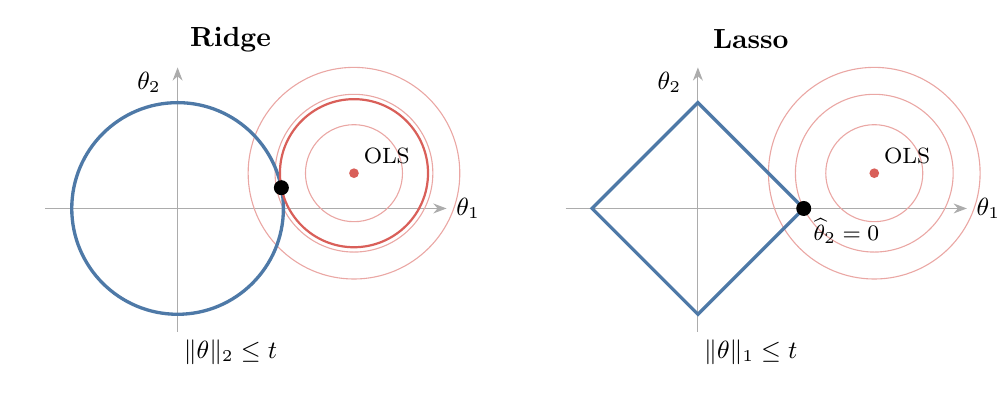
\begin{tikzpicture}[x=1.12cm,y=1.12cm,font=\small]
\path[use as bounding box] (-1.7,-1.85) rectangle (9.1,2.05);
\foreach \shift/\lab in {0/Ridge,5.9/Lasso}{
  \begin{scope}[shift={(\shift,0)}]
  \draw[-{Stealth},gray!65] (-1.5,0)--(3.05,0) node[right,text=black] {$\theta_1$};
  \draw[-{Stealth},gray!65] (0,-1.4)--(0,1.6);
  \node[text=black,anchor=east] at (-.08,1.43) {$\theta_2$};
  \node[font=\bfseries] at (.6,1.92) {\lab};
  \foreach \r in {.55,.894427,1.2}{\draw[redplot!55] (2,.4) circle[radius=\r];}
  \fill[redplot] (2,.4) circle[radius=.055];
  \node[above right,font=\footnotesize] at (2,.4) {OLS};
  \end{scope}
}
\draw[blueplot,very thick] (0,0) circle[radius=1.2];
\draw[blueplot,very thick] (7.1,0)--(5.9,1.2)--(4.7,0)--(5.9,-1.2)--cycle;
\node at (.6,-1.63) {$\|\theta\|_2\leq t$};
\node at (6.5,-1.63) {$\|\theta\|_1\leq t$};
\only<2->{
  \draw[redplot,thick] (2,.4) circle[radius=.839608];
  \fill[black] (1.176697,.235339) circle[radius=.085];
  \fill[black] (7.1,0) circle[radius=.085];
  \node[below right,font=\footnotesize] at (7.1,0) {$\widehat \theta_2=0$};
}
\end{tikzpicture}
}\par
\small\centering Constructed contours; both constraint radii use $t=1.2$.
\vfill\uncover<2->{\begin{takeaway}The $L_1$ boundary has axis-aligned corners; a contact at a corner gives a zero coefficient.\end{takeaway}}
\note{Suggested time: 4 minutes. Build 1: show squared-loss contours centered at the unconstrained estimate (2,0.4) and ask students to predict the first point of contact as the contours expand. Wait 15 seconds. Build 2: reveal the contact points. In this isotropic example, the L2 ball projects the estimate radially to approximately (1.1767,0.2353), while projection onto the L1 ball gives (1.2,0). The latter is a corner, hence an exact zero. Both sets have radius parameter 1.2, but they are different constraints and do not produce the same fit. This is constrained geometry: minimizing squared loss subject to a norm bound. Suitable penalty and constraint parameters can describe the same optimum, but t is not lambda and should not be substituted for it. A corner makes sparse optima possible; the statement is not that every Lasso optimum lies at a corner. An optimum can also lie on an edge with several nonzero coefficients.}
\end{frame}

% Slide 53 | lasso-3
\begin{frame}{Optimality at a zero coefficient}
\lead{At a kink, optimality uses a set of possible slopes}
\begin{definitionbox}\[
\partial|u|=\begin{cases}\{1\},&u>0,\\[-1pt][-1,1],&u=0,\\[-1pt]\{-1\},&u<0,\end{cases}
\qquad
0\in-\frac{X_{j}^{\mathsf T}(y-X\widehat \theta)}{n}
       +\lambda\partial|\widehat \theta_j|.
\]\[
\widehat \theta_j=0\ \Longrightarrow\
\left|\frac{X_j^{\mathsf T}(y-X\widehat \theta)}{n}\right|\leq\lambda.
\]\end{definitionbox}
\small\begin{itemize}\setlength{\itemsep}{9pt}
\item A nonzero coefficient requires residual correlation $=\lambda\,\mathrm{sign}(\widehat \theta_j)$.
\item Convexity makes the full set of these conditions sufficient for a global minimum.
\end{itemize}
\end{frame}



% Slide 55 | lasso-5
\begin{frame}{Deriving a coordinate-descent update}
\lead{Hold the other coefficients fixed; subtract their current predictions}
\begin{definitionbox}\[
r_{-j}=y-\sum_{k\ne j}X_k\theta_k,\qquad
a_j=\frac{\|X_{j}\|_2^2}{n}>0,\quad c_j=\frac{X_j^{\mathsf T}r_{-j}}{n}.
\]\[
\frac{\|r_{-j}-X_j\theta_j\|_2^2}{2n}+\lambda|\theta_j|
=\frac{a_j}{2}\theta_j^2-c_j\theta_j+\lambda|\theta_j|+\text{constant},
\]\end{definitionbox}
\small\begin{itemize}\setlength{\itemsep}{3pt}
\item With our standardization, $a_j=1$; cycle through all retained columns.
\item Use warm starts along a decreasing $\lambda$ sequence; stop using an optimality tolerance.
\end{itemize}
\end{frame}

% Slide 56 | lasso-6
\begin{frame}{Ridge and Lasso trace different paths}
\lead{Constructed normalized orthogonal design: $c=(2,0.8,-0.35)^{\mathsf T}$}
\begin{overlayarea}{\textwidth}{4.85cm}
\only<1>{\vspace{1.1cm}\centering\Large Increase $\lambda$ from zero.\par\bigskip
\large Which coefficients reach exactly zero?}
\only<2>{\begin{minipage}{.48\linewidth}
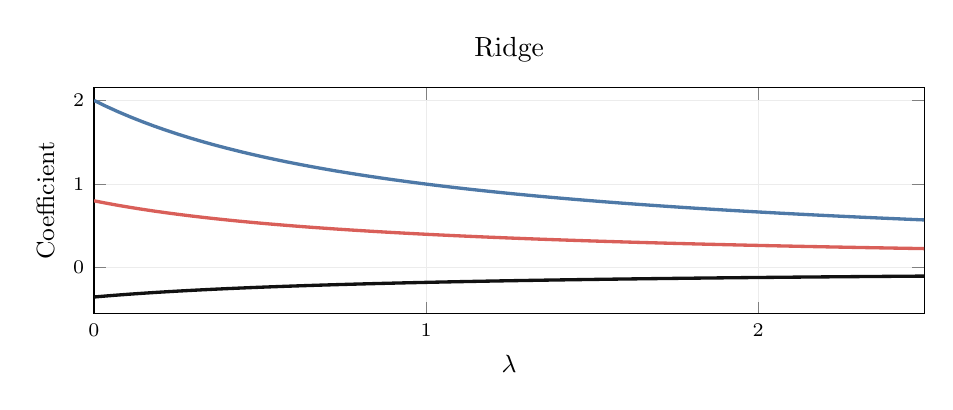
\begin{tikzpicture}
\begin{axis}[width=\linewidth,height=4.45cm,title={Ridge},xmin=0,xmax=2.5,ymin=-.55,ymax=2.15,
  xlabel={$\lambda$},ylabel={Coefficient},xtick={0,1,2},ytick={0,1,2},
  ticklabel style={font=\scriptsize},label style={font=\small},grid=major,grid style={gray!15}]
\addplot[blueplot,very thick,domain=0:2.5,samples=70] {2/(1+x)};
\addplot[redplot,very thick,domain=0:2.5,samples=70] {.8/(1+x)};
\addplot[inkplot,very thick,domain=0:2.5,samples=70] {-.35/(1+x)};
\end{axis}\end{tikzpicture}
\end{minipage}\hfill
\begin{minipage}{.48\linewidth}
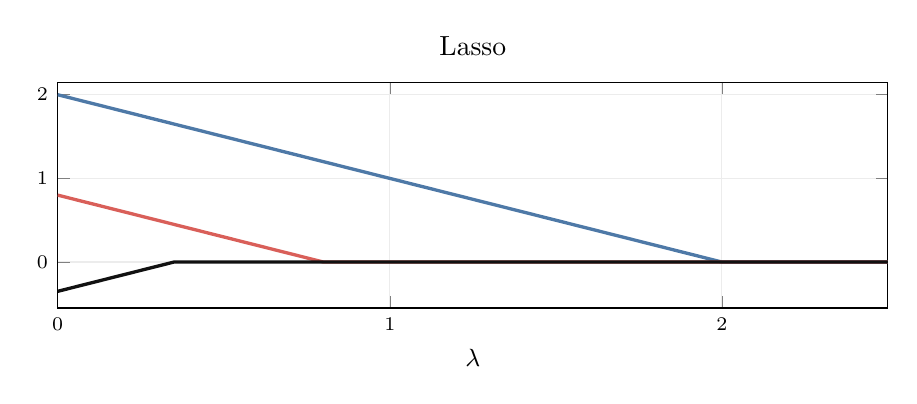
\begin{tikzpicture}
\begin{axis}[width=\linewidth,height=4.45cm,title={Lasso},xmin=0,xmax=2.5,ymin=-.55,ymax=2.15,
  xlabel={$\lambda$},xtick={0,1,2},ytick={0,1,2},
  ticklabel style={font=\scriptsize},label style={font=\small},grid=major,grid style={gray!15}]
\addplot[blueplot,very thick] coordinates {(0,2)(2,0)(2.5,0)};
\addplot[redplot,very thick] coordinates {(0,.8)(.8,0)(2.5,0)};
\addplot[inkplot,very thick] coordinates {(0,-.35)(.35,0)(2.5,0)};
\end{axis}\end{tikzpicture}
\end{minipage}
\par\centering\scriptsize
\textcolor{blueplot}{$w_1$}\qquad\textcolor{redplot}{$w_2$}\qquad\textcolor{inkplot}{$w_3$}
}
\end{overlayarea}\vfill
\uncover<2->{\begin{takeaway}Ridge: $\widehat \theta_j=c_j/(1+\lambda)$.\qquad Lasso: $\widehat \theta_j$: no closed form solution.\end{takeaway}}
\note{Suggested time: 4 minutes. Build 1: ask students to predict the qualitative coefficient paths and pause for 15 seconds. Build 2: reveal two exact analytic examples, not paths estimated from a claimed real dataset. The normalized orthogonal feature design makes both formulas explicit. Ridge divides each nonzero coefficient by one plus lambda and approaches zero continuously without reaching it at a finite penalty in this example. Lasso reaches zero at the coefficient's absolute unpenalized value, so the three knots occur at 0.35, 0.8, and 2. The red and black paths eventually share the horizontal axis; this overlap is intentional. General correlated Lasso paths can enter and leave the active set, so this simple ordering is not a universal rule. The same numerical lambda in the two penalties is not a claim of equal complexity or equal predictive performance. Choose each model's tuning parameter by validation.}
\end{frame}



% Slide 58 | lasso-8
\begin{frame}{Choose a penalty for the modeling task}
\lead{What tradeoff are we willing to make?}
\small\begin{tabularx}{\textwidth}{@{}lYY@{}}\toprule
 & \textbf{Ridge} & \textbf{Lasso}\\\midrule
Penalty & $\lambda\|\theta\|_2^2/2$ & $\lambda\|\theta\|_1$\\[4pt]
Typical behavior & Continuous shrinkage & Shrinkage with possible exact zeros\\[4pt]
Useful preference & Many small effects; stable prediction & A smaller feature set\\[4pt]
Correlated inputs & Spreads weight across similar columns & Selection can be unstable\\[4pt]
Tuning & Validation / cross-validation & Validation / cross-validation\\\bottomrule
\end{tabularx}
\end{frame}


% Slide 60 | section-5
\SectionSlide{Feature expansion: polynomials and kernels}{}
% Slide 61 | features-1
\begin{frame}{Can a linear model bend?}
\lead{5. Feature expansion \hfill Same fitting machinery. Richer inputs.}
\begin{columns}[c,onlytextwidth]
\begin{column}{.54\textwidth}% Native PGFPlots; generated numeric teaching data.
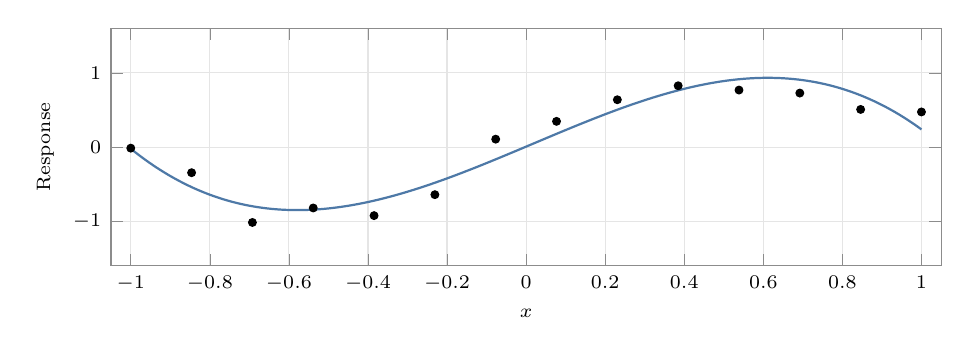
\begin{tikzpicture}
\begin{axis}[width=\linewidth,height=4.6cm,font=\scriptsize,
tick label style={font=\scriptsize},label style={font=\scriptsize},
axis line style={black!45},tick style={black!45},grid=major,grid style={black!10},
scaled ticks=false,xlabel={$x$},ylabel={Response},xmin=-1.05,xmax=1.05,
ymin=-1.6,ymax=1.6,clip=true,unbounded coords=jump,]
\addplot[only marks,mark=*,mark size=1.4pt,black] coordinates {(-1,-0.014539702) (-0.84615385,-0.34516883) (-0.69230769,-1.0151104) (-0.53846154,-0.82009194) (-0.38461538,-0.92297015) (-0.23076923,-0.64102463) (-0.076923077,0.10647764) (0.076923077,0.3460617) (0.23076923,0.63699851) (0.38461538,0.82531436) (0.53846154,0.76750888) (0.69230769,0.72707693) (0.84615385,0.50661061) (1,0.47271884)};
\addplot[no marks,blueplot,thick] coordinates {(-1,-0.022197591) (-0.98888889,-0.069190287) (-0.97777778,-0.11460975) (-0.96666667,-0.15847338) (-0.95555556,-0.20079856) (-0.94444444,-0.2416027) (-0.93333333,-0.28090318) (-0.92222222,-0.3187174) (-0.91111111,-0.35506275) (-0.9,-0.38995663) (-0.88888889,-0.42341644) (-0.87777778,-0.45545955) (-0.86666667,-0.48610338) (-0.85555556,-0.51536531) (-0.84444444,-0.54326274) (-0.83333333,-0.56981306) (-0.82222222,-0.59503366) (-0.81111111,-0.61894195) (-0.8,-0.6415553) (-0.78888889,-0.66289113) (-0.77777778,-0.68296682) (-0.76666667,-0.70179976) (-0.75555556,-0.71940735) (-0.74444444,-0.73580699) (-0.73333333,-0.75101607) (-0.72222222,-0.76505197) (-0.71111111,-0.77793211) (-0.7,-0.78967386) (-0.68888889,-0.80029463) (-0.67777778,-0.80981181) (-0.66666667,-0.81824278) (-0.65555556,-0.82560496) (-0.64444444,-0.83191572) (-0.63333333,-0.83719247) (-0.62222222,-0.8414526) (-0.61111111,-0.8447135) (-0.6,-0.84699257) (-0.58888889,-0.8483072) (-0.57777778,-0.84867478) (-0.56666667,-0.84811271) (-0.55555556,-0.84663839) (-0.54444444,-0.8442692) (-0.53333333,-0.84102254) (-0.52222222,-0.8369158) (-0.51111111,-0.83196639) (-0.5,-0.82619169) (-0.48888889,-0.81960909) (-0.47777778,-0.812236) (-0.46666667,-0.8040898) (-0.45555556,-0.79518789) (-0.44444444,-0.78554767) (-0.43333333,-0.77518652) (-0.42222222,-0.76412184) (-0.41111111,-0.75237103) (-0.4,-0.73995148) (-0.38888889,-0.72688058) (-0.37777778,-0.71317573) (-0.36666667,-0.69885432) (-0.35555556,-0.68393375) (-0.34444444,-0.6684314) (-0.33333333,-0.65236468) (-0.32222222,-0.63575098) (-0.31111111,-0.61860769) (-0.3,-0.6009522) (-0.28888889,-0.58280192) (-0.27777778,-0.56417423) (-0.26666667,-0.54508652) (-0.25555556,-0.5255562) (-0.24444444,-0.50560066) (-0.23333333,-0.48523728) (-0.22222222,-0.46448347) (-0.21111111,-0.44335662) (-0.2,-0.42187412) (-0.18888889,-0.40005337) (-0.17777778,-0.37791175) (-0.16666667,-0.35546668) (-0.15555556,-0.33273553) (-0.14444444,-0.3097357) (-0.13333333,-0.28648459) (-0.12222222,-0.26299959) (-0.11111111,-0.23929809) (-0.1,-0.2153975) (-0.088888889,-0.19131519) (-0.077777778,-0.16706857) (-0.066666667,-0.14267504) (-0.055555556,-0.11815198) (-0.044444444,-0.093516785) (-0.033333333,-0.068786856) (-0.022222222,-0.043979584) (-0.011111111,-0.019112363) (0,0.0057974129) (0.011111111,0.030732349) (0.022222222,0.055675053) (0.033333333,0.080608128) (0.044444444,0.10551418) (0.055555556,0.13037582) (0.066666667,0.15517565) (0.077777778,0.17989628) (0.088888889,0.20452031) (0.1,0.22903034) (0.11111111,0.25340899) (0.12222222,0.27763886) (0.13333333,0.30170256) (0.14444444,0.32558269) (0.15555556,0.34926186) (0.16666667,0.37272267) (0.17777778,0.39594773) (0.18888889,0.41891965) (0.2,0.44162103) (0.21111111,0.46403448) (0.22222222,0.4861426) (0.23333333,0.507928) (0.24444444,0.52937329) (0.25555556,0.55046107) (0.26666667,0.57117395) (0.27777778,0.59149453) (0.28888889,0.61140542) (0.3,0.63088922) (0.31111111,0.64992855) (0.32222222,0.668506) (0.33333333,0.68660419) (0.34444444,0.70420572) (0.35555556,0.72129319) (0.36666667,0.73784921) (0.37777778,0.75385639) (0.38888889,0.76929733) (0.4,0.78415465) (0.41111111,0.79841093) (0.42222222,0.8120488) (0.43333333,0.82505086) (0.44444444,0.83739971) (0.45555556,0.84907795) (0.46666667,0.8600682) (0.47777778,0.87035307) (0.48888889,0.87991515) (0.5,0.88873705) (0.51111111,0.89680138) (0.52222222,0.90409074) (0.53333333,0.91058775) (0.54444444,0.916275) (0.55555556,0.92113511) (0.56666667,0.92515067) (0.57777778,0.92830429) (0.58888889,0.93057859) (0.6,0.93195617) (0.61111111,0.93241962) (0.62222222,0.93195156) (0.63333333,0.9305346) (0.64444444,0.92815134) (0.65555556,0.92478438) (0.66666667,0.92041634) (0.67777778,0.91502981) (0.68888889,0.90860741) (0.7,0.90113174) (0.71111111,0.8925854) (0.72222222,0.882951) (0.73333333,0.87221115) (0.74444444,0.86034846) (0.75555556,0.84734552) (0.76666667,0.83318495) (0.77777778,0.81784936) (0.78888889,0.80132134) (0.8,0.7835835) (0.81111111,0.76461845) (0.82222222,0.7444088) (0.83333333,0.72293714) (0.84444444,0.7001861) (0.85555556,0.67613827) (0.86666667,0.65077626) (0.87777778,0.62408267) (0.88888889,0.59604011) (0.9,0.56663119) (0.91111111,0.53583851) (0.92222222,0.50364469) (0.93333333,0.47003231) (0.94444444,0.434984) (0.95555556,0.39848235) (0.96666667,0.36050998) (0.97777778,0.32104949) (0.98888889,0.28008347) (1,0.23759455)};
\end{axis}
\end{tikzpicture}
\end{column}
\begin{column}{.42\textwidth}
\begin{definitionbox}
\[
\widehat y=b+w_1x+w_2x^2+w_3x^3
\]
\[
\phi(x)=\begin{bmatrix}x&x^2&x^3\end{bmatrix}^{\mathsf T}
\]
\[
\widehat y=b+w^{\mathsf T}\phi(x)
\]
\end{definitionbox}
\medskip\large Linear in $w$.\par\medskip
Curved in $x$.
\end{column}
\end{columns}
\vfill
\begin{takeaway}Feature design changes the functions we can fit.\end{takeaway}
\note{Suggested time: 2 minutes. Ask which object must enter linearly for a model to be called linear regression: the raw input or the unknown coefficients? The cubic curve is still linear in its coefficients. The intercept is separate, so the displayed feature vector excludes a constant. The constructed observations use 14 equally spaced x values on [-1,1], a mean 0.7 sin(pi x)+0.25x, and fixed pseudo-random normal deviations with standard deviation 0.16. A cubic least-squares fit is shown. The plot is a teaching example, not a physical law. Any fixed feature map can replace raw inputs in the design matrix; least squares, ridge, and Lasso can all be applied to the resulting columns. Reference for the feature-map viewpoint: Ng and Ma, Stanford CS229 kernel notes, section 1.1, \url{https://cs229.stanford.edu/summer2019/cs229-notes3.pdf}.}
\end{frame}

% Slide 62 | features-2
\begin{frame}{How much curvature is useful?}
\lead{Fourteen training observations. Which degree would you choose?}
\begin{columns}[c,onlytextwidth]
\begin{column}{.56\textwidth}% Native PGFPlots; generated numeric teaching data.
\begin{tikzpicture}
\begin{axis}[width=\linewidth,height=4.6cm,font=\scriptsize,
tick label style={font=\scriptsize},label style={font=\scriptsize},
axis line style={black!45},tick style={black!45},grid=major,grid style={black!10},
scaled ticks=false,xlabel={$x$},ylabel={Response},xmin=-1.05,xmax=1.05,
ymin=-1.6,ymax=1.6,clip=true,unbounded coords=jump,]
\only<2->{\addplot[no marks,lightplot,thick,dashed] coordinates {(-1,-0.7451799) (-0.98888889,-0.73640024) (-0.97777778,-0.72762057) (-0.96666667,-0.7188409) (-0.95555556,-0.71006123) (-0.94444444,-0.70128157) (-0.93333333,-0.6925019) (-0.92222222,-0.68372223) (-0.91111111,-0.67494257) (-0.9,-0.6661629) (-0.88888889,-0.65738323) (-0.87777778,-0.64860357) (-0.86666667,-0.6398239) (-0.85555556,-0.63104423) (-0.84444444,-0.62226456) (-0.83333333,-0.6134849) (-0.82222222,-0.60470523) (-0.81111111,-0.59592556) (-0.8,-0.5871459) (-0.78888889,-0.57836623) (-0.77777778,-0.56958656) (-0.76666667,-0.56080689) (-0.75555556,-0.55202723) (-0.74444444,-0.54324756) (-0.73333333,-0.53446789) (-0.72222222,-0.52568823) (-0.71111111,-0.51690856) (-0.7,-0.50812889) (-0.68888889,-0.49934923) (-0.67777778,-0.49056956) (-0.66666667,-0.48178989) (-0.65555556,-0.47301022) (-0.64444444,-0.46423056) (-0.63333333,-0.45545089) (-0.62222222,-0.44667122) (-0.61111111,-0.43789156) (-0.6,-0.42911189) (-0.58888889,-0.42033222) (-0.57777778,-0.41155255) (-0.56666667,-0.40277289) (-0.55555556,-0.39399322) (-0.54444444,-0.38521355) (-0.53333333,-0.37643389) (-0.52222222,-0.36765422) (-0.51111111,-0.35887455) (-0.5,-0.35009489) (-0.48888889,-0.34131522) (-0.47777778,-0.33253555) (-0.46666667,-0.32375588) (-0.45555556,-0.31497622) (-0.44444444,-0.30619655) (-0.43333333,-0.29741688) (-0.42222222,-0.28863722) (-0.41111111,-0.27985755) (-0.4,-0.27107788) (-0.38888889,-0.26229822) (-0.37777778,-0.25351855) (-0.36666667,-0.24473888) (-0.35555556,-0.23595921) (-0.34444444,-0.22717955) (-0.33333333,-0.21839988) (-0.32222222,-0.20962021) (-0.31111111,-0.20084055) (-0.3,-0.19206088) (-0.28888889,-0.18328121) (-0.27777778,-0.17450154) (-0.26666667,-0.16572188) (-0.25555556,-0.15694221) (-0.24444444,-0.14816254) (-0.23333333,-0.13938288) (-0.22222222,-0.13060321) (-0.21111111,-0.12182354) (-0.2,-0.11304388) (-0.18888889,-0.10426421) (-0.17777778,-0.095484541) (-0.16666667,-0.086704874) (-0.15555556,-0.077925207) (-0.14444444,-0.06914554) (-0.13333333,-0.060365873) (-0.12222222,-0.051586206) (-0.11111111,-0.042806539) (-0.1,-0.034026872) (-0.088888889,-0.025247205) (-0.077777778,-0.016467538) (-0.066666667,-0.0076878706) (-0.055555556,0.0010917965) (-0.044444444,0.0098714635) (-0.033333333,0.018651131) (-0.022222222,0.027430798) (-0.011111111,0.036210465) (0,0.044990132) (0.011111111,0.053769799) (0.022222222,0.062549466) (0.033333333,0.071329133) (0.044444444,0.0801088) (0.055555556,0.088888467) (0.066666667,0.097668134) (0.077777778,0.1064478) (0.088888889,0.11522747) (0.1,0.12400714) (0.11111111,0.1327868) (0.12222222,0.14156647) (0.13333333,0.15034614) (0.14444444,0.1591258) (0.15555556,0.16790547) (0.16666667,0.17668514) (0.17777778,0.1854648) (0.18888889,0.19424447) (0.2,0.20302414) (0.21111111,0.21180381) (0.22222222,0.22058347) (0.23333333,0.22936314) (0.24444444,0.23814281) (0.25555556,0.24692247) (0.26666667,0.25570214) (0.27777778,0.26448181) (0.28888889,0.27326148) (0.3,0.28204114) (0.31111111,0.29082081) (0.32222222,0.29960048) (0.33333333,0.30838014) (0.34444444,0.31715981) (0.35555556,0.32593948) (0.36666667,0.33471914) (0.37777778,0.34349881) (0.38888889,0.35227848) (0.4,0.36105815) (0.41111111,0.36983781) (0.42222222,0.37861748) (0.43333333,0.38739715) (0.44444444,0.39617681) (0.45555556,0.40495648) (0.46666667,0.41373615) (0.47777778,0.42251581) (0.48888889,0.43129548) (0.5,0.44007515) (0.51111111,0.44885482) (0.52222222,0.45763448) (0.53333333,0.46641415) (0.54444444,0.47519382) (0.55555556,0.48397348) (0.56666667,0.49275315) (0.57777778,0.50153282) (0.58888889,0.51031249) (0.6,0.51909215) (0.61111111,0.52787182) (0.62222222,0.53665149) (0.63333333,0.54543115) (0.64444444,0.55421082) (0.65555556,0.56299049) (0.66666667,0.57177015) (0.67777778,0.58054982) (0.68888889,0.58932949) (0.7,0.59810916) (0.71111111,0.60688882) (0.72222222,0.61566849) (0.73333333,0.62444816) (0.74444444,0.63322782) (0.75555556,0.64200749) (0.76666667,0.65078716) (0.77777778,0.65956683) (0.78888889,0.66834649) (0.8,0.67712616) (0.81111111,0.68590583) (0.82222222,0.69468549) (0.83333333,0.70346516) (0.84444444,0.71224483) (0.85555556,0.72102449) (0.86666667,0.72980416) (0.87777778,0.73858383) (0.88888889,0.7473635) (0.9,0.75614316) (0.91111111,0.76492283) (0.92222222,0.7737025) (0.93333333,0.78248216) (0.94444444,0.79126183) (0.95555556,0.8000415) (0.96666667,0.80882117) (0.97777778,0.81760083) (0.98888889,0.8263805) (1,0.83516017)};
}
\only<2->{\addplot[no marks,blueplot,thick] coordinates {(-1,-0.022197591) (-0.98888889,-0.069190287) (-0.97777778,-0.11460975) (-0.96666667,-0.15847338) (-0.95555556,-0.20079856) (-0.94444444,-0.2416027) (-0.93333333,-0.28090318) (-0.92222222,-0.3187174) (-0.91111111,-0.35506275) (-0.9,-0.38995663) (-0.88888889,-0.42341644) (-0.87777778,-0.45545955) (-0.86666667,-0.48610338) (-0.85555556,-0.51536531) (-0.84444444,-0.54326274) (-0.83333333,-0.56981306) (-0.82222222,-0.59503366) (-0.81111111,-0.61894195) (-0.8,-0.6415553) (-0.78888889,-0.66289113) (-0.77777778,-0.68296682) (-0.76666667,-0.70179976) (-0.75555556,-0.71940735) (-0.74444444,-0.73580699) (-0.73333333,-0.75101607) (-0.72222222,-0.76505197) (-0.71111111,-0.77793211) (-0.7,-0.78967386) (-0.68888889,-0.80029463) (-0.67777778,-0.80981181) (-0.66666667,-0.81824278) (-0.65555556,-0.82560496) (-0.64444444,-0.83191572) (-0.63333333,-0.83719247) (-0.62222222,-0.8414526) (-0.61111111,-0.8447135) (-0.6,-0.84699257) (-0.58888889,-0.8483072) (-0.57777778,-0.84867478) (-0.56666667,-0.84811271) (-0.55555556,-0.84663839) (-0.54444444,-0.8442692) (-0.53333333,-0.84102254) (-0.52222222,-0.8369158) (-0.51111111,-0.83196639) (-0.5,-0.82619169) (-0.48888889,-0.81960909) (-0.47777778,-0.812236) (-0.46666667,-0.8040898) (-0.45555556,-0.79518789) (-0.44444444,-0.78554767) (-0.43333333,-0.77518652) (-0.42222222,-0.76412184) (-0.41111111,-0.75237103) (-0.4,-0.73995148) (-0.38888889,-0.72688058) (-0.37777778,-0.71317573) (-0.36666667,-0.69885432) (-0.35555556,-0.68393375) (-0.34444444,-0.6684314) (-0.33333333,-0.65236468) (-0.32222222,-0.63575098) (-0.31111111,-0.61860769) (-0.3,-0.6009522) (-0.28888889,-0.58280192) (-0.27777778,-0.56417423) (-0.26666667,-0.54508652) (-0.25555556,-0.5255562) (-0.24444444,-0.50560066) (-0.23333333,-0.48523728) (-0.22222222,-0.46448347) (-0.21111111,-0.44335662) (-0.2,-0.42187412) (-0.18888889,-0.40005337) (-0.17777778,-0.37791175) (-0.16666667,-0.35546668) (-0.15555556,-0.33273553) (-0.14444444,-0.3097357) (-0.13333333,-0.28648459) (-0.12222222,-0.26299959) (-0.11111111,-0.23929809) (-0.1,-0.2153975) (-0.088888889,-0.19131519) (-0.077777778,-0.16706857) (-0.066666667,-0.14267504) (-0.055555556,-0.11815198) (-0.044444444,-0.093516785) (-0.033333333,-0.068786856) (-0.022222222,-0.043979584) (-0.011111111,-0.019112363) (0,0.0057974129) (0.011111111,0.030732349) (0.022222222,0.055675053) (0.033333333,0.080608128) (0.044444444,0.10551418) (0.055555556,0.13037582) (0.066666667,0.15517565) (0.077777778,0.17989628) (0.088888889,0.20452031) (0.1,0.22903034) (0.11111111,0.25340899) (0.12222222,0.27763886) (0.13333333,0.30170256) (0.14444444,0.32558269) (0.15555556,0.34926186) (0.16666667,0.37272267) (0.17777778,0.39594773) (0.18888889,0.41891965) (0.2,0.44162103) (0.21111111,0.46403448) (0.22222222,0.4861426) (0.23333333,0.507928) (0.24444444,0.52937329) (0.25555556,0.55046107) (0.26666667,0.57117395) (0.27777778,0.59149453) (0.28888889,0.61140542) (0.3,0.63088922) (0.31111111,0.64992855) (0.32222222,0.668506) (0.33333333,0.68660419) (0.34444444,0.70420572) (0.35555556,0.72129319) (0.36666667,0.73784921) (0.37777778,0.75385639) (0.38888889,0.76929733) (0.4,0.78415465) (0.41111111,0.79841093) (0.42222222,0.8120488) (0.43333333,0.82505086) (0.44444444,0.83739971) (0.45555556,0.84907795) (0.46666667,0.8600682) (0.47777778,0.87035307) (0.48888889,0.87991515) (0.5,0.88873705) (0.51111111,0.89680138) (0.52222222,0.90409074) (0.53333333,0.91058775) (0.54444444,0.916275) (0.55555556,0.92113511) (0.56666667,0.92515067) (0.57777778,0.92830429) (0.58888889,0.93057859) (0.6,0.93195617) (0.61111111,0.93241962) (0.62222222,0.93195156) (0.63333333,0.9305346) (0.64444444,0.92815134) (0.65555556,0.92478438) (0.66666667,0.92041634) (0.67777778,0.91502981) (0.68888889,0.90860741) (0.7,0.90113174) (0.71111111,0.8925854) (0.72222222,0.882951) (0.73333333,0.87221115) (0.74444444,0.86034846) (0.75555556,0.84734552) (0.76666667,0.83318495) (0.77777778,0.81784936) (0.78888889,0.80132134) (0.8,0.7835835) (0.81111111,0.76461845) (0.82222222,0.7444088) (0.83333333,0.72293714) (0.84444444,0.7001861) (0.85555556,0.67613827) (0.86666667,0.65077626) (0.87777778,0.62408267) (0.88888889,0.59604011) (0.9,0.56663119) (0.91111111,0.53583851) (0.92222222,0.50364469) (0.93333333,0.47003231) (0.94444444,0.434984) (0.95555556,0.39848235) (0.96666667,0.36050998) (0.97777778,0.32104949) (0.98888889,0.28008347) (1,0.23759455)};
}
\only<2->{\addplot[no marks,redplot,thick] coordinates {(-1,-0.014569741) (-0.98888889,0.43218702) (-0.97777778,0.72653794) (-0.96666667,0.89650204) (-0.95555556,0.96663205) (-0.94444444,0.95829789) (-0.93333333,0.88995891) (-0.92222222,0.77742449) (-0.91111111,0.63410239) (-0.9,0.47123452) (-0.88888889,0.29811981) (-0.87777778,0.12232415) (-0.86666667,-0.050122721) (-0.85555556,-0.21454329) (-0.84444444,-0.36744118) (-0.83333333,-0.50634267) (-0.82222222,-0.62965063) (-0.81111111,-0.73651044) (-0.8,-0.82668763) (-0.78888889,-0.90045677) (-0.77777778,-0.95850115) (-0.76666667,-1.0018228) (-0.75555556,-1.0316624) (-0.74444444,-1.0494285) (-0.73333333,-1.0566357) (-0.72222222,-1.0548503) (-0.71111111,-1.0456455) (-0.7,-1.0305612) (-0.68888889,-1.0110732) (-0.67777778,-0.98856621) (-0.66666667,-0.96431396) (-0.65555556,-0.93946378) (-0.64444444,-0.91502587) (-0.63333333,-0.89186673) (-0.62222222,-0.87070625) (-0.61111111,-0.85211795) (-0.6,-0.8365321) (-0.58888889,-0.82424112) (-0.57777778,-0.81540708) (-0.56666667,-0.81007078) (-0.55555556,-0.80816215) (-0.54444444,-0.80951167) (-0.53333333,-0.81386249) (-0.52222222,-0.820883) (-0.51111111,-0.83017957) (-0.5,-0.84130931) (-0.48888889,-0.85379265) (-0.47777778,-0.86712545) (-0.46666667,-0.88079068) (-0.45555556,-0.89426934) (-0.44444444,-0.90705072) (-0.43333333,-0.91864166) (-0.42222222,-0.92857502) (-0.41111111,-0.93641708) (-0.4,-0.94177391) (-0.38888889,-0.94429677) (-0.37777778,-0.94368638) (-0.36666667,-0.93969618) (-0.35555556,-0.93213461) (-0.34444444,-0.92086632) (-0.33333333,-0.9058125) (-0.32222222,-0.88695026) (-0.31111111,-0.8643112) (-0.3,-0.83797922) (-0.28888889,-0.80808757) (-0.27777778,-0.77481533) (-0.26666667,-0.73838334) (-0.25555556,-0.6990496) (-0.24444444,-0.65710437) (-0.23333333,-0.61286496) (-0.22222222,-0.56667023) (-0.21111111,-0.51887508) (-0.2,-0.46984482) (-0.18888889,-0.41994959) (-0.17777778,-0.36955886) (-0.16666667,-0.3190362) (-0.15555556,-0.2687342) (-0.14444444,-0.21898974) (-0.13333333,-0.17011963) (-0.12222222,-0.12241667) (-0.11111111,-0.076146134) (-0.1,-0.031542818) (-0.088888889,0.011191464) (-0.077777778,0.051889782) (-0.066666667,0.09042144) (-0.055555556,0.12669276) (-0.044444444,0.16064728) (-0.033333333,0.19226539) (-0.022222222,0.22156345) (-0.011111111,0.24859227) (0,0.27343522) (0.011111111,0.29620575) (0.022222222,0.31704455) (0.033333333,0.33611629) (0.044444444,0.35360599) (0.055555556,0.36971517) (0.066666667,0.38465771) (0.077777778,0.39865558) (0.088888889,0.41193444) (0.1,0.4247192) (0.11111111,0.43722964) (0.12222222,0.44967608) (0.13333333,0.46225525) (0.14444444,0.47514636) (0.15555556,0.48850747) (0.16666667,0.50247223) (0.17777778,0.51714698) (0.18888889,0.5326084) (0.2,0.54890157) (0.21111111,0.56603866) (0.22222222,0.58399819) (0.23333333,0.60272489) (0.24444444,0.62213024) (0.25555556,0.64209361) (0.26666667,0.66246412) (0.27777778,0.68306308) (0.28888889,0.70368713) (0.3,0.72411195) (0.31111111,0.74409652) (0.32222222,0.76338795) (0.33333333,0.78172673) (0.34444444,0.79885238) (0.35555556,0.81450941) (0.36666667,0.8284535) (0.37777778,0.84045778) (0.38888889,0.85031912) (0.4,0.85786428) (0.41111111,0.86295588) (0.42222222,0.86549788) (0.43333333,0.86544062) (0.44444444,0.86278518) (0.45555556,0.85758689) (0.46666667,0.8499579) (0.47777778,0.84006866) (0.48888889,0.82814811) (0.5,0.81448256) (0.51111111,0.79941299) (0.52222222,0.78333076) (0.53333333,0.7666717) (0.54444444,0.74990825) (0.55555556,0.73354) (0.56666667,0.71808218) (0.57777778,0.70405249) (0.58888889,0.69195614) (0.6,0.68226916) (0.61111111,0.67542037) (0.62222222,0.67177194) (0.63333333,0.67159907) (0.64444444,0.67506902) (0.65555556,0.68221992) (0.66666667,0.69294001) (0.67777778,0.7069478) (0.68888889,0.72377401) (0.7,0.74274604) (0.71111111,0.76297612) (0.72222222,0.78335403) (0.73333333,0.802546) (0.74444444,0.81900089) (0.75555556,0.8309656) (0.76666667,0.83651125) (0.77777778,0.83357245) (0.78888889,0.82000164) (0.8,0.79364121) (0.81111111,0.75241598) (0.82222222,0.69444917) (0.83333333,0.61820517) (0.84444444,0.52266265) (0.85555556,0.40752203) (0.86666667,0.27345157) (0.87777778,0.12237682) (0.88888889,-0.042181618) (0.9,-0.21471642) (0.91111111,-0.38728208) (0.92222222,-0.54897732) (0.93333333,-0.68535436) (0.94444444,-0.7777478) (0.95555556,-0.80251503) (0.96666667,-0.73017966) (0.97777778,-0.52446893) (0.98888889,-0.14123521) (1,0.47274888)};
}
\addplot[only marks,mark=*,mark size=1.4pt,black] coordinates {(-1,-0.014539702) (-0.84615385,-0.34516883) (-0.69230769,-1.0151104) (-0.53846154,-0.82009194) (-0.38461538,-0.92297015) (-0.23076923,-0.64102463) (-0.076923077,0.10647764) (0.076923077,0.3460617) (0.23076923,0.63699851) (0.38461538,0.82531436) (0.53846154,0.76750888) (0.69230769,0.72707693) (0.84615385,0.50661061) (1,0.47271884)};
\only<3->{\addplot[only marks,mark=o,mark size=2.1pt,black!65] coordinates {(-0.95,-0.34863118) (-0.79166667,-0.80792169) (-0.63333333,-0.83366581) (-0.475,-0.86532008) (-0.31666667,-0.71085358) (-0.15833333,-0.3434579) (0,-0.13425287) (0.15833333,0.3762888) (0.31666667,0.86403338) (0.475,1.005915) (0.63333333,0.87840585) (0.79166667,0.56114415) (0.95,0.48789212)};
}
\end{axis}
\end{tikzpicture}
\end{column}
\begin{column}{.40\textwidth}
\begin{overlayarea}{\linewidth}{4.35cm}
\only<1>{\vspace{.8cm}\Large Degree 1?\par\medskip Degree 3?\par\medskip Degree 12?\par\bigskip\small Make a prediction first.}
\only<2>{\vspace{.35cm}\textcolor{lightplot}{\textbf{Dashed: degree 1}}\par\medskip
\textcolor{blueplot}{\textbf{Blue: degree 3}}\par\medskip
\textcolor{redplot}{\textbf{Red: degree 12}}\par\bigskip
\large Which one wins on new data?}
\only<3>{\small\textbf{Separate validation observations}\par\medskip
\begin{tabular}{@{}rrr@{}}\toprule
Degree & Train MSE & Val. MSE\\\midrule
1 & 0.1793 & 0.1455\\
3 & 0.0300 & \textbf{0.0149}\\
12 & \textbf{0.0007} & 0.2897\\\bottomrule
\end{tabular}\par\bigskip
$\bullet$ Training\quad $\circ$ Validation\par\medskip
\large Better fit $\neq$ better prediction.}
\end{overlayarea}
\end{column}
\end{columns}
\vfill
\uncover<3->{\begin{takeaway}Choose degree and penalty using validation; keep a final test set untouched.\end{takeaway}}
\note{Suggested time: 4 minutes. Build 1: show only the 14 training observations. Ask students to choose a polynomial degree and justify their choice; wait 15 seconds. Build 2: reveal the three OLS curves fitted to exactly the same training points, without regularization. Ask which will predict new observations best, then wait 15 seconds. Build 3: reveal the 13 separate validation points and their measured MSE. They use x values equally spaced from -0.95 to 0.95 and fresh independent deviations from the same constructed mean. Degree 3 has the lowest validation MSE among these three candidates, while degree 12 has the lowest training MSE. This is one finite constructed split, not a universal ranking. Repeatedly adapting candidates to one small validation set can overfit model selection; reserve a test set for a final assessment. Values are 0.179332/0.145546 for degree 1, 0.030043/0.014866 for degree 3, and 0.000670/0.289744 for degree 12. The monomial fits were solved with an SVD least-squares routine; no normal-equation inverse was formed.}
\end{frame}

% Slide 63 | features-3
\begin{frame}{Expansion can bring back ill-conditioning}
\lead{Same polynomial space. Different coordinates.}
\begin{columns}[c,onlytextwidth]
\begin{column}{.53\textwidth}% Native PGFPlots; generated numeric teaching data.
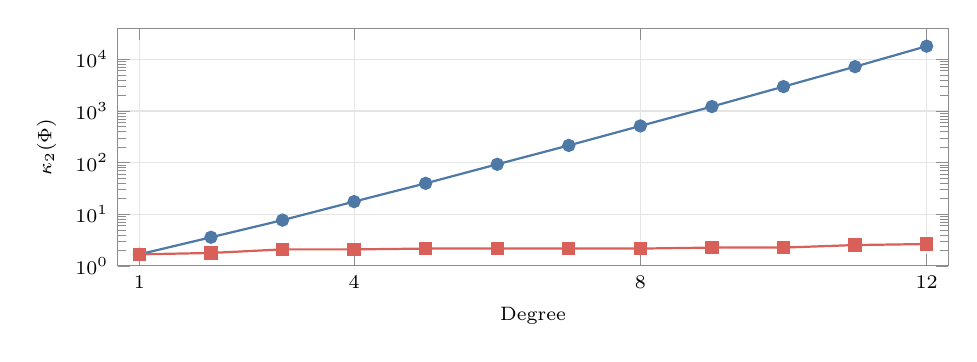
\begin{tikzpicture}
\begin{axis}[width=\linewidth,height=4.6cm,font=\scriptsize,
tick label style={font=\scriptsize},label style={font=\scriptsize},
axis line style={black!45},tick style={black!45},grid=major,grid style={black!10},
scaled ticks=false,xlabel={$x$},ylabel={Response},xmin=-1.05,xmax=1.05,
ymin=-1.6,ymax=1.6,clip=true,unbounded coords=jump,xlabel={Degree},ylabel={$\kappa_2(\Phi)$},xmin=.7,xmax=12.3,ymin=1,ymax=40000,ymode=log,xtick={1,4,8,12},ytick={1,10,100,1000,10000}]
\addplot[blueplot,thick,mark=*] coordinates {(1,1.6752467) (2,3.5809167) (3,7.6956552) (4,17.580814) (5,39.695677) (6,92.797004) (7,215.19859) (8,513.00045) (9,1217.4053) (10,2963.4002) (11,7204.385) (12,17968.471)};
\addplot[redplot,thick,mark=square*] coordinates {(1,1.6752467) (2,1.7798404) (3,2.0875052) (4,2.0891163) (5,2.1630775) (6,2.1631821) (7,2.1641834) (8,2.1649776) (9,2.2614151) (10,2.2629706) (11,2.5336184) (12,2.6516581)};
\end{axis}
\end{tikzpicture}
\end{column}
\begin{column}{.43\textwidth}
\textcolor{blueplot}{\textbf{Monomials}}\par
\small $1,x,x^2,\ldots,x^q$\par\medskip
\textcolor{redplot}{\textbf{Chebyshev basis}}\par
\small $T_0(x),T_1(x),\ldots,T_q(x)$\par\bigskip
\large At degree 12:\par\medskip
\small $\kappa_2:\quad 18{,}000\ \longrightarrow\ 2.65$\par\bigskip
Scale the input; solve with QR or SVD.
\end{column}
\end{columns}
\vfill
\begin{takeaway}A basis change preserves the OLS model space, but generally changes an isotropic ridge penalty.\end{takeaway}
\note{Suggested time: 3 minutes. The figure computes the 2-norm condition number of the full design, including the constant, at 30 equally spaced inputs on [-1,1]. Degree 12 gives 17968.47 for monomials and 2.65166 for the Chebyshev basis. The basis polynomials satisfy T0=1, T1=x, and Tj=2x T(j-1)-T(j-2). Both full-rank designs span exactly the same degree-at-most-q functions; in exact arithmetic their unregularized least-squares fitted values agree. Better coordinates improve numerical computation, but do not remove statistical uncertainty or justify more degrees. Scale raw input ranges before generating high powers; fit any data-dependent preprocessing on training data only. A general non-orthogonal coordinate change does not preserve the Euclidean norm of coefficients. Therefore equal numeric ridge penalties in monomial and Chebyshev coordinates impose different priors on functions; the displayed comparison concerns OLS conditioning only. Polynomial features in d variables through degree q have binomial(d+q,q) distinct terms, including the constant, so feature counts also grow quickly.}
\end{frame}

% Slide 64 | features-4
\begin{frame}{A dot product can hide six features}
\lead{Two-dimensional inputs: $x=(x_1,x_2)$ and $z=(z_1,z_2)$.}
\begin{overlayarea}{\textwidth}{4.45cm}
\only<1>{\vspace{.7cm}\centering
\Large $k(x,z)=(1+x^{\mathsf T}z)^2$\par\bigskip
\large Can this be a dot product in another space?}
\only<2->{
\begin{definitionbox}\[
\phi(x)=\bigl[1,\sqrt{2}x_1,\sqrt{2}x_2,x_1^2,\sqrt{2}x_1x_2,x_2^2\bigr]^{\mathsf T}
\]\end{definitionbox}
\vspace{.15cm}\centering
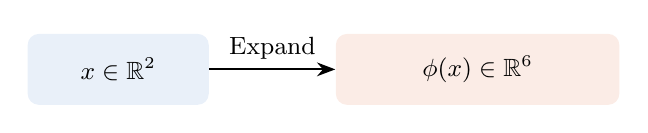
\begin{tikzpicture}[every node/.style={font=\small,align=center}]
\node[fill=definitionblue,rounded corners,minimum width=2.3cm,minimum height=.9cm] (x) {$x\in\R^2$};
\node[fill=takeawaypeach,rounded corners,minimum width=3.6cm,minimum height=.9cm,right=1.6cm of x] (p) {$\phi(x)\in\R^6$};
\draw[-{Stealth},thick] (x)--node[above] {Expand}(p);
\end{tikzpicture}\par\medskip
\uncover<3->{\begin{definitionbox}\[
\phi(x)^{\mathsf T}\phi(z)
=1+2x^{\mathsf T}z+(x^{\mathsf T}z)^2
=(1+x^{\mathsf T}z)^2.
\]\end{definitionbox}}
}
\end{overlayarea}
\end{frame}

% Slide 65 | features-5
\begin{frame}{Compare points without listing features}
\lead{The kernel trick: compute $k(x,z)=\langle\phi(x),\phi(z)\rangle$ directly.}
\vspace{.15cm}\centering
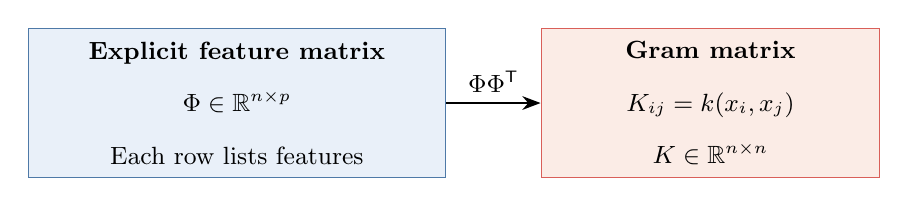
\begin{tikzpicture}[every node/.style={font=\small,align=center}]
\node[fill=definitionblue,draw=blueplot,minimum width=5.3cm,minimum height=1.9cm] (p)
{\textbf{Explicit feature matrix}\\[8pt]$\Phi\in\R^{n\times p}$\\[8pt]Each row lists features};
\node[fill=takeawaypeach,draw=redplot,minimum width=4.3cm,minimum height=1.9cm,right=1.2cm of p] (k)
{\textbf{Gram matrix}\\[8pt]$K_{ij}=k(x_i,x_j)$\\[8pt]$K\in\R^{n\times n}$};
\draw[-{Stealth},thick] (p)--node[above] {$\Phi\Phi^{\mathsf T}$} (k);
\end{tikzpicture}
\vspace{.30cm}
\begin{columns}[t,onlytextwidth]
\begin{column}{.48\textwidth}\small
\textbf{100 inputs, degree at most 3}\par\medskip
$p=\binom{103}{3}=176{,}851$ distinct terms.
\end{column}
\begin{column}{.48\textwidth}\small
\textbf{But the sample size still matters}\par\medskip
Dense $K$: $O(n^2)$ storage; direct solve: $O(n^3)$.
\end{column}
\end{columns}
\end{frame}


\begin{frame}{How to solve the kernelized linear regression?}
	\begin{definitionbox}
	\[  \min_{\theta} J(\theta) = \frac{1}{2n}\sum_{i=1}^n (\phi_i^{\top}\theta - y)^2 + \frac{1}{2} \cdot \lambda \|\theta\|_2  \]
\end{definitionbox}
	\pause
		\begin{definitionbox}
	\[ \theta^* =  (  \Phi^{\top}\Phi + \lambda I  )^{-1} \Phi^{\top} y \]
\end{definitionbox}
	
	\pause
	\vspace{0.1cm}
	$\phi_i$ can have a high dimension $d$. (what is the size of $\Phi^{\top}\Phi$?)
	
	\pause
	\begin{definitionbox}
	\[	\theta^* =  (  \Phi^{\top}\Phi + \lambda I_d )^{-1} \Phi^{\top} y  = \Phi^{\top} (\Phi \Phi^{\top} + \lambda I_n)y = \Phi^{\top} (K+ \lambda I_n)y    \]
	\end{definitionbox}
	

	
\end{frame}
\begin{frame}{How to solve the kernelized linear regression?}

	For new $x$, predict 
\begin{definitionbox}
	\[	\phi(x)^{\top}\theta^*  =\phi)(x)^{\top} \Phi^{\top} (K+ \lambda I_n)y  = v^{\top} (K+ \lambda I_n)y  \],
\end{definitionbox}
where $v^{\top} = [K(x,x_1), K(x,x_2),\ldots, K(x,x_n)  ].$

\end{frame}

% Slide 70 | features-10
\begin{frame}{How local is an RBF similarity?}
\lead{Compare each input to $x=0$. Before fitting any regression coefficients.}
\begin{columns}[c,onlytextwidth]
\begin{column}{.54\textwidth}% Native PGFPlots; generated numeric teaching data.
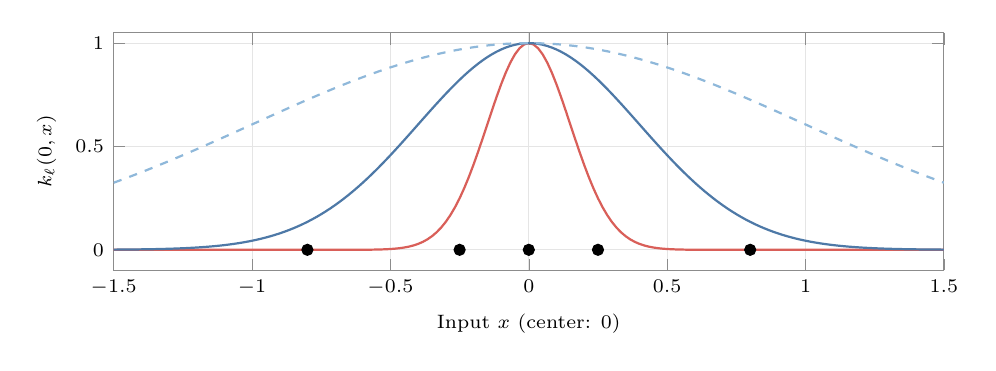
\begin{tikzpicture}
\begin{axis}[width=\linewidth,height=4.6cm,font=\scriptsize,
tick label style={font=\scriptsize},label style={font=\scriptsize},
axis line style={black!45},tick style={black!45},grid=major,grid style={black!10},
scaled ticks=false,xlabel={$x$},ylabel={Response},xmin=-1.05,xmax=1.05,
ymin=-1.6,ymax=1.6,clip=true,unbounded coords=jump,xmin=-1.5,xmax=1.5,ymin=-.1,ymax=1.05,xlabel={Input $x$ (center: 0)},ylabel={$k_\ell(0,x)$},ytick={0,.5,1}]
\addplot[only marks,mark=*,mark size=2pt,black] coordinates {(-0.8,0) (-0.25,0) (0,0) (0.25,0) (0.8,0)};
\only<3->{\addplot[redplot,thick] coordinates {(-1.5,1.9287498e-22) (-1.4833333,5.8229693e-22) (-1.4666667,1.7364066e-21) (-1.45,5.1144237e-21) (-1.4333333,1.4879225e-20) (-1.4166667,4.2756512e-20) (-1.4,1.2135637e-19) (-1.3833333,3.4022106e-19) (-1.3666667,9.4210253e-19) (-1.35,2.5767571e-18) (-1.3333333,6.9612485e-18) (-1.3166667,1.8575441e-17) (-1.3,4.8958653e-17) (-1.2833333,1.2745537e-16) (-1.2666667,3.2773675e-16) (-1.25,8.3239697e-16) (-1.2333333,2.08821e-15) (-1.2166667,5.1743549e-15) (-1.2,1.2664166e-14) (-1.1833333,3.0615072e-14) (-1.1666667,7.3102518e-14) (-1.15,1.7241209e-13) (-1.1333333,4.0164416e-13) (-1.1166667,9.2417353e-13) (-1.1,2.1004093e-12) (-1.0833333,4.7151192e-12) (-1.0666667,1.0454897e-11) (-1.05,2.2897348e-11) (-1.0333333,4.9532353e-11) (-1.0166667,1.0583543e-10) (-1,2.2336314e-10) (-0.98333333,4.6561858e-10) (-0.96666667,9.5871037e-10) (-0.95,1.9497678e-09) (-0.93333333,3.9166674e-09) (-0.91666667,7.7712135e-09) (-0.9,1.522998e-08) (-0.88333333,2.9481403e-08) (-0.86666667,5.6368349e-08) (-0.85,1.0645371e-07) (-0.83333333,1.9857504e-07) (-0.81666667,3.6587004e-07) (-0.8,6.6583615e-07) (-0.78333333,1.1968679e-06) (-0.76666667,2.125022e-06) (-0.75,3.7266532e-06) (-0.73333333,6.4552469e-06) (-0.71666667,1.1044475e-05) (-0.7,1.8664469e-05) (-0.68333333,3.115477e-05) (-0.66666667,5.1365531e-05) (-0.65,8.3648347e-05) (-0.63333333,0.00013454925) (-0.61666667,0.00021376842) (-0.6,0.00033546263) (-0.58333333,0.00051997574) (-0.56666667,0.00079608669) (-0.55,0.00120386) (-0.53333333,0.0017981667) (-0.51666667,0.0026529083) (-0.5,0.0038659201) (-0.48333333,0.005564445) (-0.46666667,0.0079109597) (-0.45,0.011108997) (-0.43333333,0.015408446) (-0.41666667,0.021109656) (-0.4,0.028565501) (-0.38333333,0.038180434) (-0.36666667,0.050405533) (-0.35,0.065728529) (-0.33333333,0.084657989) (-0.31666667,0.10770115) (-0.3,0.13533528) (-0.28333333,0.16797324) (-0.26666667,0.20592425) (-0.25,0.24935221) (-0.23333333,0.2982341) (-0.21666667,0.35232195) (-0.2,0.41111229) (-0.18333333,0.47382673) (-0.16666667,0.53940751) (-0.15,0.60653066) (-0.13333333,0.67363846) (-0.11666667,0.7389913) (-0.1,0.8007374) (-0.083333333,0.85699689) (-0.066666667,0.90595519) (-0.05,0.94595947) (-0.033333333,0.97561098) (-0.016666667,0.99384617) (0,1) (0.016666667,0.99384617) (0.033333333,0.97561098) (0.05,0.94595947) (0.066666667,0.90595519) (0.083333333,0.85699689) (0.1,0.8007374) (0.11666667,0.7389913) (0.13333333,0.67363846) (0.15,0.60653066) (0.16666667,0.53940751) (0.18333333,0.47382673) (0.2,0.41111229) (0.21666667,0.35232195) (0.23333333,0.2982341) (0.25,0.24935221) (0.26666667,0.20592425) (0.28333333,0.16797324) (0.3,0.13533528) (0.31666667,0.10770115) (0.33333333,0.084657989) (0.35,0.065728529) (0.36666667,0.050405533) (0.38333333,0.038180434) (0.4,0.028565501) (0.41666667,0.021109656) (0.43333333,0.015408446) (0.45,0.011108997) (0.46666667,0.0079109597) (0.48333333,0.005564445) (0.5,0.0038659201) (0.51666667,0.0026529083) (0.53333333,0.0017981667) (0.55,0.00120386) (0.56666667,0.00079608669) (0.58333333,0.00051997574) (0.6,0.00033546263) (0.61666667,0.00021376842) (0.63333333,0.00013454925) (0.65,8.3648347e-05) (0.66666667,5.1365531e-05) (0.68333333,3.115477e-05) (0.7,1.8664469e-05) (0.71666667,1.1044475e-05) (0.73333333,6.4552469e-06) (0.75,3.7266532e-06) (0.76666667,2.125022e-06) (0.78333333,1.1968679e-06) (0.8,6.6583615e-07) (0.81666667,3.6587004e-07) (0.83333333,1.9857504e-07) (0.85,1.0645371e-07) (0.86666667,5.6368349e-08) (0.88333333,2.9481403e-08) (0.9,1.522998e-08) (0.91666667,7.7712135e-09) (0.93333333,3.9166674e-09) (0.95,1.9497678e-09) (0.96666667,9.5871037e-10) (0.98333333,4.6561858e-10) (1,2.2336314e-10) (1.0166667,1.0583543e-10) (1.0333333,4.9532353e-11) (1.05,2.2897348e-11) (1.0666667,1.0454897e-11) (1.0833333,4.7151192e-12) (1.1,2.1004093e-12) (1.1166667,9.2417353e-13) (1.1333333,4.0164416e-13) (1.15,1.7241209e-13) (1.1666667,7.3102518e-14) (1.1833333,3.0615072e-14) (1.2,1.2664166e-14) (1.2166667,5.1743549e-15) (1.2333333,2.08821e-15) (1.25,8.3239697e-16) (1.2666667,3.2773675e-16) (1.2833333,1.2745537e-16) (1.3,4.8958653e-17) (1.3166667,1.8575441e-17) (1.3333333,6.9612485e-18) (1.35,2.5767571e-18) (1.3666667,9.4210253e-19) (1.3833333,3.4022106e-19) (1.4,1.2135637e-19) (1.4166667,4.2756512e-20) (1.4333333,1.4879225e-20) (1.45,5.1144237e-21) (1.4666667,1.7364066e-21) (1.4833333,5.8229693e-22) (1.5,1.9287498e-22)};
}
\only<3->{\addplot[blueplot,thick] coordinates {(-1.5,0.00088382631) (-1.4833333,0.0010324011) (-1.4666667,0.00120386) (-1.45,0.0014013594) (-1.4333333,0.00162843) (-1.4166667,0.0018890119) (-1.4,0.0021874911) (-1.3833333,0.0025287385) (-1.3666667,0.0029181496) (-1.35,0.0033616865) (-1.3333333,0.0038659201) (-1.3166667,0.0044380743) (-1.3,0.0050860692) (-1.2833333,0.0058185663) (-1.2666667,0.0066450113) (-1.25,0.0075756774) (-1.2333333,0.0086217067) (-1.2166667,0.0097951486) (-1.2,0.011108997) (-1.1833333,0.01257722) (-1.1666667,0.014214791) (-1.15,0.016037709) (-1.1333333,0.018063013) (-1.1166667,0.020308792) (-1.1,0.022794181) (-1.0833333,0.025539354) (-1.0666667,0.028565501) (-1.05,0.031894793) (-1.0333333,0.03555034) (-1.0166667,0.039556125) (-1,0.043936934) (-0.98333333,0.048718259) (-0.96666667,0.053926197) (-0.95,0.059587319) (-0.93333333,0.065728529) (-0.91666667,0.072376903) (-0.9,0.079559509) (-0.88333333,0.087303209) (-0.86666667,0.095634445) (-0.85,0.104579) (-0.83333333,0.11416176) (-0.81666667,0.12440643) (-0.8,0.13533528) (-0.78333333,0.14696883) (-0.76666667,0.15932557) (-0.75,0.17242162) (-0.73333333,0.18627046) (-0.71666667,0.20088258) (-0.7,0.21626517) (-0.68333333,0.23242182) (-0.66666667,0.24935221) (-0.65,0.26705184) (-0.63333333,0.28551171) (-0.61666667,0.30471814) (-0.6,0.32465247) (-0.58333333,0.34529089) (-0.56666667,0.3666043) (-0.55,0.38855813) (-0.53333333,0.41111229) (-0.51666667,0.43422112) (-0.5,0.45783336) (-0.48333333,0.48189226) (-0.46666667,0.50633562) (-0.45,0.53109599) (-0.43333333,0.55610088) (-0.41666667,0.58127302) (-0.4,0.60653066) (-0.38333333,0.631788) (-0.36666667,0.65695557) (-0.35,0.68194075) (-0.33333333,0.70664828) (-0.31666667,0.73098082) (-0.3,0.7548396) (-0.28333333,0.77812503) (-0.26666667,0.8007374) (-0.25,0.82257756) (-0.23333333,0.84354765) (-0.21666667,0.86355181) (-0.2,0.8824969) (-0.18333333,0.90029326) (-0.16666667,0.91685536) (-0.15,0.93210249) (-0.13333333,0.94595947) (-0.11666667,0.95835719) (-0.1,0.96923323) (-0.083333333,0.97853239) (-0.066666667,0.98620712) (-0.05,0.99221794) (-0.033333333,0.9965338) (-0.016666667,0.99913232) (0,1) (0.016666667,0.99913232) (0.033333333,0.9965338) (0.05,0.99221794) (0.066666667,0.98620712) (0.083333333,0.97853239) (0.1,0.96923323) (0.11666667,0.95835719) (0.13333333,0.94595947) (0.15,0.93210249) (0.16666667,0.91685536) (0.18333333,0.90029326) (0.2,0.8824969) (0.21666667,0.86355181) (0.23333333,0.84354765) (0.25,0.82257756) (0.26666667,0.8007374) (0.28333333,0.77812503) (0.3,0.7548396) (0.31666667,0.73098082) (0.33333333,0.70664828) (0.35,0.68194075) (0.36666667,0.65695557) (0.38333333,0.631788) (0.4,0.60653066) (0.41666667,0.58127302) (0.43333333,0.55610088) (0.45,0.53109599) (0.46666667,0.50633562) (0.48333333,0.48189226) (0.5,0.45783336) (0.51666667,0.43422112) (0.53333333,0.41111229) (0.55,0.38855813) (0.56666667,0.3666043) (0.58333333,0.34529089) (0.6,0.32465247) (0.61666667,0.30471814) (0.63333333,0.28551171) (0.65,0.26705184) (0.66666667,0.24935221) (0.68333333,0.23242182) (0.7,0.21626517) (0.71666667,0.20088258) (0.73333333,0.18627046) (0.75,0.17242162) (0.76666667,0.15932557) (0.78333333,0.14696883) (0.8,0.13533528) (0.81666667,0.12440643) (0.83333333,0.11416176) (0.85,0.104579) (0.86666667,0.095634445) (0.88333333,0.087303209) (0.9,0.079559509) (0.91666667,0.072376903) (0.93333333,0.065728529) (0.95,0.059587319) (0.96666667,0.053926197) (0.98333333,0.048718259) (1,0.043936934) (1.0166667,0.039556125) (1.0333333,0.03555034) (1.05,0.031894793) (1.0666667,0.028565501) (1.0833333,0.025539354) (1.1,0.022794181) (1.1166667,0.020308792) (1.1333333,0.018063013) (1.15,0.016037709) (1.1666667,0.014214791) (1.1833333,0.01257722) (1.2,0.011108997) (1.2166667,0.0097951486) (1.2333333,0.0086217067) (1.25,0.0075756774) (1.2666667,0.0066450113) (1.2833333,0.0058185663) (1.3,0.0050860692) (1.3166667,0.0044380743) (1.3333333,0.0038659201) (1.35,0.0033616865) (1.3666667,0.0029181496) (1.3833333,0.0025287385) (1.4,0.0021874911) (1.4166667,0.0018890119) (1.4333333,0.00162843) (1.45,0.0014013594) (1.4666667,0.00120386) (1.4833333,0.0010324011) (1.5,0.00088382631)};
}
\only<3->{\addplot[lightplot,thick,dashed] coordinates {(-1.5,0.32465247) (-1.4833333,0.33282485) (-1.4666667,0.3411082) (-1.45,0.3495006) (-1.4333333,0.35800003) (-1.4166667,0.3666043) (-1.4,0.3753111) (-1.3833333,0.38411797) (-1.3666667,0.39302231) (-1.35,0.40202138) (-1.3333333,0.41111229) (-1.3166667,0.42029201) (-1.3,0.42955736) (-1.2833333,0.43890503) (-1.2666667,0.44833156) (-1.25,0.45783336) (-1.2333333,0.46740668) (-1.2166667,0.47704765) (-1.2,0.48675226) (-1.1833333,0.49651634) (-1.1666667,0.50633562) (-1.15,0.51620567) (-1.1333333,0.52612196) (-1.1166667,0.53607981) (-1.1,0.54607443) (-1.0833333,0.55610088) (-1.0666667,0.56615415) (-1.05,0.57622907) (-1.0333333,0.5863204) (-1.0166667,0.59642275) (-1,0.60653066) (-0.98333333,0.61663856) (-0.96666667,0.6267408) (-0.95,0.63683161) (-0.93333333,0.64690518) (-0.91666667,0.65695557) (-0.9,0.66697681) (-0.88333333,0.67696285) (-0.86666667,0.68690756) (-0.85,0.69680478) (-0.83333333,0.70664828) (-0.81666667,0.7164318) (-0.8,0.72614904) (-0.78333333,0.73579366) (-0.76666667,0.7453593) (-0.75,0.7548396) (-0.73333333,0.76422817) (-0.71666667,0.77351861) (-0.7,0.78270454) (-0.68333333,0.79177959) (-0.66666667,0.8007374) (-0.65,0.80957165) (-0.63333333,0.81827603) (-0.61666667,0.82684429) (-0.6,0.83527021) (-0.58333333,0.84354765) (-0.56666667,0.85167051) (-0.55,0.85963276) (-0.53333333,0.86742847) (-0.51666667,0.87505178) (-0.5,0.8824969) (-0.48333333,0.88975818) (-0.46666667,0.89683006) (-0.45,0.90370708) (-0.43333333,0.91038391) (-0.41666667,0.91685536) (-0.4,0.92311635) (-0.38333333,0.92916196) (-0.36666667,0.9349874) (-0.35,0.94058806) (-0.33333333,0.94595947) (-0.31666667,0.95109732) (-0.3,0.95599748) (-0.28333333,0.96065601) (-0.26666667,0.96506912) (-0.25,0.96923323) (-0.23333333,0.97314496) (-0.21666667,0.97680111) (-0.2,0.98019867) (-0.18333333,0.98333487) (-0.16666667,0.98620712) (-0.15,0.98881304) (-0.13333333,0.9911505) (-0.11666667,0.99321755) (-0.1,0.99501248) (-0.083333333,0.9965338) (-0.066666667,0.99778025) (-0.05,0.99875078) (-0.033333333,0.9994446) (-0.016666667,0.99986112) (0,1) (0.016666667,0.99986112) (0.033333333,0.9994446) (0.05,0.99875078) (0.066666667,0.99778025) (0.083333333,0.9965338) (0.1,0.99501248) (0.11666667,0.99321755) (0.13333333,0.9911505) (0.15,0.98881304) (0.16666667,0.98620712) (0.18333333,0.98333487) (0.2,0.98019867) (0.21666667,0.97680111) (0.23333333,0.97314496) (0.25,0.96923323) (0.26666667,0.96506912) (0.28333333,0.96065601) (0.3,0.95599748) (0.31666667,0.95109732) (0.33333333,0.94595947) (0.35,0.94058806) (0.36666667,0.9349874) (0.38333333,0.92916196) (0.4,0.92311635) (0.41666667,0.91685536) (0.43333333,0.91038391) (0.45,0.90370708) (0.46666667,0.89683006) (0.48333333,0.88975818) (0.5,0.8824969) (0.51666667,0.87505178) (0.53333333,0.86742847) (0.55,0.85963276) (0.56666667,0.85167051) (0.58333333,0.84354765) (0.6,0.83527021) (0.61666667,0.82684429) (0.63333333,0.81827603) (0.65,0.80957165) (0.66666667,0.8007374) (0.68333333,0.79177959) (0.7,0.78270454) (0.71666667,0.77351861) (0.73333333,0.76422817) (0.75,0.7548396) (0.76666667,0.7453593) (0.78333333,0.73579366) (0.8,0.72614904) (0.81666667,0.7164318) (0.83333333,0.70664828) (0.85,0.69680478) (0.86666667,0.68690756) (0.88333333,0.67696285) (0.9,0.66697681) (0.91666667,0.65695557) (0.93333333,0.64690518) (0.95,0.63683161) (0.96666667,0.6267408) (0.98333333,0.61663856) (1,0.60653066) (1.0166667,0.59642275) (1.0333333,0.5863204) (1.05,0.57622907) (1.0666667,0.56615415) (1.0833333,0.55610088) (1.1,0.54607443) (1.1166667,0.53607981) (1.1333333,0.52612196) (1.15,0.51620567) (1.1666667,0.50633562) (1.1833333,0.49651634) (1.2,0.48675226) (1.2166667,0.47704765) (1.2333333,0.46740668) (1.25,0.45783336) (1.2666667,0.44833156) (1.2833333,0.43890503) (1.3,0.42955736) (1.3166667,0.42029201) (1.3333333,0.41111229) (1.35,0.40202138) (1.3666667,0.39302231) (1.3833333,0.38411797) (1.4,0.3753111) (1.4166667,0.3666043) (1.4333333,0.35800003) (1.45,0.3495006) (1.4666667,0.3411082) (1.4833333,0.33282485) (1.5,0.32465247)};
}
\end{axis}
\end{tikzpicture}
\end{column}
\begin{column}{.42\textwidth}
\begin{overlayarea}{\linewidth}{4.1cm}
\only<1>{\vspace{.55cm}\large Which point is more similar?\par\bigskip
$x=0.25$\quad or\quad $x=0.8$\par\bigskip
\small What should ``nearby'' mean?}
\only<2>{\vspace{.35cm}\begin{definitionbox}\[
k_\ell(x,z)=e^{-\|x-z\|^2/(2\ell^2)}
\]\end{definitionbox}\par\medskip
\large At distance $\ell$:\par\medskip
$k=e^{-1/2}\approx0.607$\par\medskip
\small Predict the effect of increasing $\ell$.}
\only<3>{\vspace{.35cm}
\textcolor{redplot}{\textbf{$\ell=0.15$: narrow}}\par\medskip
\textcolor{blueplot}{\textbf{$\ell=0.40$: intermediate}}\par\medskip
\textcolor{lightplot}{\textbf{$\ell=1.00$: broad}}\par\medskip
\large Scale inputs before measuring distance.}
\end{overlayarea}
\end{column}
\end{columns}
\vfill
\uncover<3->{\begin{takeaway}The bandwidth sets similarity range; learned coefficients set the prediction.\end{takeaway}}
\note{Suggested time: 4 minutes. Build 1: show only five input locations and ask which of 0.25 and 0.8 should be more similar to zero; wait 10 seconds. Build 2: reveal the RBF definition and its interpretable distance scale. Ask what happens when ell increases, then pause for a prediction. Build 3: reveal the three curves. At fixed nonzero distance, increasing ell increases similarity, broadening the neighborhood. The horizontal positions of points are their signed offsets from the fixed center zero; vertical zero is just a marker baseline, not a target value. The graph is a kernel section, not a fitted response curve. In kernel ridge, coefficients may be positive or negative, so similarity is not itself the final influence or prediction. For multiple input coordinates, scales determine distances; train-only standardization and a validated bandwidth are part of the model. The RBF has an infinite-dimensional feature representation, but KRR still solves the finite system from the previous slides.}
\end{frame}

% Slide 71 | features-11
\begin{frame}{Bandwidth and penalty do different jobs}
\lead{Same observations. Centered RBF kernel ridge with an unpenalized intercept.}
\begin{columns}[t,onlytextwidth]
\begin{column}{.49\textwidth}\centering
\small\textbf{Change $\ell$; fix $\lambda=0.001$}\par
% Native PGFPlots; generated numeric teaching data.
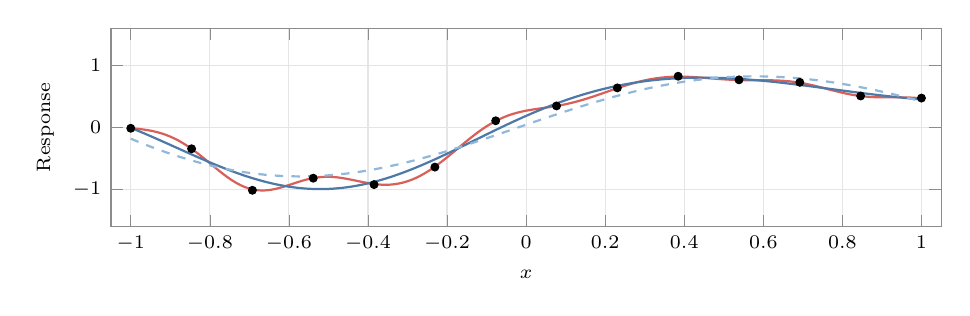
\begin{tikzpicture}
\begin{axis}[width=\linewidth,height=4.6cm,font=\scriptsize,
tick label style={font=\scriptsize},label style={font=\scriptsize},
axis line style={black!45},tick style={black!45},grid=major,grid style={black!10},
scaled ticks=false,xlabel={$x$},ylabel={Response},xmin=-1.05,xmax=1.05,
ymin=-1.6,ymax=1.6,clip=true,unbounded coords=jump,height=4.1cm]
\addplot[redplot,thick] coordinates {(-1,-0.013641226) (-0.98888889,-0.019320907) (-0.97777778,-0.026423231) (-0.96666667,-0.035326644) (-0.95555556,-0.046436246) (-0.94444444,-0.060170796) (-0.93333333,-0.07694672) (-0.92222222,-0.09715952) (-0.91111111,-0.1211632) (-0.9,-0.14924847) (-0.88888889,-0.18162088) (-0.87777778,-0.21837982) (-0.86666667,-0.2594999) (-0.85555556,-0.30481586) (-0.84444444,-0.3540123) (-0.83333333,-0.40661935) (-0.82222222,-0.46201513) (-0.81111111,-0.51943564) (-0.8,-0.57799215) (-0.78888889,-0.6366959) (-0.77777778,-0.69448941) (-0.76666667,-0.75028318) (-0.75555556,-0.80299622) (-0.74444444,-0.8515986) (-0.73333333,-0.89515364) (-0.72222222,-0.93285792) (-0.71111111,-0.96407644) (-0.7,-0.98837141) (-0.68888889,-1.0055226) (-0.67777778,-1.0155384) (-0.66666667,-1.0186564) (-0.65555556,-1.0153338) (-0.64444444,-1.0062282) (-0.63333333,-0.99216878) (-0.62222222,-0.97412087) (-0.61111111,-0.95314452) (-0.6,-0.9303498) (-0.58888889,-0.90685099) (-0.57777778,-0.8837218) (-0.56666667,-0.86195394) (-0.55555556,-0.84242061) (-0.54444444,-0.82584671) (-0.53333333,-0.81278659) (-0.52222222,-0.80361019) (-0.51111111,-0.79849761) (-0.5,-0.79744183) (-0.48888889,-0.80025905) (-0.47777778,-0.80660536) (-0.46666667,-0.81599881) (-0.45555556,-0.82784509) (-0.44444444,-0.84146551) (-0.43333333,-0.85612567) (-0.42222222,-0.87106347) (-0.41111111,-0.88551514) (-0.4,-0.89873841) (-0.38888889,-0.91003215) (-0.37777778,-0.91875198) (-0.36666667,-0.92432199) (-0.35555556,-0.92624266) (-0.34444444,-0.92409553) (-0.33333333,-0.9175452) (-0.32222222,-0.90633952) (-0.31111111,-0.89030856) (-0.3,-0.8693631) (-0.28888889,-0.84349314) (-0.27777778,-0.81276679) (-0.26666667,-0.7773295) (-0.25555556,-0.73740365) (-0.24444444,-0.69328799) (-0.23333333,-0.64535653) (-0.22222222,-0.59405621) (-0.21111111,-0.53990281) (-0.2,-0.48347448) (-0.18888889,-0.42540254) (-0.17777778,-0.36635937) (-0.16666667,-0.3070435) (-0.15555556,-0.24816208) (-0.14444444,-0.1904116) (-0.13333333,-0.13445732) (-0.12222222,-0.080912706) (-0.11111111,-0.030319757) (-0.1,0.016868688) (-0.088888889,0.060303613) (-0.077777778,0.099750644) (-0.066666667,0.13509639) (-0.055555556,0.16634991) (-0.044444444,0.19363925) (-0.033333333,0.21720319) (-0.022222222,0.23737862) (-0.011111111,0.25458438) (0,0.26930222) (0.011111111,0.28205596) (0.022222222,0.29338992) (0.033333333,0.30384751) (0.044444444,0.31395112) (0.055555556,0.32418395) (0.066666667,0.33497472) (0.077777778,0.3466855) (0.088888889,0.35960322) (0.1,0.3739348) (0.11111111,0.3898059) (0.12222222,0.40726297) (0.13333333,0.42627832) (0.14444444,0.44675749) (0.15555556,0.46854841) (0.16666667,0.49145179) (0.17777778,0.51523196) (0.18888889,0.5396276) (0.2,0.56436199) (0.21111111,0.58915214) (0.22222222,0.61371682) (0.23333333,0.6377831) (0.24444444,0.6610916) (0.25555556,0.68340049) (0.26666667,0.70448844) (0.27777778,0.72415686) (0.28888889,0.74223164) (0.3,0.75856471) (0.31111111,0.77303568) (0.32222222,0.78555349) (0.33333333,0.7960584) (0.34444444,0.80452394) (0.35555556,0.81095888) (0.36666667,0.81540875) (0.37777778,0.81795687) (0.38888889,0.81872429) (0.4,0.81786857) (0.41111111,0.8155811) (0.42222222,0.81208273) (0.43333333,0.80761792) (0.44444444,0.80244717) (0.45555556,0.79683828) (0.46666667,0.79105651) (0.47777778,0.78535422) (0.48888889,0.77996036) (0.5,0.77507043) (0.51111111,0.77083732) (0.52222222,0.76736366) (0.53333333,0.76469613) (0.54444444,0.76282192) (0.55555556,0.76166801) (0.56666667,0.76110303) (0.57777778,0.76094212) (0.58888889,0.76095445) (0.6,0.76087333) (0.61111111,0.7604085) (0.62222222,0.7592601) (0.63333333,0.75713371) (0.64444444,0.75375582) (0.65555556,0.74888882) (0.66666667,0.74234487) (0.67777778,0.73399777) (0.68888889,0.72379219) (0.7,0.71174963) (0.71111111,0.69797068) (0.72222222,0.6826333) (0.73333333,0.66598723) (0.74444444,0.64834442) (0.75555556,0.63006624) (0.76666667,0.61154779) (0.77777778,0.59320018) (0.78888889,0.57543169) (0.8,0.55862874) (0.81111111,0.54313754) (0.82222222,0.52924762) (0.83333333,0.51717778) (0.84444444,0.50706535) (0.85555556,0.49895933) (0.86666667,0.49281761) (0.87777778,0.48850853) (0.88888889,0.48581665) (0.9,0.48445242) (0.91111111,0.48406531) (0.92222222,0.48425964) (0.93333333,0.48461244) (0.94444444,0.48469233) (0.95555556,0.48407856) (0.96666667,0.48237928) (0.97777778,0.47924804) (0.98888889,0.47439795) (1,0.46761266)};
\addplot[blueplot,thick] coordinates {(-1,-0.007421128) (-0.98888889,-0.036281375) (-0.97777778,-0.065700616) (-0.96666667,-0.095627054) (-0.95555556,-0.12600654) (-0.94444444,-0.15678271) (-0.93333333,-0.18789716) (-0.92222222,-0.21928959) (-0.91111111,-0.250898) (-0.9,-0.28265884) (-0.88888889,-0.3145072) (-0.87777778,-0.34637703) (-0.86666667,-0.37820131) (-0.85555556,-0.40991224) (-0.84444444,-0.44144147) (-0.83333333,-0.47272026) (-0.82222222,-0.50367975) (-0.81111111,-0.53425109) (-0.8,-0.56436572) (-0.78888889,-0.5939555) (-0.77777778,-0.62295298) (-0.76666667,-0.65129155) (-0.75555556,-0.67890565) (-0.74444444,-0.70573099) (-0.73333333,-0.7317047) (-0.72222222,-0.75676553) (-0.71111111,-0.78085402) (-0.7,-0.80391271) (-0.68888889,-0.82588624) (-0.67777778,-0.84672157) (-0.66666667,-0.86636809) (-0.65555556,-0.88477779) (-0.64444444,-0.90190538) (-0.63333333,-0.91770845) (-0.62222222,-0.93214752) (-0.61111111,-0.94518624) (-0.6,-0.95679141) (-0.58888889,-0.96693315) (-0.57777778,-0.97558491) (-0.56666667,-0.9827236) (-0.55555556,-0.98832962) (-0.54444444,-0.99238693) (-0.53333333,-0.99488309) (-0.52222222,-0.99580929) (-0.51111111,-0.99516039) (-0.5,-0.9929349) (-0.48888889,-0.98913502) (-0.47777778,-0.98376661) (-0.46666667,-0.97683916) (-0.45555556,-0.96836578) (-0.44444444,-0.95836318) (-0.43333333,-0.94685155) (-0.42222222,-0.93385457) (-0.41111111,-0.9193993) (-0.4,-0.90351609) (-0.38888889,-0.88623851) (-0.37777778,-0.86760322) (-0.36666667,-0.84764989) (-0.35555556,-0.82642103) (-0.34444444,-0.8039619) (-0.33333333,-0.78032032) (-0.32222222,-0.75554655) (-0.31111111,-0.72969315) (-0.3,-0.70281474) (-0.28888889,-0.6749679) (-0.27777778,-0.64621093) (-0.26666667,-0.61660371) (-0.25555556,-0.58620746) (-0.24444444,-0.55508458) (-0.23333333,-0.52329843) (-0.22222222,-0.49091313) (-0.21111111,-0.45799337) (-0.2,-0.42460416) (-0.18888889,-0.39081068) (-0.17777778,-0.35667803) (-0.16666667,-0.32227105) (-0.15555556,-0.28765413) (-0.14444444,-0.25289099) (-0.13333333,-0.21804451) (-0.12222222,-0.18317654) (-0.11111111,-0.1483477) (-0.1,-0.11361728) (-0.088888889,-0.079043001) (-0.077777778,-0.044680917) (-0.066666667,-0.010585257) (-0.055555556,0.023191698) (-0.044444444,0.056599731) (-0.033333333,0.089590797) (-0.022222222,0.12211911) (-0.011111111,0.15414121) (0,0.18561607) (0.011111111,0.2165051) (0.022222222,0.24677219) (0.033333333,0.27638379) (0.044444444,0.30530884) (0.055555556,0.33351885) (0.066666667,0.36098783) (0.077777778,0.38769231) (0.088888889,0.41361125) (0.1,0.43872607) (0.11111111,0.46302053) (0.12222222,0.48648067) (0.13333333,0.50909481) (0.14444444,0.53085337) (0.15555556,0.55174886) (0.16666667,0.57177575) (0.17777778,0.59093039) (0.18888889,0.6092109) (0.2,0.62661709) (0.21111111,0.64315033) (0.22222222,0.65881349) (0.23333333,0.67361078) (0.24444444,0.68754769) (0.25555556,0.70063089) (0.26666667,0.71286813) (0.27777778,0.72426812) (0.28888889,0.7348405) (0.3,0.74459571) (0.31111111,0.75354495) (0.32222222,0.76170006) (0.33333333,0.76907352) (0.34444444,0.77567834) (0.35555556,0.78152804) (0.36666667,0.78663658) (0.37777778,0.79101835) (0.38888889,0.79468811) (0.4,0.79766099) (0.41111111,0.79995245) (0.42222222,0.80157829) (0.43333333,0.80255459) (0.44444444,0.80289777) (0.45555556,0.80262455) (0.46666667,0.80175195) (0.47777778,0.80029731) (0.48888889,0.79827829) (0.5,0.79571288) (0.51111111,0.7926194) (0.52222222,0.78901654) (0.53333333,0.7849233) (0.54444444,0.78035907) (0.55555556,0.77534361) (0.56666667,0.76989704) (0.57777778,0.76403983) (0.58888889,0.75779282) (0.6,0.75117723) (0.61111111,0.74421458) (0.62222222,0.73692674) (0.63333333,0.72933587) (0.64444444,0.72146441) (0.65555556,0.71333505) (0.66666667,0.70497067) (0.67777778,0.69639432) (0.68888889,0.68762918) (0.7,0.67869848) (0.71111111,0.66962546) (0.72222222,0.66043332) (0.73333333,0.65114516) (0.74444444,0.64178387) (0.75555556,0.63237211) (0.76666667,0.62293223) (0.77777778,0.61348617) (0.78888889,0.60405543) (0.8,0.59466094) (0.81111111,0.58532305) (0.82222222,0.57606142) (0.83333333,0.56689494) (0.84444444,0.5578417) (0.85555556,0.5489189) (0.86666667,0.54014277) (0.87777778,0.53152856) (0.88888889,0.52309045) (0.9,0.51484152) (0.91111111,0.5067937) (0.92222222,0.49895774) (0.93333333,0.49134316) (0.94444444,0.48395825) (0.95555556,0.47681007) (0.96666667,0.46990438) (0.97777778,0.46324571) (0.98888889,0.45683729) (1,0.45068113)};
\addplot[lightplot,thick,dashed] coordinates {(-1,-0.18309646) (-0.98888889,-0.21246803) (-0.97777778,-0.24127209) (-0.96666667,-0.26949138) (-0.95555556,-0.29710904) (-0.94444444,-0.3241086) (-0.93333333,-0.35047404) (-0.92222222,-0.37618979) (-0.91111111,-0.40124072) (-0.9,-0.42561218) (-0.88888889,-0.44929002) (-0.87777778,-0.47226058) (-0.86666667,-0.49451072) (-0.85555556,-0.51602783) (-0.84444444,-0.53679986) (-0.83333333,-0.55681529) (-0.82222222,-0.57606318) (-0.81111111,-0.59453318) (-0.8,-0.6122155) (-0.78888889,-0.62910098) (-0.77777778,-0.64518106) (-0.76666667,-0.6604478) (-0.75555556,-0.67489388) (-0.74444444,-0.68851263) (-0.73333333,-0.70129802) (-0.72222222,-0.71324466) (-0.71111111,-0.72434784) (-0.7,-0.7346035) (-0.68888889,-0.74400824) (-0.67777778,-0.75255934) (-0.66666667,-0.76025477) (-0.65555556,-0.76709315) (-0.64444444,-0.77307382) (-0.63333333,-0.77819676) (-0.62222222,-0.78246268) (-0.61111111,-0.78587294) (-0.6,-0.7884296) (-0.58888889,-0.79013542) (-0.57777778,-0.7909938) (-0.56666667,-0.79100888) (-0.55555556,-0.79018541) (-0.54444444,-0.78852888) (-0.53333333,-0.78604541) (-0.52222222,-0.78274178) (-0.51111111,-0.77862547) (-0.5,-0.77370457) (-0.48888889,-0.76798783) (-0.47777778,-0.76148466) (-0.46666667,-0.75420507) (-0.45555556,-0.74615971) (-0.44444444,-0.73735983) (-0.43333333,-0.7278173) (-0.42222222,-0.71754456) (-0.41111111,-0.70655464) (-0.4,-0.69486115) (-0.38888889,-0.68247824) (-0.37777778,-0.6694206) (-0.36666667,-0.65570347) (-0.35555556,-0.64134258) (-0.34444444,-0.62635417) (-0.33333333,-0.61075497) (-0.32222222,-0.59456218) (-0.31111111,-0.57779345) (-0.3,-0.56046687) (-0.28888889,-0.54260095) (-0.27777778,-0.52421459) (-0.26666667,-0.50532709) (-0.25555556,-0.48595811) (-0.24444444,-0.46612767) (-0.23333333,-0.44585611) (-0.22222222,-0.42516407) (-0.21111111,-0.4040725) (-0.2,-0.38260262) (-0.18888889,-0.36077588) (-0.17777778,-0.33861398) (-0.16666667,-0.31613882) (-0.15555556,-0.29337252) (-0.14444444,-0.27033732) (-0.13333333,-0.24705564) (-0.12222222,-0.22355003) (-0.11111111,-0.19984312) (-0.1,-0.17595767) (-0.088888889,-0.15191645) (-0.077777778,-0.12774231) (-0.066666667,-0.10345811) (-0.055555556,-0.079086717) (-0.044444444,-0.054650962) (-0.033333333,-0.030173646) (-0.022222222,-0.0056775044) (-0.011111111,0.018814812) (0,0.043280756) (0.011111111,0.067697906) (0.022222222,0.092043987) (0.033333333,0.11629689) (0.044444444,0.14043469) (0.055555556,0.16443566) (0.066666667,0.18827832) (0.077777778,0.21194141) (0.088888889,0.23540394) (0.1,0.25864521) (0.11111111,0.28164482) (0.12222222,0.30438266) (0.13333333,0.32683899) (0.14444444,0.34899441) (0.15555556,0.37082986) (0.16666667,0.39232672) (0.17777778,0.41346672) (0.18888889,0.43423202) (0.2,0.45460523) (0.21111111,0.47456937) (0.22222222,0.49410794) (0.23333333,0.51320491) (0.24444444,0.53184472) (0.25555556,0.55001232) (0.26666667,0.56769317) (0.27777778,0.58487322) (0.28888889,0.60153898) (0.3,0.61767749) (0.31111111,0.63327632) (0.32222222,0.64832361) (0.33333333,0.66280806) (0.34444444,0.67671896) (0.35555556,0.69004614) (0.36666667,0.70278004) (0.37777778,0.7149117) (0.38888889,0.72643271) (0.4,0.73733531) (0.41111111,0.74761231) (0.42222222,0.75725713) (0.43333333,0.7662638) (0.44444444,0.77462697) (0.45555556,0.78234187) (0.46666667,0.78940438) (0.47777778,0.79581095) (0.48888889,0.80155867) (0.5,0.80664523) (0.51111111,0.81106891) (0.52222222,0.81482861) (0.53333333,0.81792383) (0.54444444,0.82035465) (0.55555556,0.82212177) (0.56666667,0.82322645) (0.57777778,0.82367053) (0.58888889,0.82345646) (0.6,0.82258721) (0.61111111,0.82106635) (0.62222222,0.81889799) (0.63333333,0.81608678) (0.64444444,0.81263791) (0.65555556,0.8085571) (0.66666667,0.8038506) (0.67777778,0.79852514) (0.68888889,0.79258797) (0.7,0.78604683) (0.71111111,0.77890991) (0.72222222,0.77118589) (0.73333333,0.76288389) (0.74444444,0.75401348) (0.75555556,0.74458463) (0.76666667,0.73460776) (0.77777778,0.72409367) (0.78888889,0.71305355) (0.8,0.70149895) (0.81111111,0.6894418) (0.82222222,0.67689438) (0.83333333,0.66386926) (0.84444444,0.65037938) (0.85555556,0.63643793) (0.86666667,0.62205841) (0.87777778,0.6072546) (0.88888889,0.5920405) (0.9,0.57643039) (0.91111111,0.56043875) (0.92222222,0.54408026) (0.93333333,0.52736981) (0.94444444,0.51032247) (0.95555556,0.49295346) (0.96666667,0.47527814) (0.97777778,0.45731201) (0.98888889,0.43907067) (1,0.42056985)};
\addplot[only marks,mark=*,mark size=1.4pt,black] coordinates {(-1,-0.014539702) (-0.84615385,-0.34516883) (-0.69230769,-1.0151104) (-0.53846154,-0.82009194) (-0.38461538,-0.92297015) (-0.23076923,-0.64102463) (-0.076923077,0.10647764) (0.076923077,0.3460617) (0.23076923,0.63699851) (0.38461538,0.82531436) (0.53846154,0.76750888) (0.69230769,0.72707693) (0.84615385,0.50661061) (1,0.47271884)};
\end{axis}
\end{tikzpicture}
\par
{\scriptsize\textcolor{redplot}{$\ell=.12$}\quad\textcolor{blueplot}{$\ell=.40$}\quad\textcolor{lightplot}{$\ell=1.00$}}
\end{column}
\begin{column}{.49\textwidth}\centering
\small\textbf{Change $\lambda$; fix $\ell=0.40$}\par
% Native PGFPlots; generated numeric teaching data.
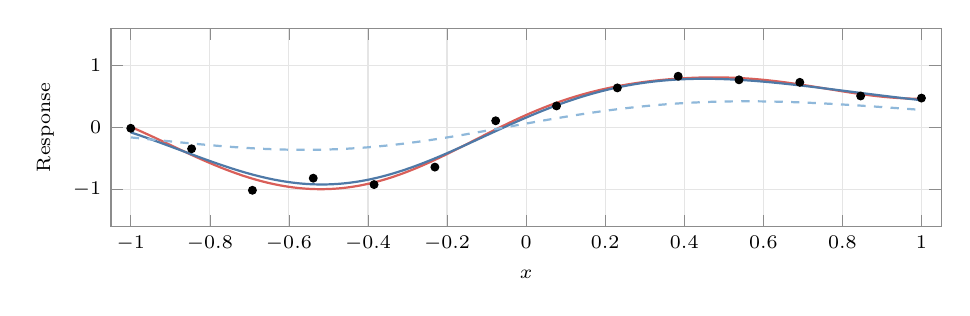
\begin{tikzpicture}
\begin{axis}[width=\linewidth,height=4.6cm,font=\scriptsize,
tick label style={font=\scriptsize},label style={font=\scriptsize},
axis line style={black!45},tick style={black!45},grid=major,grid style={black!10},
scaled ticks=false,xlabel={$x$},ylabel={Response},xmin=-1.05,xmax=1.05,
ymin=-1.6,ymax=1.6,clip=true,unbounded coords=jump,height=4.1cm]
\addplot[redplot,thick] coordinates {(-1,0.0074516944) (-0.98888889,-0.023158298) (-0.97777778,-0.054402483) (-0.96666667,-0.086203042) (-0.95555556,-0.11848042) (-0.94444444,-0.15115371) (-0.93333333,-0.18414108) (-0.92222222,-0.21736013) (-0.91111111,-0.25072833) (-0.9,-0.2841633) (-0.88888889,-0.31758328) (-0.87777778,-0.35090735) (-0.86666667,-0.38405584) (-0.85555556,-0.41695055) (-0.84444444,-0.44951506) (-0.83333333,-0.48167497) (-0.82222222,-0.51335806) (-0.81111111,-0.54449453) (-0.8,-0.57501711) (-0.78888889,-0.60486122) (-0.77777778,-0.63396503) (-0.76666667,-0.66226955) (-0.75555556,-0.68971864) (-0.74444444,-0.71625905) (-0.73333333,-0.74184041) (-0.72222222,-0.76641517) (-0.71111111,-0.78993857) (-0.7,-0.81236857) (-0.68888889,-0.83366577) (-0.67777778,-0.85379332) (-0.66666667,-0.87271679) (-0.65555556,-0.89040411) (-0.64444444,-0.90682544) (-0.63333333,-0.92195307) (-0.62222222,-0.93576132) (-0.61111111,-0.94822645) (-0.6,-0.95932657) (-0.58888889,-0.96904159) (-0.57777778,-0.97735314) (-0.56666667,-0.98424454) (-0.55555556,-0.98970077) (-0.54444444,-0.99370849) (-0.53333333,-0.99625602) (-0.52222222,-0.99733342) (-0.51111111,-0.99693247) (-0.5,-0.99504683) (-0.48888889,-0.99167205) (-0.47777778,-0.98680574) (-0.46666667,-0.98044764) (-0.45555556,-0.97259977) (-0.44444444,-0.96326658) (-0.43333333,-0.95245507) (-0.42222222,-0.94017499) (-0.41111111,-0.92643893) (-0.4,-0.91126252) (-0.38888889,-0.89466456) (-0.37777778,-0.87666714) (-0.36666667,-0.8572958) (-0.35555556,-0.83657958) (-0.34444444,-0.81455117) (-0.33333333,-0.79124692) (-0.32222222,-0.76670693) (-0.31111111,-0.74097504) (-0.3,-0.7140988) (-0.28888889,-0.68612946) (-0.27777778,-0.65712185) (-0.26666667,-0.6271343) (-0.25555556,-0.59622847) (-0.24444444,-0.5644692) (-0.23333333,-0.53192426) (-0.22222222,-0.4986641) (-0.21111111,-0.46476163) (-0.2,-0.43029184) (-0.18888889,-0.39533151) (-0.17777778,-0.35995885) (-0.16666667,-0.32425308) (-0.15555556,-0.2882941) (-0.14444444,-0.252162) (-0.13333333,-0.21593673) (-0.12222222,-0.17969758) (-0.11111111,-0.14352283) (-0.1,-0.10748929) (-0.088888889,-0.071671886) (-0.077777778,-0.03614327) (-0.066666667,-0.0009734297) (-0.055555556,0.033770675) (-0.044444444,0.06802545) (-0.033333333,0.10173097) (-0.022222222,0.13483128) (-0.011111111,0.16727458) (0,0.19901349) (0.011111111,0.23000517) (0.022222222,0.26021147) (0.033333333,0.28959897) (0.044444444,0.31813902) (0.055555556,0.34580778) (0.066666667,0.37258606) (0.077777778,0.39845934) (0.088888889,0.42341752) (0.1,0.44745481) (0.11111111,0.47056949) (0.12222222,0.49276366) (0.13333333,0.51404294) (0.14444444,0.53441621) (0.15555556,0.5538952) (0.16666667,0.57249422) (0.17777778,0.59022974) (0.18888889,0.60712005) (0.2,0.62318484) (0.21111111,0.63844486) (0.22222222,0.65292153) (0.23333333,0.66663659) (0.24444444,0.67961171) (0.25555556,0.6918682) (0.26666667,0.70342668) (0.27777778,0.71430679) (0.28888889,0.72452697) (0.3,0.73410419) (0.31111111,0.7430538) (0.32222222,0.75138935) (0.33333333,0.75912252) (0.34444444,0.76626299) (0.35555556,0.77281847) (0.36666667,0.77879465) (0.37777778,0.78419529) (0.38888889,0.78902229) (0.4,0.7932758) (0.41111111,0.7969544) (0.42222222,0.80005527) (0.43333333,0.80257443) (0.44444444,0.80450694) (0.45555556,0.80584723) (0.46666667,0.80658933) (0.47777778,0.80672723) (0.48888889,0.80625512) (0.5,0.80516777) (0.51111111,0.80346082) (0.52222222,0.8011311) (0.53333333,0.79817694) (0.54444444,0.79459847) (0.55555556,0.79039793) (0.56666667,0.78557989) (0.57777778,0.7801515) (0.58888889,0.77412273) (0.6,0.76750656) (0.61111111,0.76031908) (0.62222222,0.75257967) (0.63333333,0.74431104) (0.64444444,0.73553932) (0.65555556,0.72629402) (0.66666667,0.71660801) (0.67777778,0.70651749) (0.68888889,0.69606182) (0.7,0.6852834) (0.71111111,0.67422749) (0.72222222,0.66294199) (0.73333333,0.65147718) (0.74444444,0.63988542) (0.75555556,0.62822088) (0.76666667,0.61653917) (0.77777778,0.60489699) (0.78888889,0.59335177) (0.8,0.58196127) (0.81111111,0.57078316) (0.82222222,0.55987467) (0.83333333,0.5492921) (0.84444444,0.53909051) (0.85555556,0.52932324) (0.86666667,0.52004154) (0.87777778,0.51129421) (0.88888889,0.50312725) (0.9,0.49558344) (0.91111111,0.48870213) (0.92222222,0.48251886) (0.93333333,0.47706514) (0.94444444,0.4723682) (0.95555556,0.46845079) (0.96666667,0.46533103) (0.97777778,0.46302226) (0.98888889,0.46153297) (1,0.46086669)};
\addplot[blueplot,thick] coordinates {(-1,-0.080868632) (-0.98888889,-0.10440959) (-0.97777778,-0.12843603) (-0.96666667,-0.15291034) (-0.95555556,-0.17779272) (-0.94444444,-0.20304128) (-0.93333333,-0.22861215) (-0.92222222,-0.25445954) (-0.91111111,-0.28053588) (-0.9,-0.30679194) (-0.88888889,-0.33317692) (-0.87777778,-0.35963863) (-0.86666667,-0.38612359) (-0.85555556,-0.4125772) (-0.84444444,-0.43894388) (-0.83333333,-0.46516723) (-0.82222222,-0.49119021) (-0.81111111,-0.5169553) (-0.8,-0.54240464) (-0.78888889,-0.56748025) (-0.77777778,-0.59212419) (-0.76666667,-0.61627874) (-0.75555556,-0.63988655) (-0.74444444,-0.66289088) (-0.73333333,-0.68523572) (-0.72222222,-0.706866) (-0.71111111,-0.72772776) (-0.7,-0.74776832) (-0.68888889,-0.76693645) (-0.67777778,-0.78518253) (-0.66666667,-0.80245872) (-0.65555556,-0.81871912) (-0.64444444,-0.83391989) (-0.63333333,-0.84801945) (-0.62222222,-0.86097853) (-0.61111111,-0.87276038) (-0.6,-0.88333085) (-0.58888889,-0.8926585) (-0.57777778,-0.90071471) (-0.56666667,-0.90747377) (-0.55555556,-0.91291295) (-0.54444444,-0.91701261) (-0.53333333,-0.9197562) (-0.52222222,-0.92113038) (-0.51111111,-0.921125) (-0.5,-0.91973316) (-0.48888889,-0.91695123) (-0.47777778,-0.91277885) (-0.46666667,-0.90721892) (-0.45555556,-0.90027758) (-0.44444444,-0.89196421) (-0.43333333,-0.88229139) (-0.42222222,-0.87127481) (-0.41111111,-0.85893326) (-0.4,-0.84528856) (-0.38888889,-0.83036546) (-0.37777778,-0.81419155) (-0.36666667,-0.79679721) (-0.35555556,-0.77821545) (-0.34444444,-0.75848185) (-0.33333333,-0.73763439) (-0.32222222,-0.71571337) (-0.31111111,-0.69276126) (-0.3,-0.66882256) (-0.28888889,-0.64394365) (-0.27777778,-0.61817265) (-0.26666667,-0.59155929) (-0.25555556,-0.56415472) (-0.24444444,-0.53601135) (-0.23333333,-0.50718274) (-0.22222222,-0.47772338) (-0.21111111,-0.44768855) (-0.2,-0.41713418) (-0.18888889,-0.38611665) (-0.17777778,-0.35469265) (-0.16666667,-0.32291901) (-0.15555556,-0.29085257) (-0.14444444,-0.25854998) (-0.13333333,-0.22606758) (-0.12222222,-0.19346125) (-0.11111111,-0.16078627) (-0.1,-0.12809715) (-0.088888889,-0.095447541) (-0.077777778,-0.062890081) (-0.066666667,-0.030476279) (-0.055555556,0.0017435978) (-0.044444444,0.033720635) (-0.033333333,0.06540737) (-0.022222222,0.096757888) (-0.011111111,0.12772791) (0,0.15827486) (0.011111111,0.18835798) (0.022222222,0.21793831) (0.033333333,0.24697885) (0.044444444,0.27544452) (0.055555556,0.30330226) (0.066666667,0.33052101) (0.077777778,0.3570718) (0.088888889,0.38292771) (0.1,0.40806392) (0.11111111,0.4324577) (0.12222222,0.45608841) (0.13333333,0.47893748) (0.14444444,0.50098841) (0.15555556,0.52222675) (0.16666667,0.54264007) (0.17777778,0.5622179) (0.18888889,0.58095176) (0.2,0.59883504) (0.21111111,0.61586301) (0.22222222,0.63203275) (0.23333333,0.64734308) (0.24444444,0.66179454) (0.25555556,0.67538931) (0.26666667,0.68813114) (0.27777778,0.7000253) (0.28888889,0.7110785) (0.3,0.72129883) (0.31111111,0.7306957) (0.32222222,0.73927976) (0.33333333,0.74706283) (0.34444444,0.75405782) (0.35555556,0.76027868) (0.36666667,0.76574031) (0.37777778,0.7704585) (0.38888889,0.77444988) (0.4,0.77773179) (0.41111111,0.78032228) (0.42222222,0.78224002) (0.43333333,0.7835042) (0.44444444,0.78413453) (0.45555556,0.78415112) (0.46666667,0.78357447) (0.47777778,0.78242537) (0.48888889,0.78072485) (0.5,0.77849415) (0.51111111,0.77575464) (0.52222222,0.7725278) (0.53333333,0.76883513) (0.54444444,0.76469814) (0.55555556,0.76013828) (0.56666667,0.7551769) (0.57777778,0.74983524) (0.58888889,0.74413435) (0.6,0.73809508) (0.61111111,0.73173803) (0.62222222,0.72508352) (0.63333333,0.71815157) (0.64444444,0.71096187) (0.65555556,0.70353374) (0.66666667,0.6958861) (0.67777778,0.68803748) (0.68888889,0.68000597) (0.7,0.67180919) (0.71111111,0.66346431) (0.72222222,0.65498801) (0.73333333,0.64639646) (0.74444444,0.63770532) (0.75555556,0.62892973) (0.76666667,0.62008427) (0.77777778,0.61118302) (0.78888889,0.60223946) (0.8,0.59326655) (0.81111111,0.58427668) (0.82222222,0.57528166) (0.83333333,0.56629278) (0.84444444,0.55732072) (0.85555556,0.54837564) (0.86666667,0.53946712) (0.87777778,0.5306042) (0.88888889,0.52179537) (0.9,0.51304858) (0.91111111,0.50437126) (0.92222222,0.49577031) (0.93333333,0.48725212) (0.94444444,0.47882258) (0.95555556,0.47048711) (0.96666667,0.46225063) (0.97777778,0.45411762) (0.98888889,0.44609211) (1,0.43817771)};
\addplot[lightplot,thick,dashed] coordinates {(-1,-0.16198041) (-0.98888889,-0.16903799) (-0.97777778,-0.17613819) (-0.96666667,-0.18327133) (-0.95555556,-0.19042737) (-0.94444444,-0.19759589) (-0.93333333,-0.20476613) (-0.92222222,-0.211927) (-0.91111111,-0.2190671) (-0.9,-0.22617476) (-0.88888889,-0.23323803) (-0.87777778,-0.24024472) (-0.86666667,-0.24718244) (-0.85555556,-0.2540386) (-0.84444444,-0.26080045) (-0.83333333,-0.26745513) (-0.82222222,-0.27398963) (-0.81111111,-0.28039092) (-0.8,-0.28664589) (-0.78888889,-0.29274144) (-0.77777778,-0.29866448) (-0.76666667,-0.30440199) (-0.75555556,-0.30994101) (-0.74444444,-0.31526874) (-0.73333333,-0.3203725) (-0.72222222,-0.3252398) (-0.71111111,-0.32985838) (-0.7,-0.33421624) (-0.68888889,-0.33830165) (-0.67777778,-0.34210319) (-0.66666667,-0.34560981) (-0.65555556,-0.34881083) (-0.64444444,-0.35169596) (-0.63333333,-0.35425539) (-0.62222222,-0.35647973) (-0.61111111,-0.35836012) (-0.6,-0.35988819) (-0.58888889,-0.36105614) (-0.57777778,-0.36185672) (-0.56666667,-0.36228327) (-0.55555556,-0.36232974) (-0.54444444,-0.36199072) (-0.53333333,-0.36126142) (-0.52222222,-0.36013774) (-0.51111111,-0.35861623) (-0.5,-0.35669413) (-0.48888889,-0.35436939) (-0.47777778,-0.35164065) (-0.46666667,-0.34850726) (-0.45555556,-0.3449693) (-0.44444444,-0.34102754) (-0.43333333,-0.3366835) (-0.42222222,-0.33193939) (-0.41111111,-0.32679815) (-0.4,-0.32126342) (-0.38888889,-0.31533954) (-0.37777778,-0.30903155) (-0.36666667,-0.30234518) (-0.35555556,-0.29528679) (-0.34444444,-0.28786345) (-0.33333333,-0.28008284) (-0.32222222,-0.27195325) (-0.31111111,-0.26348362) (-0.3,-0.25468342) (-0.28888889,-0.24556273) (-0.27777778,-0.23613214) (-0.26666667,-0.22640276) (-0.25555556,-0.21638621) (-0.24444444,-0.20609455) (-0.23333333,-0.19554029) (-0.22222222,-0.18473635) (-0.21111111,-0.17369602) (-0.2,-0.16243295) (-0.18888889,-0.15096112) (-0.17777778,-0.13929477) (-0.16666667,-0.12744843) (-0.15555556,-0.11543685) (-0.14444444,-0.10327496) (-0.13333333,-0.090977873) (-0.12222222,-0.078560825) (-0.11111111,-0.066039157) (-0.1,-0.053428279) (-0.088888889,-0.04074364) (-0.077777778,-0.028000695) (-0.066666667,-0.015214879) (-0.055555556,-0.0024015724) (-0.044444444,0.010423926) (-0.033333333,0.023246429) (-0.022222222,0.036050886) (-0.011111111,0.048822415) (0,0.061546325) (0.011111111,0.074208143) (0.022222222,0.08679364) (0.033333333,0.099288851) (0.044444444,0.1116801) (0.055555556,0.12395403) (0.066666667,0.1360976) (0.077777778,0.14809812) (0.088888889,0.15994329) (0.1,0.17162116) (0.11111111,0.18312021) (0.12222222,0.19442932) (0.13333333,0.2055378) (0.14444444,0.21643541) (0.15555556,0.22711234) (0.16666667,0.23755927) (0.17777778,0.24776731) (0.18888889,0.25772808) (0.2,0.26743367) (0.21111111,0.27687665) (0.22222222,0.2860501) (0.23333333,0.29494756) (0.24444444,0.30356309) (0.25555556,0.31189123) (0.26666667,0.31992704) (0.27777778,0.32766603) (0.28888889,0.33510424) (0.3,0.34223816) (0.31111111,0.3490648) (0.32222222,0.3555816) (0.33333333,0.36178651) (0.34444444,0.36767792) (0.35555556,0.37325468) (0.36666667,0.3785161) (0.37777778,0.3834619) (0.38888889,0.38809225) (0.4,0.39240773) (0.41111111,0.39640932) (0.42222222,0.40009843) (0.43333333,0.40347681) (0.44444444,0.4065466) (0.45555556,0.40931031) (0.46666667,0.41177079) (0.47777778,0.41393122) (0.48888889,0.41579512) (0.5,0.41736629) (0.51111111,0.41864885) (0.52222222,0.4196472) (0.53333333,0.42036598) (0.54444444,0.42081013) (0.55555556,0.42098479) (0.56666667,0.42089535) (0.57777778,0.4205474) (0.58888889,0.41994675) (0.6,0.41909938) (0.61111111,0.41801144) (0.62222222,0.41668925) (0.63333333,0.41513927) (0.64444444,0.41336809) (0.65555556,0.41138245) (0.66666667,0.40918915) (0.67777778,0.40679512) (0.68888889,0.40420736) (0.7,0.40143295) (0.71111111,0.39847903) (0.72222222,0.39535278) (0.73333333,0.39206141) (0.74444444,0.38861218) (0.75555556,0.38501235) (0.76666667,0.38126918) (0.77777778,0.37738994) (0.78888889,0.37338189) (0.8,0.36925223) (0.81111111,0.36500816) (0.82222222,0.36065684) (0.83333333,0.35620535) (0.84444444,0.35166075) (0.85555556,0.34702999) (0.86666667,0.34231997) (0.87777778,0.33753752) (0.88888889,0.33268935) (0.9,0.32778209) (0.91111111,0.32282227) (0.92222222,0.3178163) (0.93333333,0.3127705) (0.94444444,0.30769103) (0.95555556,0.30258396) (0.96666667,0.29745521) (0.97777778,0.29231057) (0.98888889,0.28715569) (1,0.28199607)};
\addplot[only marks,mark=*,mark size=1.4pt,black] coordinates {(-1,-0.014539702) (-0.84615385,-0.34516883) (-0.69230769,-1.0151104) (-0.53846154,-0.82009194) (-0.38461538,-0.92297015) (-0.23076923,-0.64102463) (-0.076923077,0.10647764) (0.076923077,0.3460617) (0.23076923,0.63699851) (0.38461538,0.82531436) (0.53846154,0.76750888) (0.69230769,0.72707693) (0.84615385,0.50661061) (1,0.47271884)};
\end{axis}
\end{tikzpicture}
\par
{\scriptsize\textcolor{redplot}{$\lambda=.0001$}\quad\textcolor{blueplot}{$\lambda=.01$}\quad\textcolor{lightplot}{$\lambda=.30$}}
\end{column}
\end{columns}
\vfill
\begin{takeaway}Tune bandwidth and penalty together on validation data. They are not interchangeable.\end{takeaway}
\note{Suggested time: 3 minutes. Both panels use the same 14 training observations and the same centered-kernel prediction formula as earlier. The left panel changes the kernel, hence which functions and norms the model prefers. The right panel keeps the kernel fixed and changes shrinkage within that feature space. For a fixed centered Gram eigenvalue d, the fitted-response filter is d/(d+n lambda); changing the bandwidth changes both eigenvectors and eigenvalues, not simply this scalar denominator. In the left panel the validation MSE for ell=.12,.40,1.00 at lambda=.001 is .03343,.02524,.01685. In the right panel the MSE for lambda=.0001,.01,.30 at ell=.40 is .02561,.02250,.15297. These are measured on the 13 validation observations already shown. Do not pick parameters from visual smoothness alone. A broad kernel combined with a very small penalty may still fit detail; neither ell nor lambda has a universal one-dimensional complexity ranking across arbitrary data and rescaling. The diagrams use constructed data, and no claim of global optimality among all hyperparameters is made.}
\end{frame}

% Slide 72 | features-12
\begin{frame}{Beyond the observed range?}
\lead{Both methods fit inside the blue window. What supports a prediction outside it?}
\begin{columns}[c,onlytextwidth]
\begin{column}{.56\textwidth}% Native PGFPlots; generated numeric teaching data.
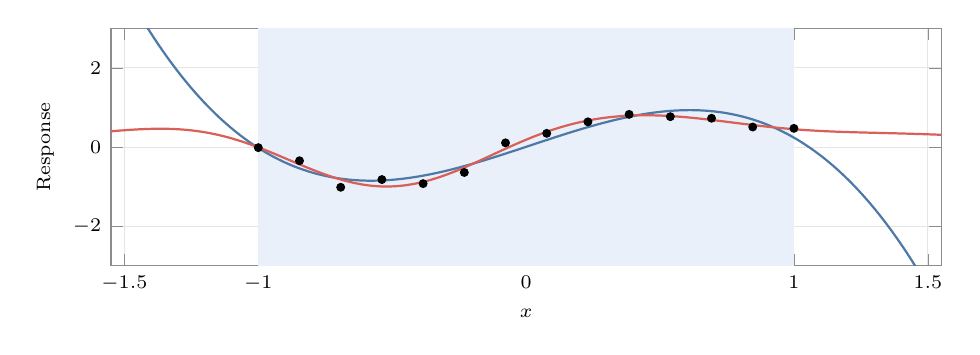
\begin{tikzpicture}
\begin{axis}[width=\linewidth,height=4.6cm,font=\scriptsize,
tick label style={font=\scriptsize},label style={font=\scriptsize},
axis line style={black!45},tick style={black!45},grid=major,grid style={black!10},
scaled ticks=false,xlabel={$x$},ylabel={Response},xmin=-1.05,xmax=1.05,
ymin=-1.6,ymax=1.6,clip=true,unbounded coords=jump,xmin=-1.55,xmax=1.55,ymin=-3,ymax=3,xtick={-1.5,-1,0,1,1.5}]
\path[fill=definitionblue,draw=none] (axis cs:-1,-3) rectangle (axis cs:1,3);
\addplot[blueplot,thick] coordinates {(-1.55,4.643493) (-1.5370833,4.4732915) (-1.5241667,4.3063759) (-1.51125,4.1427188) (-1.4983333,3.9822929) (-1.4854167,3.8250707) (-1.4725,3.6710251) (-1.4595833,3.5201287) (-1.4466667,3.3723542) (-1.43375,3.2276742) (-1.4208333,3.0860614) (-1.4079167,2.9474885) (-1.395,2.8119282) (-1.3820833,2.6793531) (-1.3691667,2.5497359) (-1.35625,2.4230493) (-1.3433333,2.2992659) (-1.3304167,2.1783585) (-1.3175,2.0602997) (-1.3045833,1.9450621) (-1.2916667,1.8326185) (-1.27875,1.7229416) (-1.2658333,1.6160039) (-1.2529167,1.5117782) (-1.24,1.4102371) (-1.2270833,1.3113534) (-1.2141667,1.2150996) (-1.20125,1.1214486) (-1.1883333,1.0303728) (-1.1754167,0.9418451) (-1.1625,0.85583807) (-1.1495833,0.77232439) (-1.1366667,0.69127676) (-1.12375,0.61266783) (-1.1108333,0.53647029) (-1.0979167,0.46265681) (-1.085,0.39120005) (-1.0720833,0.3220727) (-1.0591667,0.25524743) (-1.04625,0.19069691) (-1.0333333,0.12839382) (-1.0204167,0.068310831) (-1.0075,0.010420613) (-0.99458333,-0.045304157) (-0.98166667,-0.098890806) (-0.96875,-0.15036666) (-0.95583333,-0.19975904) (-0.94291667,-0.24709529) (-0.93,-0.29240271) (-0.91708333,-0.33570865) (-0.90416667,-0.37704042) (-0.89125,-0.41642535) (-0.87833333,-0.45389078) (-0.86541667,-0.48946401) (-0.8525,-0.52317239) (-0.83958333,-0.55504323) (-0.82666667,-0.58510387) (-0.81375,-0.61338163) (-0.80083333,-0.63990383) (-0.78791667,-0.66469781) (-0.775,-0.68779088) (-0.76208333,-0.70921038) (-0.74916667,-0.72898363) (-0.73625,-0.74713795) (-0.72333333,-0.76370068) (-0.71041667,-0.77869914) (-0.6975,-0.79216065) (-0.68458333,-0.80411255) (-0.67166667,-0.81458215) (-0.65875,-0.82359679) (-0.64583333,-0.83118378) (-0.63291667,-0.83737047) (-0.62,-0.84218416) (-0.60708333,-0.8456522) (-0.59416667,-0.8478019) (-0.58125,-0.84866059) (-0.56833333,-0.8482556) (-0.55541667,-0.84661426) (-0.5425,-0.84376388) (-0.52958333,-0.8397318) (-0.51666667,-0.83454534) (-0.50375,-0.82823184) (-0.49083333,-0.8208186) (-0.47791667,-0.81233297) (-0.465,-0.80280227) (-0.45208333,-0.79225382) (-0.43916667,-0.78071495) (-0.42625,-0.76821298) (-0.41333333,-0.75477525) (-0.40041667,-0.74042907) (-0.3875,-0.72520179) (-0.37458333,-0.70912071) (-0.36166667,-0.69221317) (-0.34875,-0.67450649) (-0.33583333,-0.656028) (-0.32291667,-0.63680503) (-0.31,-0.6168649) (-0.29708333,-0.59623494) (-0.28416667,-0.57494247) (-0.27125,-0.55301483) (-0.25833333,-0.53047933) (-0.24541667,-0.5073633) (-0.2325,-0.48369407) (-0.21958333,-0.45949897) (-0.20666667,-0.43480532) (-0.19375,-0.40964045) (-0.18083333,-0.38403169) (-0.16791667,-0.35800635) (-0.155,-0.33159177) (-0.14208333,-0.30481527) (-0.12916667,-0.27770419) (-0.11625,-0.25028584) (-0.10333333,-0.22258754) (-0.090416667,-0.19463664) (-0.0775,-0.16646045) (-0.064583333,-0.13808631) (-0.051666667,-0.10954152) (-0.03875,-0.080853435) (-0.025833333,-0.052049365) (-0.012916667,-0.023156641) (0,0.0057974129) (0.012916667,0.034785469) (0.025833333,0.063780201) (0.03875,0.092754283) (0.051666667,0.12168039) (0.064583333,0.15053119) (0.0775,0.17927937) (0.090416667,0.20789759) (0.10333333,0.23635852) (0.11625,0.26463486) (0.12916667,0.29269925) (0.14208333,0.32052439) (0.155,0.34808294) (0.16791667,0.37534758) (0.18083333,0.40229098) (0.19375,0.42888582) (0.20666667,0.45510477) (0.21958333,0.48092049) (0.2325,0.50630568) (0.24541667,0.53123299) (0.25833333,0.55567511) (0.27125,0.57960471) (0.28416667,0.60299446) (0.29708333,0.62581704) (0.31,0.64804511) (0.32291667,0.66965136) (0.33583333,0.69060845) (0.34875,0.71088907) (0.36166667,0.73046588) (0.37458333,0.74931156) (0.3875,0.76739878) (0.40041667,0.78470021) (0.41333333,0.80118854) (0.42625,0.81683643) (0.43916667,0.83161655) (0.45208333,0.84550159) (0.465,0.85846421) (0.47791667,0.87047709) (0.49083333,0.8815129) (0.50375,0.89154432) (0.51666667,0.90054402) (0.52958333,0.90848467) (0.5425,0.91533895) (0.55541667,0.92107953) (0.56833333,0.92567909) (0.58125,0.92911029) (0.59416667,0.93134582) (0.60708333,0.93235834) (0.62,0.93212053) (0.63291667,0.93060507) (0.64583333,0.92778462) (0.65875,0.92363187) (0.67166667,0.91811948) (0.68458333,0.91122013) (0.6975,0.90290649) (0.71041667,0.89315124) (0.72333333,0.88192705) (0.73625,0.86920659) (0.74916667,0.85496254) (0.76208333,0.83916758) (0.775,0.82179437) (0.78791667,0.80281558) (0.80083333,0.7822039) (0.81375,0.759932) (0.82666667,0.73597255) (0.83958333,0.71029822) (0.8525,0.68288169) (0.86541667,0.65369564) (0.87833333,0.62271272) (0.89125,0.58990563) (0.90416667,0.55524703) (0.91708333,0.5187096) (0.93,0.48026601) (0.94291667,0.43988893) (0.95583333,0.39755104) (0.96875,0.35322502) (0.98166667,0.30688352) (0.99458333,0.25849924) (1.0075,0.20804485) (1.0204167,0.15549301) (1.0333333,0.1008164) (1.04625,0.043987692) (1.0591667,-0.015020433) (1.0720833,-0.076235307) (1.085,-0.13968425) (1.0979167,-0.2053946) (1.1108333,-0.27339367) (1.12375,-0.3437088) (1.1366667,-0.41636731) (1.1495833,-0.49139652) (1.1625,-0.56882376) (1.1754167,-0.64867635) (1.1883333,-0.73098164) (1.20125,-0.81576693) (1.2141667,-0.90305956) (1.2270833,-0.99288685) (1.24,-1.0852761) (1.2529167,-1.1802547) (1.2658333,-1.27785) (1.27875,-1.3780892) (1.2916667,-1.4809996) (1.3045833,-1.5866088) (1.3175,-1.6949438) (1.3304167,-1.8060322) (1.3433333,-1.9199011) (1.35625,-2.0365779) (1.3691667,-2.15609) (1.3820833,-2.2784647) (1.395,-2.4037293) (1.4079167,-2.5319111) (1.4208333,-2.6630375) (1.43375,-2.7971358) (1.4466667,-2.9342332) (1.4595833,-3.0743572) (1.4725,-3.2175351) (1.4854167,-3.3637941) (1.4983333,-3.5131617) (1.51125,-3.6656651) (1.5241667,-3.8213316) (1.5370833,-3.9801887) (1.55,-4.1422635)};
\addplot[redplot,thick] coordinates {(-1.55,0.39811445) (-1.5370833,0.40533569) (-1.5241667,0.41234716) (-1.51125,0.41910478) (-1.4983333,0.42556266) (-1.4854167,0.43167323) (-1.4725,0.43738745) (-1.4595833,0.44265496) (-1.4466667,0.44742429) (-1.43375,0.45164306) (-1.4208333,0.45525826) (-1.4079167,0.45821648) (-1.395,0.46046417) (-1.3820833,0.46194793) (-1.3691667,0.46261484) (-1.35625,0.46241271) (-1.3433333,0.46129043) (-1.3304167,0.45919832) (-1.3175,0.45608839) (-1.3045833,0.45191474) (-1.2916667,0.44663386) (-1.27875,0.44020495) (-1.2658333,0.43259028) (-1.2529167,0.42375549) (-1.24,0.4136699) (-1.2270833,0.4023068) (-1.2141667,0.38964377) (-1.20125,0.37566289) (-1.1883333,0.36035105) (-1.1754167,0.34370012) (-1.1625,0.32570721) (-1.1495833,0.3063748) (-1.1366667,0.2857109) (-1.12375,0.2637292) (-1.1108333,0.24044915) (-1.0979167,0.21589599) (-1.085,0.19010083) (-1.0720833,0.16310062) (-1.0591667,0.1349381) (-1.04625,0.10566177) (-1.0333333,0.075325754) (-1.0204167,0.043989697) (-1.0075,0.011718572) (-0.99458333,-0.021417503) (-0.98166667,-0.055343486) (-0.96875,-0.089979674) (-0.95583333,-0.12524198) (-0.94291667,-0.16104222) (-0.93,-0.19728849) (-0.91708333,-0.23388545) (-0.90416667,-0.27073475) (-0.89125,-0.30773538) (-0.87833333,-0.34478406) (-0.86541667,-0.38177571) (-0.8525,-0.4186038) (-0.83958333,-0.45516081) (-0.82666667,-0.49133868) (-0.81375,-0.5270292) (-0.80083333,-0.56212448) (-0.78791667,-0.5965174) (-0.775,-0.63010198) (-0.76208333,-0.66277385) (-0.74916667,-0.69443067) (-0.73625,-0.7249725) (-0.72333333,-0.75430223) (-0.71041667,-0.78232594) (-0.6975,-0.80895329) (-0.68458333,-0.83409783) (-0.67166667,-0.8576774) (-0.65875,-0.87961438) (-0.64583333,-0.89983603) (-0.63291667,-0.91827476) (-0.62,-0.9348684) (-0.60708333,-0.94956039) (-0.59416667,-0.96230006) (-0.58125,-0.97304276) (-0.56833333,-0.98175006) (-0.55541667,-0.98838992) (-0.5425,-0.99293675) (-0.52958333,-0.99537153) (-0.51666667,-0.99568191) (-0.50375,-0.9938622) (-0.49083333,-0.98991344) (-0.47791667,-0.98384336) (-0.465,-0.97566634) (-0.45208333,-0.96540336) (-0.43916667,-0.95308194) (-0.42625,-0.93873597) (-0.41333333,-0.92240561) (-0.40041667,-0.90413709) (-0.3875,-0.88398256) (-0.37458333,-0.86199982) (-0.36166667,-0.83825211) (-0.34875,-0.81280782) (-0.33583333,-0.78574021) (-0.32291667,-0.7571271) (-0.31,-0.72705052) (-0.29708333,-0.69559634) (-0.28416667,-0.66285395) (-0.27125,-0.62891582) (-0.25833333,-0.5938771) (-0.24541667,-0.55783523) (-0.2325,-0.52088951) (-0.21958333,-0.48314066) (-0.20666667,-0.44469037) (-0.19375,-0.4056409) (-0.18083333,-0.36609459) (-0.16791667,-0.3261535) (-0.155,-0.28591892) (-0.14208333,-0.24549098) (-0.12916667,-0.20496826) (-0.11625,-0.16444736) (-0.10333333,-0.12402261) (-0.090416667,-0.083785624) (-0.0775,-0.043825056) (-0.064583333,-0.0042262585) (-0.051666667,0.034928981) (-0.03875,0.073562679) (-0.025833333,0.11160087) (-0.012916667,0.14897381) (0,0.18561607) (0.012916667,0.22146674) (0.025833333,0.25646942) (0.03875,0.29057234) (0.051666667,0.32372836) (0.064583333,0.35589496) (0.0775,0.38703419) (0.090416667,0.41711261) (0.10333333,0.44610122) (0.11625,0.47397531) (0.12916667,0.50071431) (0.14208333,0.52630167) (0.155,0.55072468) (0.16791667,0.57397424) (0.18083333,0.5960447) (0.19375,0.61693364) (0.20666667,0.63664164) (0.21958333,0.65517207) (0.2325,0.6725309) (0.24541667,0.68872645) (0.25833333,0.70376919) (0.27125,0.71767154) (0.28416667,0.73044771) (0.29708333,0.74211345) (0.31,0.75268596) (0.32291667,0.76218367) (0.33583333,0.77062615) (0.34875,0.77803396) (0.36166667,0.78442854) (0.37458333,0.78983217) (0.3875,0.79426781) (0.40041667,0.79775912) (0.41333333,0.80033036) (0.42625,0.80200639) (0.43916667,0.80281265) (0.45208333,0.80277512) (0.465,0.80192037) (0.47791667,0.80027552) (0.49083333,0.79786827) (0.50375,0.79472694) (0.51666667,0.79088046) (0.52958333,0.78635839) (0.5425,0.78119095) (0.55541667,0.77540901) (0.56833333,0.76904413) (0.58125,0.76212852) (0.59416667,0.75469506) (0.60708333,0.74677727) (0.62,0.73840926) (0.63291667,0.72962573) (0.64583333,0.72046188) (0.65875,0.71095335) (0.67166667,0.70113616) (0.68458333,0.6910466) (0.6975,0.68072112) (0.71041667,0.67019625) (0.72333333,0.65950845) (0.73625,0.64869397) (0.74916667,0.63778873) (0.76208333,0.62682817) (0.775,0.61584708) (0.78791667,0.60487947) (0.80083333,0.59395839) (0.81375,0.58311579) (0.82666667,0.57238238) (0.83958333,0.56178744) (0.8525,0.55135872) (0.86541667,0.54112227) (0.87833333,0.53110235) (0.89125,0.5213213) (0.90416667,0.51179942) (0.91708333,0.5025549) (0.93,0.49360377) (0.94291667,0.48495979) (0.95583333,0.47663445) (0.96875,0.46863695) (0.98166667,0.46097416) (0.99458333,0.45365067) (1.0075,0.44666878) (1.0204167,0.44002857) (1.0333333,0.43372799) (1.04625,0.42776287) (1.0591667,0.42212708) (1.0720833,0.4168126) (1.085,0.41180965) (1.0979167,0.40710682) (1.1108333,0.40269124) (1.12375,0.39854869) (1.1366667,0.39466376) (1.1495833,0.39102006) (1.1625,0.38760034) (1.1754167,0.38438667) (1.1883333,0.38136062) (1.20125,0.37850343) (1.2141667,0.37579616) (1.2270833,0.37321986) (1.24,0.37075572) (1.2529167,0.36838524) (1.2658333,0.36609034) (1.27875,0.36385351) (1.2916667,0.36165794) (1.3045833,0.35948761) (1.3175,0.35732739) (1.3304167,0.35516313) (1.3433333,0.35298178) (1.35625,0.35077135) (1.3691667,0.34852108) (1.3820833,0.34622137) (1.395,0.34386389) (1.4079167,0.34144152) (1.4208333,0.33894842) (1.43375,0.33637995) (1.4466667,0.33373271) (1.4595833,0.33100447) (1.4725,0.32819414) (1.4854167,0.32530174) (1.4983333,0.32232832) (1.51125,0.31927589) (1.5241667,0.31614741) (1.5370833,0.31294664) (1.55,0.30967811)};
\addplot[only marks,mark=*,mark size=1.4pt,black] coordinates {(-1,-0.014539702) (-0.84615385,-0.34516883) (-0.69230769,-1.0151104) (-0.53846154,-0.82009194) (-0.38461538,-0.92297015) (-0.23076923,-0.64102463) (-0.076923077,0.10647764) (0.076923077,0.3460617) (0.23076923,0.63699851) (0.38461538,0.82531436) (0.53846154,0.76750888) (0.69230769,0.72707693) (0.84615385,0.50661061) (1,0.47271884)};
\end{axis}
\end{tikzpicture}
\end{column}
\begin{column}{.40\textwidth}\small
\textcolor{blueplot}{\textbf{Cubic OLS}}\par\medskip
Powers continue globally.\par\bigskip
\textcolor{redplot}{\textbf{RBF kernel ridge}}\par\medskip
Local similarities fade.\par\bigskip
\large Neither curve supplies evidence about an unseen regime.
\end{column}
\end{columns}
\vfill
\begin{takeaway}Match validation to the prediction domain. Feature expansion preserves the need for judgment.\end{takeaway}
\note{Suggested time: 3 minutes. The blue band is the training input range [-1,1]. The two curves show a degree-three OLS fit and RBF KRR with ell=.4 and lambda=.001, each fit only to the same observations in that window. Both curves extend outside it by mathematical convention. The polynomial grows according to its highest-degree terms. For the RBF with an unpenalized intercept, as a new input moves infinitely far from every training input, raw kernel values tend to zero and the prediction tends to the fitted intercept b, which is not necessarily the sample response mean. With the centered formula and sum(alpha)=0, this limit is y_bar-(K1/n) transpose alpha. Do not say that centered RBF predictions always revert to y_bar. The plotted finite window need not have reached that limit. Ask students how they would validate for a factory switching to a much larger production range: an ordinary random split within the old range cannot directly test that new regime. The model and the dataset jointly determine what can be assessed. End with the lab: compare degree, basis, penalty, and bandwidth while keeping the validation split fixed.}
\end{frame}

% Slide 73 | synthesis
\begin{frame}{Return to tomorrow's electricity forecast}
\lead{Choose the model, solver, penalty, and representation for the prediction task}
\begin{center}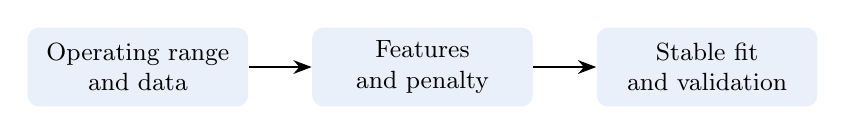
\begin{tikzpicture}[font=\small,every node/.style={align=center}]
\node[fill=definitionblue,rounded corners,minimum width=2.8cm,minimum height=1.0cm] (a) {Operating range\\and data};
\node[fill=definitionblue,rounded corners,minimum width=2.8cm,minimum height=1.0cm,right=.8cm of a] (b) {Features\\and penalty};
\node[fill=definitionblue,rounded corners,minimum width=2.8cm,minimum height=1.0cm,right=.8cm of b] (c) {Stable fit\\and validation};
\draw[-{Stealth},thick] (a)--(b);\draw[-{Stealth},thick] (b)--(c);
\end{tikzpicture}\end{center}
\small\begin{itemize}\setlength{\itemsep}{8pt}
\item Can you derive the LSQ solution and state its rank condition?
\item Can you distinguish numerical error, sensitivity, and overfitting?
\item What evidence justifies Ridge, Lasso, polynomial features, or a kernel?
\end{itemize}\vfill
\begin{takeaway}Begin with an interpretable benchmark; add complexity when validation supports it.\end{takeaway}
\note{Suggested time: 5 minutes. Return to the production plan used at the beginning and ask students to outline a complete forecasting procedure. They should specify which inputs are available before the target is observed, how the chronological split matches future deployment, and what baseline will be used. Ask a volunteer to derive the normal equations and another to explain why an invertible Gram matrix can still be a poor computational route. Then ask when shrinkage or a richer representation could improve generalization. A low training error does not answer those questions. Reserve two minutes for individual written answers and three minutes for discussion. The five sections should now form one chain: motivation, formulation, stability, regularization, and representation.}
\end{frame}



\begin{frame}[t]{Statistical assumptions}
	\begin{definitionbox}
		\[
		\begin{gathered}
			y=X \theta^*+\varepsilon,\qquad X\in\R^{n\times p},\qquad \rank(X)=p,\\[5pt]
			\E[\varepsilon\mid X]=0,\qquad
			\Cov(\varepsilon\mid X)=\sigma^2 I_n.
		\end{gathered}
		\]
	\end{definitionbox}
	\small
	\begin{itemize}\setlength{\itemsep}{.18cm}
		\item The conditional mean is linear in the chosen features.
		\item $p$ counts every fitted coefficient, including an intercept.
		\item For now, condition on $X$ and average over training noise.
		\item Gaussian noise is unnecessary for the expectation identities.
	\end{itemize}
	\vfill
	\begin{takeaway}Full column rank gives $n\ge p$. Equal noise variance and zero conditional mean are substantive assumptions.\end{takeaway}
	\note{State these assumptions before writing an inverse. The noise coordinates need not be independent for the next mean and covariance calculations: zero conditional cross-covariances and a common variance suffice. Full rank permits n=p, although an unbiased residual variance estimator later requires n>p. A deterministic intercept column is included in p. The special random Gaussian design result later has a different, explicit no-intercept assumption. The parameter theta-star is fixed across repeated noise draws. General references: Hastie, Tibshirani and Friedman, The Elements of Statistical Learning, Chapters 3 and 7.}
\end{frame}



\begin{frame}[t]{Which error are we averaging?}
	\small\renewcommand{\arraystretch}{1.65}
	\begin{tabularx}{\textwidth}{@{}lY@{}}
		\toprule
		\textbf{Quantity}&\textbf{Squared error for one fitted model}\\
		\midrule
		Training error&$\widehat R_{\rm train}=\frac1n\lVert y-X\olshat\rVert^2$\\
		Parameter error&$\lVert\olserr\rVert^2$\\
		Mean prediction error at $X$&$\mathcal E_X=\frac1n\lVert X\olshat-X\olsstar\rVert^2$\\
		Fresh-response error at $X$&$\frac1n\lVert y'-X\olshat\rVert^2$, with independent new noise\\
		\bottomrule
	\end{tabularx}
	\vfill
	\begin{takeaway}Predicting the true mean and predicting a noisy response differ by irreducible noise.\end{takeaway}
	\note{Read each target aloud. Training error compares the fit with the responses that produced the fit. Mean prediction error compares the fit with the unobserved true means. Fresh-response error uses y-prime=X theta-star+epsilon-prime at the same rows, with a new zero-mean noise vector independent of the training noise conditional on X and covariance sigma-squared I. Parameter error depends on feature units. Every displayed squared error uses the full square, without a factor of one half: the previous optimization objective J is training MSE divided by two. New random input locations appear later.}
\end{frame}




\begin{frame}[t]{OLS estimation error}
	\lead{Substitute the data-generating model into the closed-form solution}
	\begin{definitionbox}
		\[
		\begin{aligned}
			\olshat&=(X^{\mathsf T}X)^{-1}X^{\mathsf T}y\\[5pt]
			&=(X^{\mathsf T}X)^{-1}X^{\mathsf T}(X\olsstar+\varepsilon)\\[5pt]
			&=\olsstar+(X^{\mathsf T}X)^{-1}X^{\mathsf T}\varepsilon.
		\end{aligned}
		\]
	\end{definitionbox}
	\uncover<2->{\[
		\boxed{\olserr=A\varepsilon},\qquad
		A=(X^{\mathsf T}X)^{-1}X^{\mathsf T}\in\R^{p\times n}.
		\]}
		
		The OLS estimator is unbiased: $\mathbb{E}[\hat{\theta}] = \theta^*$.
\end{frame}

% 05
\begin{frame}[t]{Unbiasedness and covariance}
	\begin{definitionbox}
		\[
		\begin{aligned}
			\E[\olshat\mid X]
			&=\olsstar+A\E[\varepsilon\mid X]=\olsstar,\\[7pt]
			\Cov(\olshat\mid X)
			&=A\Cov(\varepsilon\mid X)A^{\mathsf T}\\[4pt]
			&=\sigma^2(X^{\mathsf T}X)^{-1}X^{\mathsf T}X(X^{\mathsf T}X)^{-1}\\[4pt]
			&=\boxed{\sigma^2(X^{\mathsf T}X)^{-1}}.
		\end{aligned}
		\]
	\end{definitionbox}
	\vfill
	\begin{takeaway}OLS is centered at the true parameter. Its variance can still be large.\end{takeaway}
	\note{Unbiasedness concerns an average over hypothetical repeated datasets with the same inputs. It does not imply that a particular fit is accurate. Check the p by p covariance dimensions. The sandwich formula A Omega A-transpose remains valid under a general conditional noise covariance Omega; replacing it with sigma-squared times the inverse Gram matrix then requires the stated homoskedastic, uncorrelated-noise assumption.}
\end{frame}

% 06
\begin{frame}[t]{Expected squared parameter error}
	\lead{For any random vector $z$, $\E\lVert z\rVert^2=\lVert\E z\rVert^2+\olstr(\Cov(z))$}
	\begin{definitionbox}
		\[
		\begin{aligned}
			\E[\lVert\olserr\rVert^2\mid X]
			&=\underbrace{\lVert\E[\olshat\mid X]-\olsstar\rVert^2}_{0}
			+\olstr\!\left(\Cov(\olshat\mid X)\right)\\[7pt]
			&=\sigma^2\olstr\!\left((X^{\mathsf T}X)^{-1}\right)\\[7pt]
			&=\boxed{\sigma^2\sum_{j=1}^{p}\frac1{s_j^2}},\qquad s_j>0.
		\end{aligned}
		\]
	\end{definitionbox}
	\small Here $s_j$ are the singular values of $X$.
	\note{For the trace identity, write the squared norm as trace of zz-transpose and use linearity of expectation, then decompose the second moment into covariance plus the outer product of the mean. In the last line, X-transpose X has eigenvalues s-j squared. This is coefficient error in the chosen coordinate system; rescaling features changes its numerical value. The condition number alone does not determine the error, because the absolute singular-value scale also matters.}
\end{frame}

% 07
\begin{frame}[t]{Ill-conditioning and statistical error}
	\begin{columns}[T,onlytextwidth]
		\begin{column}{.59\textwidth}\olsfig{spectrum}\end{column}
		\begin{column}{.38\textwidth}\small
			For $X=USV^{\mathsf T}$,
			\[
			\Var(v_j^{\mathsf T}\olshat\mid X)=\frac{\sigma^2}{s_j^2}.
			\]
			\vspace{.15cm}
			\olsprompt{Which direction dominates?}
			\uncover<2->{\par\vspace{.2cm}
				With $\sigma^2=1$,
				\[\E\lVert\olserr\rVert^2
				\approx 101.12.\]
				The weakest direction contributes $100$.}
		\end{column}
	\end{columns}
	\vfill
	\begin{takeaway}QR and SVD improve numerical computation. Weakly observed directions still have statistical uncertainty.\end{takeaway}
	\note{All expectations here condition on the displayed design spectrum. The four variance contributions are 0.01, 1/9, 1, and 100, totaling 101.121111. Ask for the dominant direction before revealing the total. This connects the earlier ill-conditioning lecture to sampling uncertainty in exact arithmetic. Ridge can reduce variance along these directions by accepting bias, while additional informative observations can increase the weak singular values. Rescaling can improve numerical units without creating information.}
\end{frame}

% 08
\begin{frame}[t]{Prediction error at one input}
	\lead{Let $x_0\in\R^p$ be a fixed feature vector, including an intercept if used}
	\begin{definitionbox}
		\[
		\begin{aligned}
			\E[(x_0^{\mathsf T}\olshat-x_0^{\mathsf T}\olsstar)^2\mid X]
			&=x_0^{\mathsf T}\Cov(\olshat\mid X)x_0\\[6pt]
			&=\boxed{\sigma^2x_0^{\mathsf T}(X^{\mathsf T}X)^{-1}x_0}.
		\end{aligned}
		\]
	\end{definitionbox}
	\uncover<2->{\small For a fresh response $y_0=x_0^{\mathsf T}\olsstar+\varepsilon_0$,
		\[
		\E[(y_0-x_0^{\mathsf T}\olshat)^2\mid X]
		=\underbrace{\sigma^2}_{\text{new response noise}}
		+\underbrace{\sigma^2x_0^{\mathsf T}(X^{\mathsf T}X)^{-1}x_0}_{\text{estimation error}}.
		\]}
	\note{The first display averages over the training noise only. In the second, also average over epsilon-zero, which is independent of the training noise, has mean zero, and variance sigma-squared. The cross term vanishes. For a fixed x-zero, the quadratic form is a leverage-like measure of how well that feature direction is supported by the observed design. Large coefficient variance need not imply equally large prediction variance at every input.}
\end{frame}
% 10





% 15
\begin{frame}[t]{Prediction at new random inputs}
	\lead{The test pair $(x_0,\varepsilon_0)$ is independent of the training sample. Let $Q=\E[x_0x_0^{\mathsf T}]$}
	\begin{definitionbox}
		\[
		\begin{aligned}
			R(\theta)&=\E_{x_0,\varepsilon_0}[(y_0-x_0^{\mathsf T}\theta)^2],\\[5pt]
			y_0&=x_0^{\mathsf T}\olsstar+\varepsilon_0,
			\quad \E[\varepsilon_0\mid x_0]=0,
			\quad \E[\varepsilon_0^2\mid x_0]=\sigma^2,\\[5pt]
			R(\theta)-R(\olsstar)
			&=(\theta-\olsstar)^{\mathsf T}Q(\theta-\olsstar),
			\quad R(\olsstar)=\sigma^2.
		\end{aligned}
		\]
	\end{definitionbox}
	\small For a realized $\olshat$, $R(\olshat)$ averages over a new test example.
	\vfill
	\begin{takeaway}$Q$ is a second-moment matrix. It equals a covariance matrix only when the feature mean is zero.\end{takeaway}
	\note{First define R at a deterministic theta. After training, substitute the realized theta-hat: the remaining expectation in the definition still averages only over the test example. The next slide also averages over training noise. A constant intercept coordinate makes the feature vector nonzero-mean, so calling Q a covariance matrix would be incorrect. Finite second moments are required. The test model must share the same theta-star for this expression; a change in the true relationship adds further terms.}
\end{frame}

% 16
\begin{frame}[t]{Expected excess prediction risk}
	\lead{Average the population risk over the noise that produced $\olshat$}
	\begin{definitionbox}
		\[
		\begin{aligned}
			\E[R(\olshat)-R(\olsstar)\mid X]
			&=\E[(\olserr)^{\mathsf T}Q(\olserr)\mid X]\\[5pt]
			&=\olstr\!\left(Q\Cov(\olshat\mid X)\right)\\[5pt]
			&=\boxed{\sigma^2\olstr\!\left(Q(X^{\mathsf T}X)^{-1}\right)}.
		\end{aligned}
		\]
	\end{definitionbox}
	\uncover<2->{\small If test inputs are uniform over the rows of $X$, their conditional second moment is $X^{\mathsf T}X/n$, recovering $\sigma^2p/n$.}
	\vfill
	\begin{takeaway}Error depends on how the test-input directions align with the directions learned from the training design.\end{takeaway}
	\note{Use trace(Q zz-transpose) for the quadratic form and the zero conditional mean of the estimation error. The initial result assumes an independent test-input distribution with fixed second moment Q. The empirical-input example on the reveal is a separate conditional evaluation rule: sample a row index uniformly given X, so Q becomes Q-X=X-transpose X/n. Add sigma-squared to the displayed excess risk to obtain total response prediction risk. This is an exact conditional identity under the assumptions, not yet a distribution-free generalization guarantee.}
\end{frame}

% 17
\begin{frame}[t]{An expected generalization bound}
	\lead{A lower bound on the design eigenvalues gives a usable upper bound on risk}
	\begin{definitionbox}
		\[
		\begin{gathered}
			\widehat G=\frac1nX^{\mathsf T}X,\qquad
			\lambda_{\min}(\widehat G)\ge a>0,\\[6pt]
			\E[R(\olshat)-R(\olsstar)\mid X]
			=\frac{\sigma^2}{n}\olstr(Q\widehat G^{-1})
			\le \boxed{\frac{\sigma^2\olstr(Q)}{na}}.
		\end{gathered}
		\]
	\end{definitionbox}
	\small If $Q=I_p$, the bound becomes $\sigma^2p/(na)$.\par
	\vspace{.15cm}
	\uncover<2->{\olsprompt{When does an $O(p/n)$ statement become informative?}\par
		\small When the design remains well supported: $a$ stays away from zero.}
	\note{Since G-hat is at least a times the identity in positive-semidefinite order, its inverse is at most the identity divided by a. Multiplying within a trace by positive-semidefinite Q preserves the scalar inequality. This is a conditional bound in expectation over training noise. If X is random, a claim that its minimum eigenvalue exceeds a with high probability needs a separate design-distribution assumption and concentration argument. Do not silently replace this condition with n greater than p. In isotropic feature units Q=I, the bound shows the p/n scale and its dependence on a.}
\end{frame}



% 19
\begin{frame}[t]{Learning curve under Gaussian inputs}
	\begin{columns}[T,onlytextwidth]
		\begin{column}{.59\textwidth}\olsfig{random-design}\end{column}
		\begin{column}{.38\textwidth}\small
			$p=10$, Gaussian inputs, no intercept.\par\medskip
			\renewcommand{\arraystretch}{1.4}
			\begin{tabular}{@{}rr@{}}
				\toprule $n$&Excess risk$/\sigma^2$\\\midrule
				$20$&$10/9\approx1.111$\\
				$50$&$10/39\approx0.256$\\
				$100$&$10/89\approx0.112$\\\bottomrule
			\end{tabular}\par
			\vspace{.3cm}
			\olsprompt{How many samples are enough?}\par
			Both $p$ and the tolerated error matter.
		\end{column}
	\end{columns}
\end{frame}


\begin{frame}{Regression Evaluation Metrics}
	\small
	\begin{itemize}
		\setlength{\itemsep}{0.8em}
		
		\item  $
		\mathrm{MAE}=\frac{1}{n}\sum_{i=1}^{n}|y_i-\hat{y}_i|$		
		\item $
		\mathrm{MSE}=\frac{1}{n}\sum_{i=1}^{n}(y_i-\hat{y}_i)^2$
		
		\item 
		$
		\mathrm{RMSE}=\sqrt{\frac{1}{n}\sum_{i=1}^{n}(y_i-\hat{y}_i)^2}
		$
		
		\item
		$
		R^2=1-\frac{\sum_{i=1}^{n}(y_i-\hat{y}_i)^2}
		{\sum_{i=1}^{n}(y_i-\bar{y})^2}
		$
		
		\item 
		$
		R_{\mathrm{adj}}^2=1-(1-R^2)\frac{n-1}{n-p}
		$
		
		\item
		$
		\mathrm{MAPE}=\frac{100\%}{n}\sum_{i=1}^{n}
		\left|\frac{y_i-\hat{y}_i}{y_i}\right|
		$
	\end{itemize}
\end{frame}
% 20
\end{document}
